% !TEX encoding = UTF-8
% !TEX TS-program = pdflatex
% !TEX root = ../nt.tex
% !TEX spellcheck = it-IT

%************************************************
\chapter{MODELLO LOGICO}
\label{cap:logical}
%************************************************\\

\section{SQL QUERY: Le interrogazioni del database}

Per effettuare un'interrogazione del database bisogna avere una procedura sistematica che, dato un problema, ci consente di trovare una soluzione e verificarla in diversi casi di test in modo da appurare che sia una soluzione generale e non particolare.  

\underline{Esempio}: Una lista di clienti è una query sull'entità di tipo di cliente, ma non ci basta una sola query perché avremmo bisogno di vedere i clienti in ordine di nome, di luogo, di residenza, di data di nascita, ecc.   

\begin{center}
\begin{figure}[H]
\centering
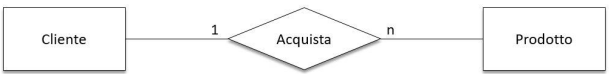
\includegraphics[scale=0.8]{figures/cliente_acquista_prodotto.png}
\caption{Cliente Acquista Prodotto} 
\end{figure}
\end{center}

Le query devono rispondere ottimamente qualunque sia il criterio di filtraggio e devono essere robuste: ad esempio esiste la possibilità di, non conoscendo username e password, ma inserendo righe di codice in modo opportuno, poter entrare in un database (SQL INJECTION). Bisogna quindi fare attenzione nel momento in cui si scrive una query perché qualcuno potrebbe iniettarvi dei pezzi aggiuntivi. La connessione tra le pagine e il database avviene attraverso un certo numero di query: questo codice deve essere robusto, verificato, sviluppato attraverso procedure precise e rigorose basate sul concetto dell'algebra relazionale. 

Le query sono formule matematiche scritte in algebra relazionale. Il modo migliore per scrivere  una query è capire l'algebra che c'è dietro. 

\begin{center}
\begin{figure}[H]
\centering
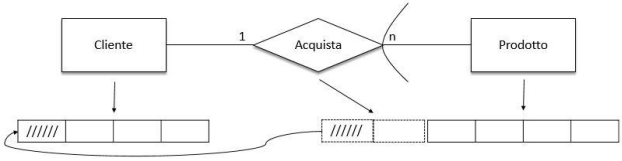
\includegraphics[scale=0.8]{figures/cap_logical.png}
\caption{Cliente Acquista Prodotto - Mapping} 
\end{figure}
\end{center}

Uno schema viene trasformato in tabella in base al tipo di cardinalità della relazione. Queste tabelle d'ora in poi saranno chiamate relazioni. L'algebra relazionale è un'algebra insiemistica in cui  gli insiemi sono rappresentati non da diagrammi di Venn, ma da tabelle, in questo senso si dice  che un database è un insieme di relazioni $(R_i)$ e vincoli o constraints $(C_j)$:

\[
	DB = \{R_i,\ C_j\}
\]

I vincoli sono una serie di regole che utilizzeremo per far sì che i nostri dati restino coerenti,  cioè che il database resti un database. Le caratteristiche principali sono: assenza di ridondanza, minima quantità di NULL, unicità di rappresentazione dell'informazione, ecc.  
L'oggetto di base dell'algebra relazionale, come detto, è la relazione o tabella. Oltre alle relazioni abbiamo un certo numero di operatori: come nell'algebra ci sono i numeri $\{1,2,3,\ \dots\}$ e li combiniamo attraverso operatori $\{+,*,\ \dots\}$, così in quella relazionale esistono operatori unari e binari. Un ulteriore modello è quello dell'algebra booleana dove  esistono operatori unari e binari (ad esempio l'operatore \textit{not} applicato ad un bit 0 fornisce  come risultato 1, mentre \textit{and} applicato a 1 fornisce 0).  


\subsection{ALGEBRA RELAZIONALE}

Tutte le tabelle che vengono fuori dall'algebra relazionale sono calcolate, cioè vengono  create come il risultato di un'espressione, pertanto sono solo viste, non vengono memorizzate  e non occupano spazio. 

\begin{itemize}

\item{\textbf{Operatori Unari}}:

Per quanto riguarda gli operatori unari dell'algebra relazionale: 

\begin{itemize}

\item Il primo tra tutti gli operatori che ci interessano è quello di “\textit{select}”. Si scrive come: 

\[
	\sigma_{<c>}(R)
\]

Questo operatore estrae o seleziona dalla tabella R una nuova tabella fatta dalle stesse colonne della tabella R e dalle sole righe che soddisfano la condizione C (fare riferimento cap. 4 e cap. 8 del libro).

\underline{Esempio} Seleziona $\sigma_{<CLIENT.CITY="LECCE">}(CLIENT)$. Cosa viene fuori da questa espressione? Avremo una nuova tabella chiamata R avente le stesse colonne della tabella clienti e un sottoinsieme delle righe;


\item Il secondo operatore è “project”, così come la select riduce il numero di righe, la project riduce il numero di colonne estraendone solo alcune. Si scrive come:

\[
	\pi_{<col1,\ col2,\ \dots>}(R)
\]

Questo operatore prende un numero selezionato o ridotto delle colonne della tabelle di  partenza;

\item Il terzo operatore è “\textit{rename}”, serve a rinominare determinati attributi. Questo produce una nuova tabella in cui le colonne si chiamano in un altro modo. Si scrive come: 

\[
	\rho_{col1\ as\ new1,\ col2\ as\ new2,\ \dots}(R)
\]

\end{itemize}

\item{\textbf{Operatori Binari}}:

Il secondo gruppo di operatori sono di tipo insiemistico. Questi richiedono che gli oggetti siano  union-compatible, cioè che abbiano le stesse colonne o che si chiamino nella stessa maniera.  Le operazioni che conosciamo sono: 

\begin{itemize}

\item{Unione}: denotata con $R \cup S$. Posso fare quest'operazione solo se la prima e la seconda tabella hanno le stesse colonne, ciò è garantito dalla union-compatible. Lo loro unione è una nuova tabella virtuale in cui ci sono tutte le righe della prima tabella e tutte quelle della seconda;

\item{Intersezione}: denotata con $R \cap S$. Se ho due righe con gli stessi nomi di colonna,  fare l'intersezione degli elementi presenti sia in R che in S significa selezionare gli elementi comuni. La chiave primaria deve garantire che ogni riga sia univocamente definita dato che la teoria dell'algebra relazionale dice che tutti i dati devono essere diversi;

\item{Differenza}: denotata con $R-S = R-(R\cap S)$. È il set di tutti gli elementi che sono inclusi in R ma non in S;

\item{Prodotto cartesiano}: $R \times S$.  Questa operazione genera l'insieme di tutte le possibili coppie $T\{(r_i,s_j)\}$ Immaginiamo che R ed S siano dei concetti o idee, la capacità di creare corrispondenze tra queste genera dei nuovi concetti applicativi. Si intuisce, però, che l'insieme di tutte le coppie possibili è troppo grande (alcune non hanno senso e non servono), perciò eliminiamo le connessioni inutili utilizzando l'operazione di join;

\item{Join}:

\[
	R \Join S := \sigma_{<c>}(R \times C)
\]

Essa è l'operazione chiave dei database. È ciò che facciamo quando scriviamo \textit{SELECT FROM WHERE}. La selezione è la possibilità di estrarre solo alcune colonne da una tabella potendo esprimere la condizione. In altre parole fare la join di due tabelle dal punto di vista dell'algebra relazionale significa attaccare tutti gli elementi corrispondenti. 

\end{itemize}

\underline{Esempio}: Join di due tabelle:

\begin{center}
\begin{figure}[H]
\centering
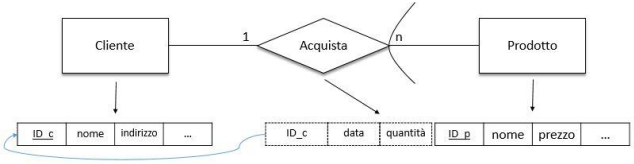
\includegraphics[scale=0.8]{figures/join.png}
\caption{Join di due tabelle} 
\end{figure}
\end{center}

Questa notazione senza righe è ciò che d'ora in poi chiameremo \underline{modello relazionale} (insieme di tabelle più insieme di vincoli), in cui specifichiamo i vincoli di chiave primaria (sottolineata), di chiave esterna $(ID\_c)$ e vincoli di integrità referenziale (freccia).

\end{itemize}

\subsection{Operatore Join}

Analizziamo l'operatore join attraverso uno scenario: supponiamo di avere Mario Rossi  con indirizzo Lecce e Giorgio Bianchi con indirizzo Milano, nel nostro autosalone abbiamo  la macchina 1 che è una Fiat Tipo che ha il prezzo di € 10mila. Inizialmente nel DB non c'è scritto nulla ma nel momento in cui viene venduta ci aggiungiamo le informazioni riguardanti Mario Rossi con la data di acquisto. Fare il prodotto cartesiano delle due tabelle significa avere tutte  le combinazioni o coppie possibili. Se adesso ci facciamo sopra una selezione sulla condizione di join, cioè vogliamo selezionare solo le righe $Prodotto.ID_c = Cliente.ID_c$ vedremo solo le coppie che soddisfano la corrispondenza.   

\begin{center}
\begin{figure}[H]
\centering
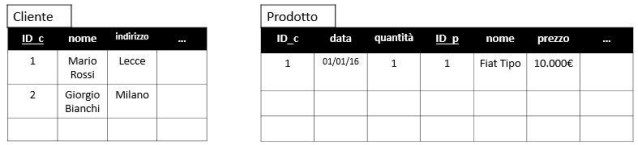
\includegraphics[scale=0.8]{figures/cliente_prodotto_logical.png}
\caption{Scenario logico Cliente/Prodotto} 
\end{figure}
\end{center}

La join è una nuova tabella, che per il momento indichiamo come Cliente-Prodotto, contenente tutte le colonne del cliente $\{c_1, c_2, c_3,\ \dots\}$ e tutte le colonne del prodotto $\{p_1, p_2, p_3,\ \dots\}$ che soddisfano  la condizione di join, ovvero che la chiave esterna di una tabella deve essere uguale alla corrispondente chiave primaria dell'altra tabella (se non ho venduto nessuna macchina la tabella di join sarà vuota).  

\begin{center}
\begin{figure}[H]
\centering
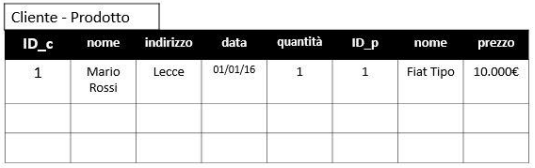
\includegraphics[scale=0.8]{figures/cliente_join_prodotto.png}
\caption{Cliente JOIN Prodotto} 
\end{figure}
\end{center}

In algebra relazionale l'operazione di join è scritta in questo modo: 

\[
	Cliente \Join_{<Prodotto.ID=Cliente.ID_c>}(Prodotto)
\]

Unire le tabelle significa prendere le coppie degli elementi corrispondenti. Come si scrive questa cosa all'interno di una select? Possiamo ad esempio scrivere: 

\begin{lstlisting}[language=SQL]
SELECT  Cliente.nome, Prodotto.nome 
FROM  Cliente JOIN Prodotto ON Prodotto.ID_c = Cliente.ID_c 
WHERE 1 -- (significa prendili tutti)
-- WHERE Prodotto.nome = "Fiat Tipo"
\end{lstlisting}

ove l'ultima \textit{WHERE} commentata è un'ulteriore condizione per cercare tutti i clienti che hanno comperato una Fiat Tipo.

Vediamo ora la join dal punto di vista insiemistico:

\begin{center}
\begin{figure}[H]
\centering
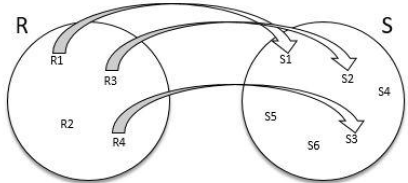
\includegraphics[scale=1]{figures/join_set.png}
\caption{Diagramma Eulero-Venn per una JOIN} 
\end{figure}
\end{center}


\subsubsection{Tipi di Join}

Grazie a questi concetti di base dell'algebra relazionale (più altri che aggiungeremo nelle lezioni successive) possiamo effettuare qualunque tipo di query. Tramite l'algebra relazionale se l'informazione è nel database possiamo estrarla grazie a questi operatori. Potremo aggiungere, inoltre, alcune varianti dell'operazione di join che non sono strettamente necessarie ma sono utili: 

\begin{itemize}

\item{Natural join $\{*\}$}: è l'operazione che si fa quando all'interno di una condizione si specifica esattamente cosa è scritto nel vincolo di integrità referenziale, cioè è la join tra due tabelle quando esiste solo una colonna con lo stesso nome;

\item{Theta join $\{\theta\}$}: è l'operazione che generalizza il concetto di operatore relazionale, cioè quelli che mettono in relazione due termini $\{<,\leq,==,\geq,>\}$. Quest'operazione non si limita alla join (o equi-join) che verifica solo l'uguaglianza tra gli elementi, ma usa un operatore relazionale diverso per ottenere criteri di ordinamento più ampi (mette in confronto due tabelle per vedere tutti gli elementi a seconda della particolare relazione considerata);

\end{itemize}

Ulteriori varianti interessanti dell'operatore join, dal punto di vista insiemistico, sono:

\begin{itemize}

\item{Left outer join $\{=\Join\}$}: è l'operazione che prende tutti gli elementi dell'insieme R e solo i corrispondenti dell'insieme S;
\item{Right outer join $\{\Join=\}$}: è l'operazione che prende tutti gli elementi dell'insieme S e solo i corrispondenti dell'insieme R;
\item{Full outer join $\{=\Join=\}$}:  è l'operazione che prende tutti gli elementi di entrambi gli insiemi, se ci sono delle corrispondenze le mette sulla stessa riga, altrimenti troveremo un NULL (a destra o a sinistra, mai da entrambe le parti).

\end{itemize}

\underline{Ricapitolazione}:

\begin{itemize}

\item Select considera solo alcune righe;
\item Project considera solo alcune colonne;
\item Unione, intersezione e differenza sono i medesimi concetti elementari di teoria degli insiemi;
\item Join mette in relazioni oggetti che stanno in tabelle diverse, crea una nuova tabella con tutte le colonne di entrambe le tabelle inziali ma solo le righe dove è presente una corrispondenza. Questa è l'operazione principe dell'algebra relazionale. 

\end{itemize}


\begin{flushright}Giuseppe D'Amuri\\Federico De Luca\\20/10/2016\end{flushright}


\section{Sviluppo di una Web Application}

Lo scopo di questa lezione è quello di introdurre gli strumenti necessari allo sviluppo di una Web Application per l'analisi di un possibile scenario.

\subsection{XAMPP}

Per poter sviluppare delle applicazioni web si sfruttano delle piattaforme software che si differenziano tra loro in base alle componenti di base che le caratterizzano: 

\begin{itemize}

\item sistema operativo;
\item web server;
\item DBMS;
\item linguaggi di sviluppo per la programmazione web.

\end{itemize}

Durante l'esercitazione è stata usata XAMPP, una piattaforma software multipiattaforma e libera caratterizzata da un approccio user friendly. Le componenti di base che la caratterizzano sono: 

\begin{itemize}

\item web server: Apache HTTP Server; 
\item DBMS (o database server): MySQL e MariaDB;
\item server FTP: ProFTPD;
\item mail server: Mercury Mail Transport System (solo per utenti Microsoft);
\item linguaggi di programmazione: Perl, PHP e/o Python. 

\end{itemize}

Il nome dell'applicazione XAMPP è un acronimo che sta ad indicare i software che la compongono (Apache, MariaDB, PHP e Perl); la “x” iniziale sta per “\textit{x-cross platform}” e indica che il software è multipiattaforma. Inoltre è possibile scaricare le seguenti versioni create ad hoc per i diversi sistemi operativi:

\begin{itemize}

\item WAMPP (Windows);
\item MAMPP (MacOs);
\item LAMPP (Linux). 

\end{itemize}

Una volta completata la procedura d'installazione si accede al pannello di controllo di XAMPP, il quale permette l'avvio dei vari server semplicemente con un click. 

\begin{center}
\begin{figure}[H]
\centering
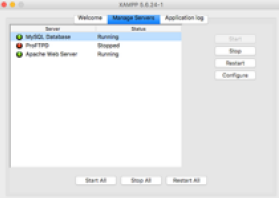
\includegraphics[scale=1]{figures/XAMPP.png}
\caption{Pannello di controllo XAMPP} 
\end{figure}
\end{center}

Avviati i server di Apache e MySQL (gli utenti Windows dovranno avviare anche Tomcat), è sufficiente collegarsi alla pagina: \url{http://localhost/dashboard/} e accedere alla pagina relativa alla voce \textit{\textbf{phpMyAdmin}} per gestire il proprio database. 

\begin{center}
\begin{figure}[H]
\centering
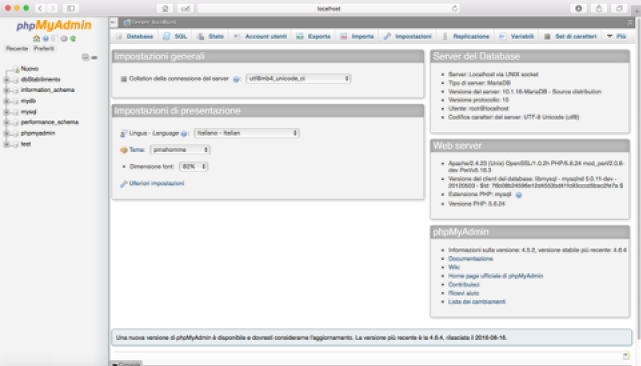
\includegraphics[scale=0.8]{figures/phpmyAdmin.png}
\caption{phpmyAdmin} 
\end{figure}
\end{center}

Si prende in considerazione lo scenario in cui uno o più clienti acquistano uno o più prodotti.

\begin{center}
\begin{figure}[H]
\centering
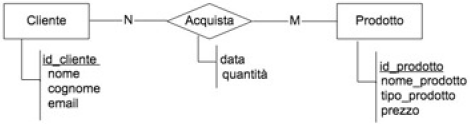
\includegraphics[scale=1]{figures/cbuyp4.png}
\caption{Cliente Acquista Prodotto} 
\end{figure}
\end{center}

Il precedente modello ER presenta due entità (Cliente e Prodotto) legate dalla relazione Acquista (cardinalità N:M). Entità e relazione sono caratterizzate dalla presenza di alcuni attributi; per poter identificare in modo univoco le entità si useranno le chiavi primarie (id\_cliente e id\_prodotto). Su tale scenario si crea il database su \textit{\textbf{phpMyAdmin}} direttamente cliccando sulla voce \textit{\textbf{Nuovo}} nella pagina iniziale e andando a specificare il nome e la codifica caratteri del database (si consiglia \textit{\textbf{utf8.general.ci}}, la quale permette l'uso di caratteri speciali ed è case insensitive). Fatto ciò vengono create le tabelle per le entità e la relazione. Ogni tabella sarà caratterizzata da un certo numero di colonne corrispondenti agli attributi, nelle quali si ha la possibilità di specificare informazioni quali il tipo, la lunghezza, la codifica e altro. 

\begin{center}
\begin{figure}[H]
\centering
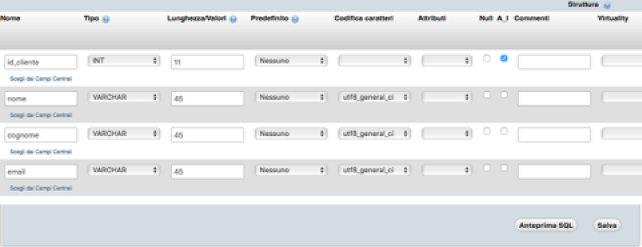
\includegraphics[scale=0.8]{figures/phpmyAdmin_table.png}
\caption{phpmyAdmin - Creazione tabella} 
\end{figure}
\end{center}

Una di queste prevede la specifica della chiave primaria per identificare univocamente ogni record della tabella; per farlo bisogna inserire il valore \textit{\textbf{primary}} nella sezione \textit{\textbf{Indice}} relativa all'attributo che si vuole usare come chiave.

\begin{center}
\begin{figure}[H]
\centering
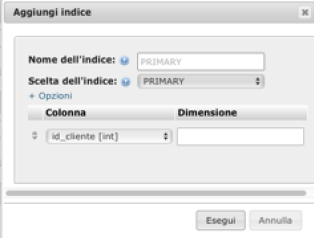
\includegraphics[scale=1]{figures/phpmyAdmin_addindex.png}
\caption{phpmyAdmin - Aggiungi indice} 
\end{figure}
\end{center}

Diversamente dall'entità, la relazione è priva di chiavi primarie in quanto è univocamente identificata dalle chiavi esterne. Per specificare le chiavi esterne bisogna selezionare la tabella relativa alla relazione e cliccare sulla voce \textit{\textbf{Relazione Vista}} per poi apportare le modifiche mostrate in figura indicando quale colonna usare come chiave esterna e in quale tabella è collocata.

\begin{center}
\begin{figure}[H]
\centering
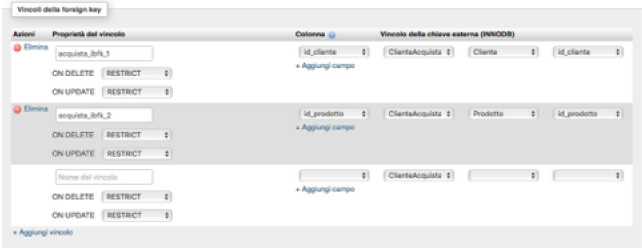
\includegraphics[scale=0.8]{figures/phpmyAdmin_foreignkey.png}
\caption{phpmyAdmin - Vincoli foreign key} 
\end{figure}
\end{center}

Una volta completate, le tabelle possono essere riempite cliccando sulla voce \textit{\textbf{Inserisci}} e compilando la seguente sezione.

\begin{center}
\begin{figure}[H]
\centering
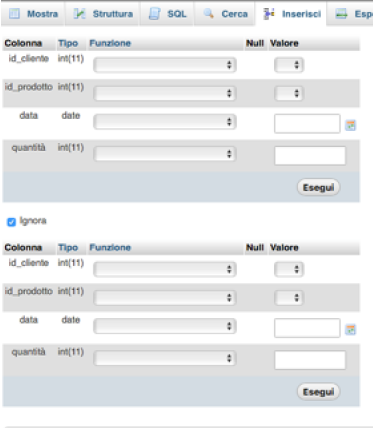
\includegraphics[scale=1]{figures/phpmyAdmin_addrecord.png}
\caption{phpmyAdmin - Aggiunta record} 
\end{figure}
\end{center}

Popolato il database, possiamo estrapolare il modello ER direttamente da \textit{\textbf{phpMyAdmin}} cliccando sulla voce \textit{\textbf{Designer}} nella barra degli strumenti dell'applicazione.

\begin{center}
\begin{figure}[H]
\centering
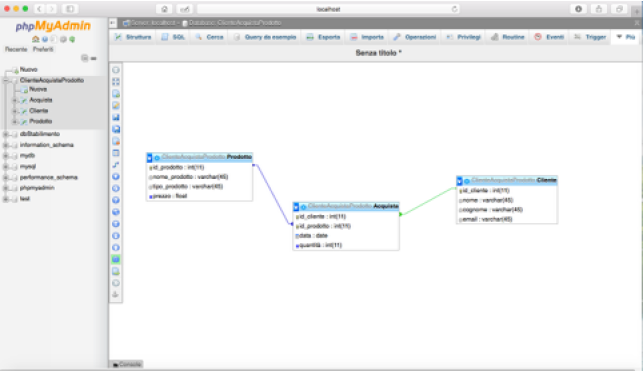
\includegraphics[scale=0.8]{figures/phpmyAdmin_designer.png}
\caption{phpmyAdmin - Modalità designer} 
\end{figure}
\end{center}

Si ha inoltre la possibilità di esportare tale modello in due modi:

\begin{itemize}

\item veloce, dove è possibile scegliere solo il formato (*.sql, *.csv, ...); \item personalizzato, dove oltre al formato, è possibile scegliere quali tabelle esportare, la codifica dei caratteri e altre opzioni aggiuntive.

\end{itemize}

Un'altra importante funzionalità di \textit{\textbf{phpMyAdmin}} è la realizzazione di query tramite la schermata messa a disposizione dall'applicazione o per mezzo della \textit{\textbf{visual builder}} che permette di costruire la query andando a scegliere graficamente gli attributi desiderati direttamente dal modello.

\begin{center}
\begin{figure}[H]
\centering
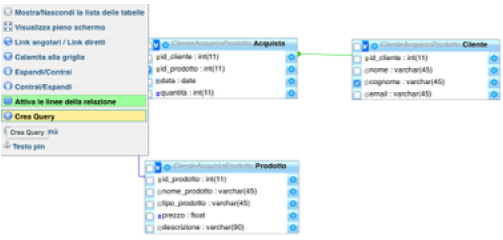
\includegraphics[scale=1]{figures/phpmyAdmin_visualbuilder.png}
\caption{phpmyAdmin - Visual Builder} 
\end{figure}
\end{center}

\begin{center}
\begin{figure}[H]
\centering
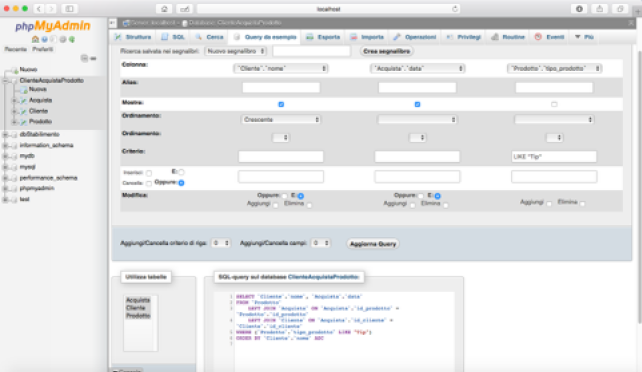
\includegraphics[scale=0.8]{figures/phpmyAdmin_query.png}
\caption{phpmyAdmin - Schermata query} 
\end{figure}
\end{center}

L'applicazione presenta altre funzionalità quali la scelta dei privilegi da attribuire ai diversi account oppure la possibilità di apportare modifiche al database o anche l'opportunità  di ottenere il dizionario dei dati in formato pdf.

\begin{center}
\begin{figure}[H]
\centering
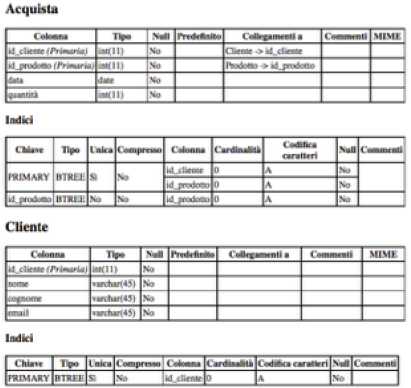
\includegraphics[scale=0.8]{figures/phpmyAdmin_tablerecap.png}
\caption{phpmyAdmin - Ricapitolazione tabella} 
\end{figure}
\end{center}


\subsection{MySQL Workbench}

MySQL Workbench è uno strumento visuale di progettazione per database che integra sviluppo SQL, gestione, modellazione dati, creazione e manutenzione di database MySQL all'interno di un unico ambiente. Il primo passo consiste nella creazione di una nuova connessione, specificandone il nome, il metodo di connessione e gli altri parametri richiesti.

\begin{center}
\begin{figure}[H]
\centering
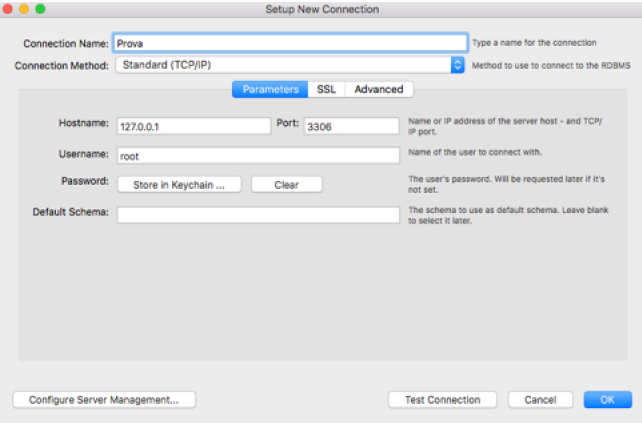
\includegraphics[scale=0.8]{figures/mySQL_workbench_newcon.png}
\caption{MySQL Workbench - New Connection} 
\end{figure}
\end{center}

Creata e aperta la connessione si ha la possibilità di ottenere informazioni su:

\begin{itemize}

\item management;
\item instance;
\item performance;
\item schemas. 

\end{itemize}

Dalla sezione \textit{\textbf{management}}, ad esempio, si può importare e/o esportare un database. Nella sezione \textit{\textbf{schemas}} troveremo tutti gli schemi creati, tra cui quello realizzato precedentemente con \textit{\textbf{phpMyAdmin}}. Selezionandolo è possibile gestire il proprio database, apportare delle modifiche, creare nuove tabelle o inserire dei record nelle tabelle presenti. 

\begin{center}
\begin{figure}[H]
\centering
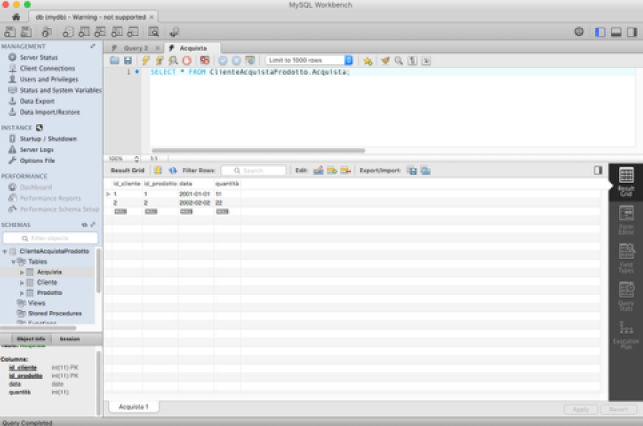
\includegraphics[scale=0.8]{figures/mySQL_workbench_query.png}
\caption{MySQL Workbench - Query} 
\end{figure}
\end{center}

Una funzionalità importante consiste nel creare il diagramma EER a partire dallo schema; per farlo è sufficiente selezionare lo schema desiderato e cliccare sulla voce \textit{\textbf{Reverse Engineering}} presente nel menu \textit{\textbf{Database}}.

\begin{center}
\begin{figure}[H]
\centering
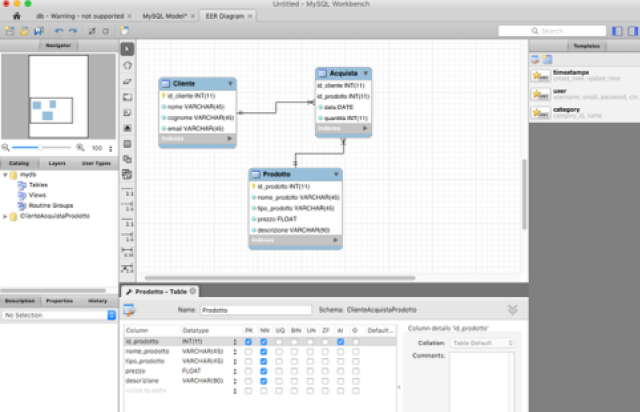
\includegraphics[scale=0.8]{figures/mySQL_workbench_reveng.png}
\caption{MySQL Workbench - Reverse Engineering} 
\end{figure}
\end{center}

Ottenuto il diagramma è possibile apportare delle modifiche  alle entità e agli attributi direttamente. Una volta modificato si ha la possibilità di sincronizzarlo con lo schema presente nel database tramite la voce \textit{\textbf{Synchronize Model}} nel menu \textit{\textbf{Database}}. Tramite questa funzionalità si modifica direttamente lo schema in modo da non avere difformità tra il diagramma EER e il database; l'applicazione notifica quale entità è stata modificata in modo da evitare errori e poi visualizza le query necessarie alle modifiche desiderate.

\begin{center}
\begin{figure}[H]
\centering
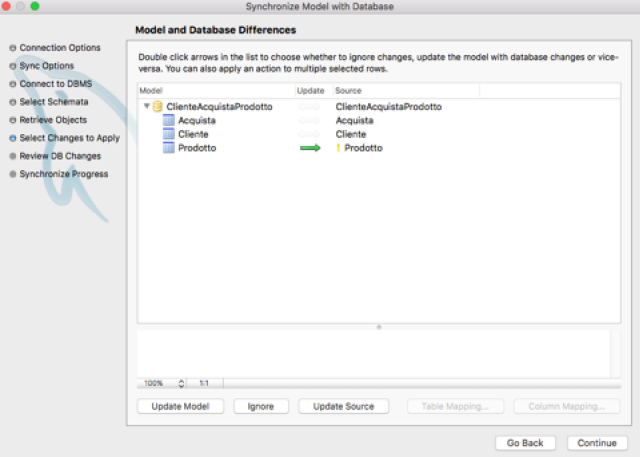
\includegraphics[scale=0.8]{figures/mySQL_workbench_synchmodel.png}
\caption{MySQL Workbench - Synchronize Model} 
\end{figure}
\end{center}


\subsection{DataGrip}

DataGrip è un IDE sviluppato da JetBrains che permette di:

\begin{itemize}

\item accedere ai principali DBMS;
\item modificare gli oggetti del database;
\item scrivere in modo facilitato del codice SQL;
\item eseguire query in modo facilitato. 

\end{itemize}

Una delle caratteristiche interessanti, rispetto ai DBMS precedenti, è la possibilità del confronto tra una specifica sottoquery ed una tabella per vedere le eventuali righe aggiuntive rispetto ad una query selezionata. Diversamente dagli altri editor, DATAGRIP permette l'autocompletamento ed eventuali suggerimenti nella trascrizione dei comandi SQL. A parte alcune funzionalità aggiuntive, presenta le stesse caratteristiche già viste in phpMyAdmin e MySQL Workbench.

\begin{center}
\begin{figure}[H]
\centering
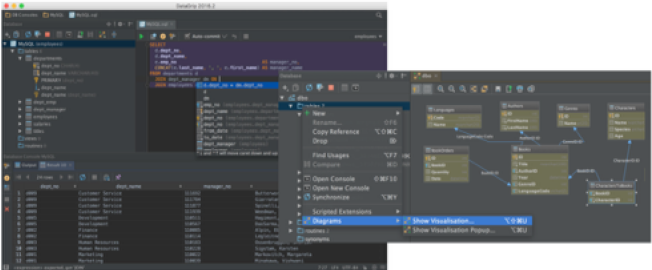
\includegraphics[scale=0.8]{figures/datagrip.png}
\caption{DataGrip} 
\end{figure}
\end{center}


\begin{flushright}Luca Signore\\Cristian Annicchiarico\\20/10/2016\end{flushright}


\section{Algebra Relazionale}

\subsection{INTRODUZIONE}

L’algebra relazionale è l’algebra su cui si basa il linguaggio SQL, cioè il linguaggio utilizzato per interrogare (to query) i databases. L’algebra relazionale opera su oggetti chiamati relazioni o tabelle, le quali sono sempre il risultato di un espressione, quindi di un insieme di oggetti e operatori. 

\begin{center}
\begin{figure}[H]
\centering
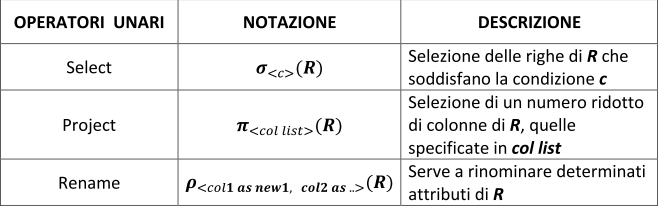
\includegraphics[scale=0.8]{figures/relalg.png}
\caption{Operatori Unari Algebra Relazionale} 
\end{figure}
\end{center}

Gli operatori binari, sono operatori che operano su insiemi, detti appunto \textit{SET THEORETICAL}; operano su oggetti \textit{Union-Compatible}, cioè su relazioni o tabelle con colonne dello stesso tipo (non necessariamente con colonne dello stesso nome).

\begin{center}
\begin{figure}[H]
\centering
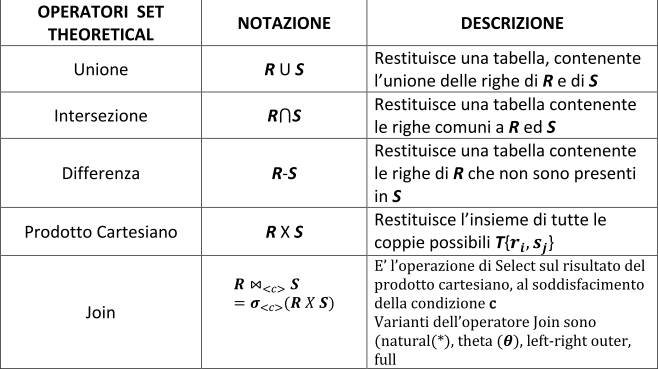
\includegraphics[scale=0.8]{figures/relalg2.png}
\caption{Operatori Binari Algebra Relazionale} 
\end{figure}
\end{center}

Il grado di selettività di una Join è un parametro importante di cui bisogna tener conto per migliorare ad esempio l’efficienza di un motore di ricerca. 

\subsection{ALTRI OPERATORI}

\begin{itemize}

\item{\textbf{Le funzioni di aggregazione}}

E’ una famiglia di operatori utilizzati per effettuare analisi statistiche sui dati:

\[
	<grouping\ attribute>\mathbf{F}<function\ list>(\mathbf{R})
\]

Questo operatore, raggruppa i records secondo il criterio di raggruppamento specificato nel \textit{grouping attribute} ed applica le funzioni specificate in \textit{function list}. Possibili scelte di \textit{function list} sono:

\begin{itemize}

\item{\textbf{Count}}: Conteggio;
\item{\textbf{Avg}}: Media;
\item{\textbf{Sum}}: Somma;
\item{\textbf{Max}}: Valore massimo;
\item{\textbf{Min}}: Valore minimo;
\item{\textbf{Var}}: Varianza;
\item{\textbf{Std Dev}}: Deviazione standard.

\end{itemize}

In linguaggio SQL: 

\begin{lstlisting}[language=SQL]
SELECT function list
FROM ...
WHERE ...
GROUP BY grouping attribute
HAVING ... -- condizioni sul risultato delle funzioni in function list 
\end{lstlisting}

\item{\textbf{Operatore di Divisione}}

Può essere considerato anch’esso un operatore di aggregazione, poiché, come per le funzioni di aggregazione, opera su più righe contemporaneamente. 

\[
	\mathbf{R} / \mathbf{S}
\]

Per spiegare bene come funziona, è utile osservare il seguente esempio: 

Consideriamo R come la composizione di due gruppi distinti di campi $(A,B)$, ed S come la composizione di uno solo dei due gruppi di R: $\implies R/S := T$:

\begin{center}
\begin{figure}[H]
\centering
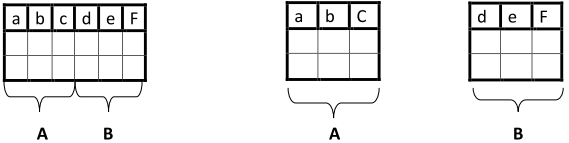
\includegraphics[scale=0.8]{figures/division.png}
\caption{Operatore Divisione} 
\end{figure}
\end{center}

In altre parole, come visto nell’esempio di prima, l’operatore diviso restituisce una tabella con solo le colonne di \textit{\textbf{R}} che non sono in \textit{\textbf{S}}.

\end{itemize}

L’insieme degli operatori visti finora  è completo, poiché con esso si può interrogare il database in qualsiasi modo possibile, allo scopo di reperire tutte le informazioni di cui necessitiamo, se presenti. Il caso senz’altro più difficile da gestire è quello della chiusura ricorsiva, poiché gli operatori di cui abbiamo discusso consentono di interrogare il Database in tutti i modi finiti possibili, cioè solo nei casi in cui si ha una conoscenza a priori del numero di iterazioni di una data struttura. 
A titolo di esempio, supponiamo di dover creare un database contenente un albero genealogico: 

\begin{center}
\begin{figure}[H]
\centering
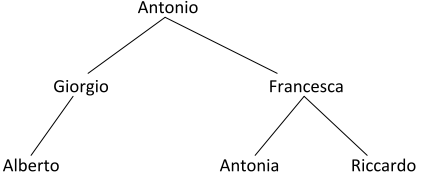
\includegraphics[scale=1]{figures/gen_tree.png}
\caption{Albero genealogico} 
\end{figure}
\end{center}

Il corrispondente modello ER e relativo modello relazionale, sono i seguenti:  

\begin{center}
\begin{figure}[H]
\centering
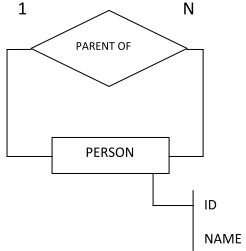
\includegraphics[scale=1]{figures/parent_of.png}
\caption{ER della relazione Parent Of} 
\end{figure}
\end{center}

\begin{center}
\begin{figure}[H]
\centering
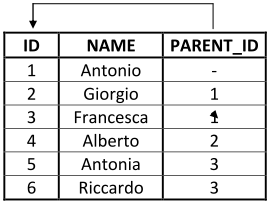
\includegraphics[scale=1]{figures/parent_of_relational.png}
\caption{Modello relazionale della relazione Parent Of} 
\end{figure}
\end{center}

E’ possibile vedere gli zii? Basta trovare il genitore di x e vedere i suoi fratelli. 
Applicando il prodotto cartesiano e poi applicando il vincolo di integrità referenziale nella join $(<PARENT\_ID=ID>)$, ottengo: 

\begin{center}
\begin{figure}[H]
\centering
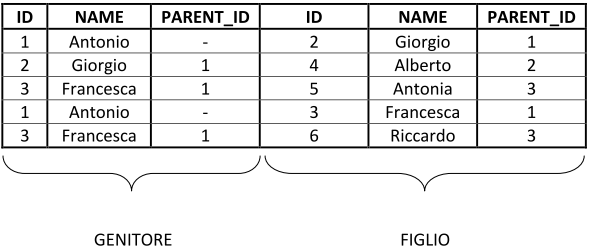
\includegraphics[scale=0.8]{figures/genitore_join_figlio.png}
\caption{Genitore JOIN Figlio} 
\end{figure}
\end{center}
	
Successivamente, per controllare se il genitore di x ha fratelli, applico nuovamente l’operatore di Join. 
Questo esempio, spiega allora come non sia possibile trovare tutti i figli di un progenitore in “un colpo solo” a meno che non si conosca il numero di livelli di un albero.  


\subsection{ESEMPI DI QUERY}

\begin{center}
\begin{figure}[H]
\centering
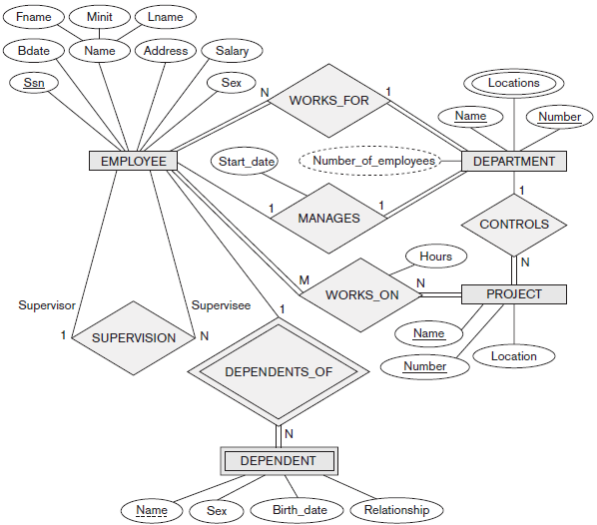
\includegraphics[scale=0.7]{figures/tcd2.png}
\caption{The Company Database} 
\end{figure}
\end{center}

\begin{itemize}

\item{\underline{\textbf{QUERY 1}}}: \textit{Nome e indirizzo di tutti gli impiegati che lavorano per il dipartimento di nome “Research”}:

\[
	\pi_{<Name,Address>}(\sigma_{DEPARTMENT.Name='Research'}(
\]
\[
	DEPARTMENT \Join_{<DEPARTMENT.number=EMPLOYEE.DEP\_no>} EMPLOYEE))
\]

È necessario effettare un’\textbf{inner join} tra Department ed Employee, selezionare con una \textbf{select} le righe in cui l’attributo Name vale “Research”, e fare una \textbf{project} per ottenere soltanto le colonne Name ed Address. 

\textbf{n.b.} sul testo la query è suddivisa in tre passaggi, per una maggiore chiarezza. Essi, però, non sono eseguiti in momenti distinti, ma in un unico blocco, come riportato sopra. 
La versione SQL della stessa query è:

\begin{lstlisting}[language=SQL]
SELECT Employee.Name, Employee.Address 
FROM Employee JOIN Department ON Department.number=Employee.Dep_no 
WHERE Department.Name="Research"
\end{lstlisting}

\item{\underline{\textbf{QUERY 2}}}: \textit{Per ogni progetto situato a Lecce, elencare il project number, il controlling department number e il nome del direttore che controlla il dipartimento}.

Le tabelle coinvolte sono Department, Employee e Project. Nel modello relazionale, il numero di dipartimento diventa attributo chiave esterna nella tabella Project (perché CONTROLS è una relazione 1:N nel modello ER). Assumiamo, inoltre, che la relazione Employee-MANAGES Department sia inclusa lato Department (l’ssn del direttore del dipartimento diventa attributo chiave esterna nella tabella Department). La query in SQL risulta essere la seguente: 

\begin{lstlisting}[language=SQL]
SELECT Project.Number, Project.Dep_Number, Employee.Name 
FROM (Project JOIN Department ON Department.Number=Project.Dep_Number)
			  JOIN Employee ON Department.employee_ssn=Employee.Ssn 
WHERE Project.Location="Lecce"
\end{lstlisting}

\end{itemize}


\begin{flushright}Marco D'Amato\\Adriano Luigi Piscopello\\26/10/2016\end{flushright}


\section{Queries}

L’insieme degli operatori fondamentali dell’algebra relazionale è composto da operatori associativi e non associativi, quest’ultimi agiscono su una singola entità, (selezione di determinate tuple, di particolari attributi ecc) mentre i primi operano su più entità diverse.  

Le \textbf{operazioni associative} sono alla base della nostra stessa memoria, infatti queste hanno il compito di mettere insieme diverse entità, in modo da cercare degli elementi in base a dei criteri prestabiliti. Un esempio potrebbe essere quello di cercare tutti i frequentanti di un corso che hanno i capelli lunghi. 
 
Gli \textbf{operatori associativi} li possiamo associare alle funzioni di aggregazione e la divisione.  

Le \textbf{funzioni di aggregazione} permettono, come dice il nome stesso, di aggregare più informazioni in una sola, ad esempio possiamo vedere quanti impiegati ci sono in un’azienda, senza voler prendere il nome di ognuno. Questi operatori ci permettono di effettuare qualsiasi query sul database (possiamo estrarre qualsiasi informazione dal database, se presente, escluso il caso di recursive closure). Facciamo un esempio pratico, partendo da un database studiato precedentemente: Il “Company” Database.   

\begin{center}
\begin{figure}[H]
\centering
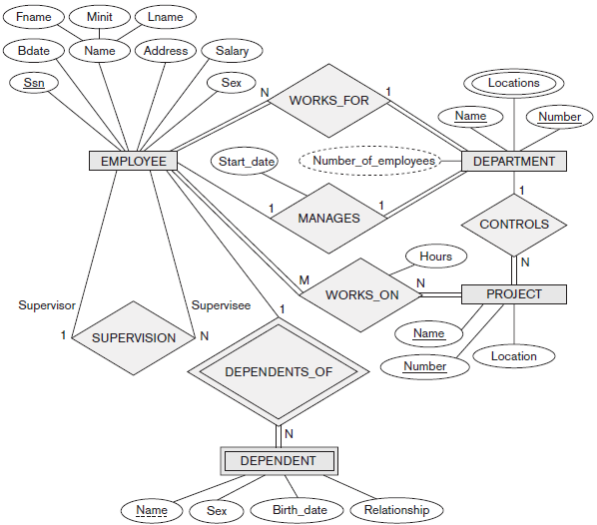
\includegraphics[scale=0.7]{figures/tcd2.png}
\caption{The Company Database} 
\end{figure}
\end{center}

Attraverso le conoscenze pregresse, riusciamo a estrarre mentalmente quali saranno le tabelle che avremo sul database guardando direttamente il modello concettuale.  
L’entità \textit{department} ha un attributo multiplo \textit{locations}. Questo attributo, che nel modello logico diverrà una \textbf{weak entity type}, avrà una relazione \textit{department has location} con cardinalità 1 a n. Questa trasformazione si può effettuare per qualsiasi attributo multiplo o composto del modello ER. Nella trasformazione tra modello ER a modello logico si ha un problema comune:  Qual è la primary key?  Nella tabella \textit{department}, nel caso di diagramma ER, le primary keys saranno \textit{name} e \textit{number}. Queste a livello logico dovranno essere sostituite da una primary key numerica per ottimizzare le \textbf{join}, mentre, sempre a questo livello, gli attributi name e number dovranno essere inseriti come normali attributi imponendo, se necessario, le condizioni di \textbf{NOT NULL} e \textbf{UNIQUE}. Queste particolari trasformazioni permettono di sfruttare la \textit{\textbf{gestione dei sospesi}}: possiamo inserire tutti i dati senza la chiave primaria concettuale, per poi rimanere in sospeso fino a quando non decidiamo di chiuderla e salvarla sul database.  

Tornando al nostro esempio, dal diagramma ER possiamo vedere che la relazione \textit{employee-manages-department} ha cardinalità 1 a 1, quindi possiamo mettere la chiave primaria di “\textit{employee}” come chiave esterna a \textit{department} (director\_id). Per la relazione \textit{employee-works\_for-department}, possiamo notare che ha cardinalità n a 1, quindi dobbiamo inserire la chiave primaria di department come chiave esterna in \textit{employee} (department\_id). Come detto precedentemente, dobbiamo creare la tabella \textit{location} e, avendo la relazione n a 1 con \textit{department}, dobbiamo aggiungere la chiave esterna \textit{department\_id} alla tabella \textit{location}. L’entità \textit{project} diventa una tabella con id, tutti gli altri attributi e la chiave esterna al dipartimento associato (department\_id). La relazione \textit{employee-works\_on-project} è n a m, quindi si crea una nuova tabella con le chiavi esterne (primarie) che puntano alle tabelle a cui è associata (employee\_id, project\_id) e gli attributi aggiuntivi (hours). Per la relazione \textit{employee-supervisions-employee}, aggiungiamo un attributo chiave esterna alla tabella \textit{employee} (supervisioner\_id) in riferimento alla tabella \textit{employee} stessa. 
 
Proviamo a risolvere i seguenti esercizi tramite l’utilizzo di queries. Si noti che l’utilizzo di più queries per la risoluzione di un singolo problema è puramente per motivi di spazio e leggibilità. 

\begin{center}
\begin{figure}[H]
\centering
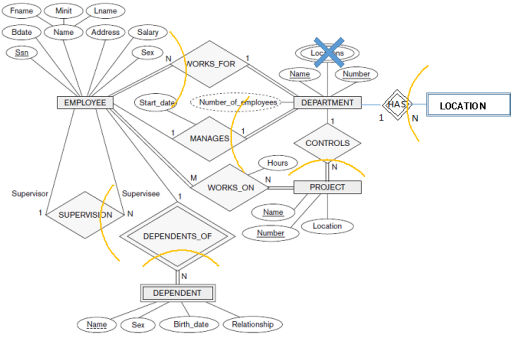
\includegraphics[scale=0.8]{figures/tcdmod.png}
\caption{The Company Database - Logical Mapping Inclusions} 
\end{figure}
\end{center}

\begin{center}
\begin{figure}[H]
\centering
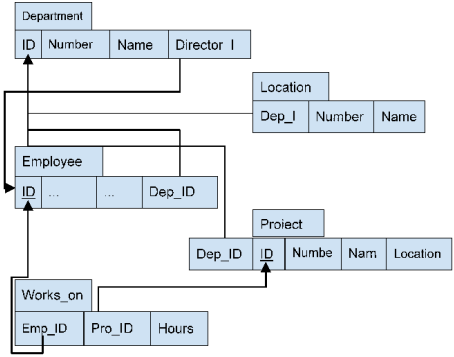
\includegraphics[scale=1]{figures/tcd_logical.png}
\caption{The Company Database - Logical} 
\end{figure}
\end{center}


\begin{itemize}

\item{\textbf{Query 1}}: \textit{Restituire il nome e l’indirizzo di ogni impiegato che lavora per il dipartimento “ricerca”}.

\[	
	\pi_{<name,address>}(employees \Join_{<e.depId=d.id>}\sigma_{<name="research">}(department))
\]

\begin{itemize}

\item Estraiamo tramite l’operazione di \textbf{select}, i dipartimenti che hanno nome “ricerca”;
\item Il risultato ottenuto verrà unito, tramite comando \textbf{join}, alla tabella \textit{employee} col vincolo di chiave esterna (employee.dep\_id = department.id);
\item A quest’ultimo risultato verrà applicata una \textbf{projection} sui campi \textit{name} e \textit{address}, per estrarre solo questi attributi.

\end{itemize}

\item{\textbf{Query 2}}: \textit{Trovare i nomi degli impiegati che lavorano per tutti i progetti controllati dal dipartimento numero 5}.

\[	
	\left\{
	\begin{aligned}
	&DEPT5\_PROJS \leftarrow \rho_{(Pno)}(\pi_{<Pnumber>}(\sigma_{<Dnum=5>}(project)))\\
	&EMP\_PROJ \leftarrow \rho_{(Ssn,Pno)}(\pi_{<Essn,Pno>}(works\_on))\\
	&RESULT\_EMP\_SSNS \leftarrow EMP\_PROJ / DEPT5\_PROJS\\
	&RESULT \leftarrow \pi_{<Lname,Fname>}(RESULT\_EMP\_SSNS * employee)
	\end{aligned}
	\right.
\]

\begin{itemize}

\item Estraiamo i progetti con numero di dipartimento = 5 e rinominiamo l’attributo project\_number in \textit{Pno};
\item Estraiamo l’ssn e il project\_number dalla tabella \textit{works\_on};
\item Dividiamo il risultato della seconda query per il risultato della prima per avere l’ssn dei dipendenti che lavorano su TUTTI i progetti del dipartimento 5;
\item Facciamo una \textbf{join} con la tabella \textit{employee} per restituire nome e cognome dei dipendenti richiesti.  

\end{itemize}


\item{\textbf{Query 4}}: \textit{Creare una lista di progetti che hanno almeno un impiegato di cognome “Smith”, o come lavoratore o come manager del dipartimento che controlla il progetto}.

\[
	\left\{
	\begin{aligned}
	&SMITHS(Essn) \leftarrow \pi_{<Essn>}(\sigma_{<Lname="Smith">}(employee))\\
	&SMITH\_WORKER\_PROJS \leftarrow \pi_{<Pno>}(works\_on * SMITHS)\\
	&MGRS \leftarrow \pi_{<Lname,Dnumber>}(employee \Join_{<ssn=mgrSsn>}department)\\
	&SMITH\_MANAGED\_DEPTS(Dnum) \leftarrow \pi_{<Dnumber>}(\sigma_{<Lname="Smith">}(MGRS))\\
	&\left[
	\begin{aligned}
	&SMITH\_MGR\_PROJS(Pno) \leftarrow\\
	&\leftarrow \pi_{<Pnumber>}(SMITH\_MANAGED\_DEPTS * project)
	\end{aligned}
	\right.\\
	&RESULT \leftarrow (SMITH\_WORKER\_PROJS \cup SMITH\_MGR\_PROJS)
	\end{aligned}
	\right.
\]

\begin{itemize}

\item Restituiamo il valore degli ssn dei dipendenti di cognome “Smith” tramite select e \textbf{projection};
\item Troviamo gli id dei progetti in cui lavorano impiegati di nome “Smith” (trovato dalla query precedente);
\item Restituiamo il nome dei manager dei vari dipartimenti con il corrispettivo numero di dipartimento;
\item Selezioniamo gli ssn degli impiegati col cognome “Smith” dalla query precedente;
\item Troviamo il numero dei progetti associati ai dipartimenti restituiti dalla query precedente;
\item Uniamo i risultati della seconda e della quinta query. 

\end{itemize}

\item{\textbf{Query 5}}: \textit{Lista dei nomi di tutti gli impiegati con 2 o più parenti a carico}.

\[
	\pi_{<Lname,Fname>}(\sigma_{<count\geq 2>}(_{ssn}F_{COUNT\ name}(dependent))*employee)
\]

\begin{itemize}

\item Contiamo il numero di familiari a carico presenti per ogni ssn degli impiegati (utilizzando l’apposita funzione di aggregazione \textit{\textbf{COUNT}});
\item Selezioniamo tramite \textbf{select} gli ssn che hanno $count\geq 2$;
\item Il risultato verrà unito tramite \textbf{join} alla tabella \textit{employee} per restituire il nome e il cognome degli impiegati richiesti.

\end{itemize}

\item{\textbf{Query 6}}: \textit{Restituire i nomi dei dipendenti che non hanno parenti a carico}.

\[
	\left\{
	\begin{aligned}
	&ALL\_EMPS \leftarrow \pi_{Ssn}(employee)\\
	&EMPS\_WITH\_DEPS(Ssn) \leftarrow \pi_{Essn}(dependent)\\
	&EMPS\_WITHOUT\_DEPS(Ssn) \leftarrow (ALL\_EMPS - EMPS\_WITH\_DEPS)\\
	&RESULT \leftarrow \pi_{Lname,Fname}(EMPS\_WITHOUT\_DEPS * employee)
	\end{aligned}
	\right.
\]

\begin{itemize}

\item Estraiamo la lista di ssn degli impiegati;
\item Estraiamo la lista di ssn degli impiegati con familiari a carico;
\item Sottraiamo il primo risultato col secondo;
\item Restituiamo, tramite \textbf{join} con la tabella \textit{employee}, il nome e il cognome dei dipendenti rimasti. 

\end{itemize}

\item{\textbf{Query 7}}: \textit{Restituire il nome dei manager che hanno un familiare a carico}.

\[
	\left\{
	\begin{aligned}
	&MGRS(Ssn) \leftarrow \pi_{MgrSsn}(department)\\
	&EMPS\_WITH\_DEPS(Ssn) \leftarrow \pi_{Essn}(dependent)\\
	&MGRS\_WITH\_DEPS \leftarrow (MGRS \cap EMPS\_WITH\_DEPS)\\
	&RESULT \leftarrow \pi_{Lname,Fname}(MGRS\_WITH\_DEPS * employee)
	\end{aligned}
	\right.
\]

\begin{itemize}

\item Estraiamo l’elenco degli ssn dei managers dei dipartimenti;
\item Estraiamo l’elenco degli ssn degli impiegati con familiari a carico;
\item Intersechiamo i due risultati precedenti per restituire gli ssn dei manager con familiari a carico;
\item Troviamo il nome e il cognome dei managers calcolati precedentemente tramite join alla tabella employee. 

\end{itemize}

\end{itemize}


\begin{flushright}Emanuele Costa Cesari\\Paolo Panarese\\27/10/2016\end{flushright}


\section{Popolazione casuale DB}

Lo scopo della lezione è quello di andare a riempiere un database con dei dati casuali. 
I database sono principalmente di due categorie: 

\begin{itemize}
\item MYISAM 
\item INNODB
\end{itemize}

\begin{itemize}

\item{\textbf{MyISAM}} non utilizza le chiavi esterne nelle sue relazioni e non esistono le transazioni ma ha il vantaggio di essere molto veloce, inoltre, ogni tipo di dato viene rappresentato attraverso 3 diversi file: 

\begin{itemize}

\item{.frm} $\rightarrow$ dove viene rappresentata la parte strutturale;
\item{.myd} $\rightarrow$ dove vengono salvati i dati;
\item{.myi} $\rightarrow$ dove vengono salvati gli indici relativi alla tabella  
INNODB.

\end{itemize}

\item{\textbf{INNODB}} utilizza delle tabelle più complete ma allo stesso tempo più lente, però al contrario di MyISAM permette l’utilizzo di chiavi esterne e transazioni (commit e rollback).

\end{itemize}

Le Transazioni sono delle operazioni  atomiche che vengono eseguite sul DB come per esempio un bonifico, l’acquisto di un biglietto ecc. per default tutti gli aggiornamenti sono istantanei durante le transazioni, per evitare l’aggiornamento automatico bisogna cambiare il valore di AUTOCOMMIT. 

Nella creazione del DB ci troveremo ad avere delle tabelle in cui saranno presenti delle chiavi esterne, ciò che succede quando una tupla relativa ad una chiave esterna viene cancellata deve essere impostato durante la creazione del database utilizzando la clausola ON DELETE seguita da uno dei seguenti valori: 

\begin{itemize}

\item{CASCADE}: viene cancellata anche la tupla della tabella in cui è presente la chiave esterna;
\item{SET NULL} viene impostato il valore della chiave esterna a NULL;
\item{SET DEFAULT}: viene impostato il valore della chiave esterna al valore di default impostato;
\item{RESTRICT/NO ACTION}: si verifica prima o dopo aver tentato di aggiornare la casella.

\end{itemize}

\subsection{Tipi di dato in MySQL}

\begin{itemize}

\item{Numerici}: 

\begin{itemize}

\item BIT[(M)];
\item TINYINT[(M)] [UNSIGNED] [ZEROFILL];
\item SMALLINT[(M)] [UNSIGNED] [ZEROFILL];
\item MEDIUMINT[(M)] [UNSIGNED] [ZEROFILL];
\item INT[(M)] [UNSIGNED] [ZEROFILL];
\item BIGINT[(M)] [UNSIGNED] [ZEROFILL];
\item FLOAT[(M,D)] [UNSIGNED] [ZEROFILL];
\item DOUBLE[(M,D)] [UNSIGNED] [ZEROFILL];
\item DECIMAL[(M[,D])] [UNSIGNED] [ZEROFILL]

\end{itemize}

\item{Alfanumerici}:

\begin{itemize}

\item{} [NATIONAL] CHAR(M) [BINARY | ASCII | UNICODE];
\item{} [NATIONAL] VARCHAR(M) [BINARY];
\item BINARY(M);
\item VARBINARY(M);
\item TINYBLOB;
\item TINYTEXT;
\item BLOB[(M)];
\item TEXT[(M)];
\item MEDIUMBLOB;
\item MEDIUMTEXT;
\item LONGBLOB;
\item LONGTEXT;
\item ENUM('valore1','valore2', \dots);
\item SET('valore1','valore2', \dots)

\end{itemize}

\item{Date e tempo}:

\begin{itemize}

\item DATE;
\item DATETIME;
\item TIMESTAMP[(M)];
\item TIME - YEAR[(2|4)] 

\end{itemize}

\end{itemize}

\subsection{Attributi}

Oltre ad impostare il valore di ogni colonna possiamo impostare altri valori tra cui:

\begin{itemize}

\item{Primary Key}: rappresenta quale campo viene usato come chiave primaria nella tabella, deve essere necessariamente unica e usando l’attributo AUTOINCREMENT viene incrementata automaticamente ad ogni inserimento usando il primo valore libero;
\item{UNIQUE}: può essere impostato anche se il campo non è una chiave primaria e richiede che ogni valore sia diverso dagli altri;
\item{INDEX}: velocizza l’accesso ai dati generando degli indici, a differenza della PRIMARY KEY non è un valore unico.

\end{itemize}

\subsection{Funzioni di Aggregazione}

La clausola GROUP BY serve a specificare quali sono i campi sui cui effettuare i raggruppamenti: il motore di query, per ogni riga esaminerà tali campi e la classificherà nel gruppo corrispondente. Si possono specificare calcoli da effettuare per ogni gruppo. Esempi di operazioni sono:

\begin{itemize}

\item{DISTINCT}: visualizza solo valori distinti nel raggruppamento;
\item{COUNT(*)}: conta il numero di occorrenze nel raggruppamento;
\item{AVG}: calcola la media dei valori;
\item{SUM}: somma i valori del raggruppamento. 

\end{itemize}

Con la clausola HAVING possiamo imporre delle condizioni ai soli raggruppamenti e ai soli campi per cui è stata utilizzata la clausola GROUP BY.

\subsection{Popolazione del DataBase}

\begin{itemize}

\item Creare nel DB la tabella che si vuole riempire. Nel nostro caso, usiamo una tabella di esempio, Persona, con gli attributi che si vedono nella figura. 

\begin{center}
\begin{figure}[H]
\centering
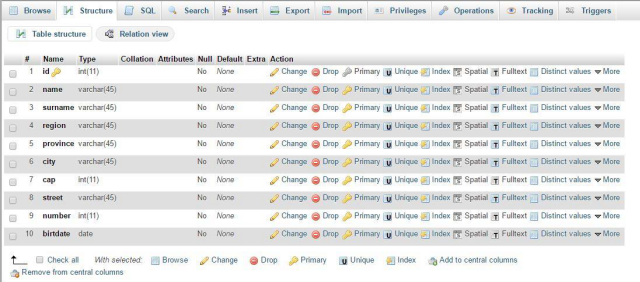
\includegraphics[scale=0.8]{figures/example_table.png}
\caption{phpmyAdmin - Tabella di esempio} 
\end{figure}
\end{center}

\item Creare un novo foglio, in Excel, in cui andremo a generare i valori casuali da inserire nel DB. 

\begin{center}
\begin{figure}[H]
\centering
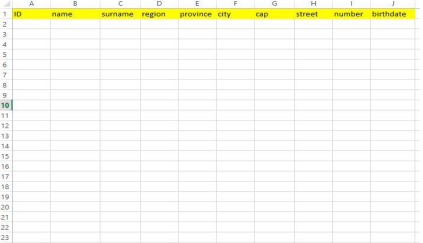
\includegraphics[scale=1]{figures/excel.png}
\caption{Microsoft Excel - Foglio di lavoro} 
\end{figure}
\end{center}

\item  Fare il download delle seguenti liste:

\begin{itemize}

\item Lista nomi italiani: \url{https://gist.github.com/pdesterlich/2562329};
\item Lista cognomi italiani: \url{https://gist.github.com/pdesterlich/2562407};
\item Lista comuni italiani, con relativi CAP, province e regioni: \newline\url{http://lab.comuni-italiani.it/download/comuni.html} (Quest’ultimo file è in formato CSV, quindi si può aprire con Excel).

\end{itemize}

\item Importare nel nostro file Excel, le liste sopraelencate:

\begin{center}
\begin{figure}[H]
\centering
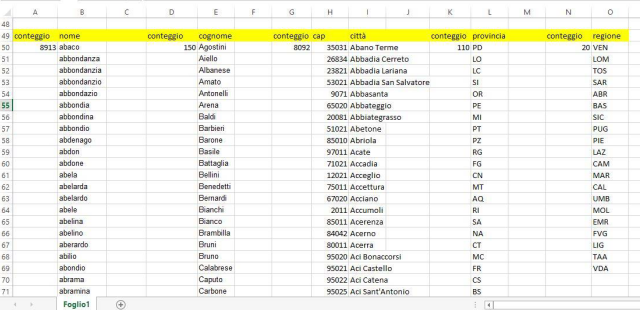
\includegraphics[scale=0.8]{figures/list_import_excel.png}
\caption{Microsoft Excel - Importazione liste} 
\end{figure}
\end{center}

Nelle celle A, D, G, K, N, c’è il numero totale di elementi delle liste che si trovano nelle colonne successive a quelle indicate.

\item Premere Alt + F11 per aprire la finestra che permette di implementare le nostre funzioni per generare i dati casuali.  

\item Cliccare con il tasto destro nella sezione indicata e selezionare inserisci modulo:

\begin{center}
\begin{figure}[H]
\centering
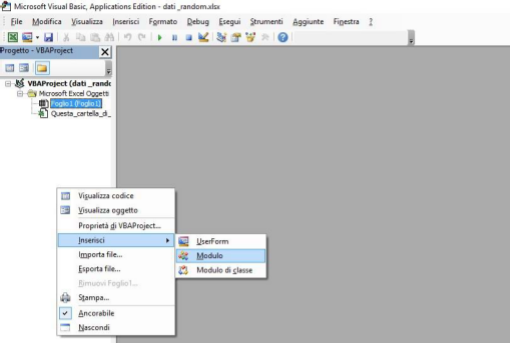
\includegraphics[scale=1]{figures/excel_VBA.png}
\caption{Microsoft Excel - Visual Basic for Applications} 
\end{figure}
\end{center}

\item Una volta creato il nuovo modulo, è possibile implementare le nostre funzioni per la generazione di dati casuali:

\begin{center}
\begin{figure}[H]
\centering
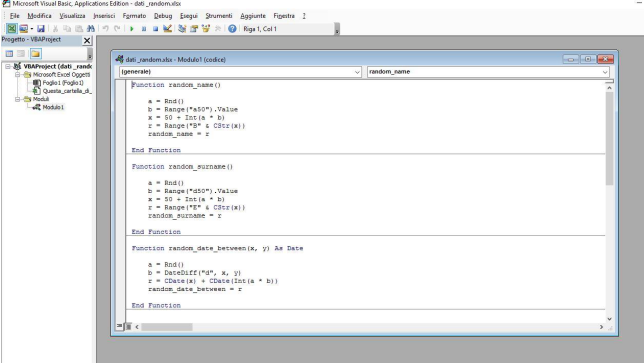
\includegraphics[scale=0.8]{figures/VBA.png}
\caption{Visual Basic for Applications - Nuovo Modulo} 
\end{figure}
\end{center}

Nel nostro caso abbiamo bisogno delle seguenti funzioni: 

\begin{lstlisting}[language={[Visual]Basic}]
Function random_name()  
	a = Rnd()
	b = Range("a50").Value
	x = 50 + Int(a * b)
	r = Range("B" & CStr(x))
	random_name = r  
End Function  

Function random_surname()  
    a = Rnd()    
    b = Range("d50").Value    
    x = 50 + Int(a * b)   
    r = Range("E" & CStr(x))    
    random_surname = r  
End Function  

Function random_date_between(x, y) As Date         
	a = Rnd()    
	b = DateDiff("d", x, y)    
	r = CDate(x) + CDate(Int(a * b))   
	random_date_between = r     
End Function  

Function cap(x)
	i = 50 For Each c In [i50:i8141]    
		If c.Value = x.Value Then
			y = i
	i = i + 1
	Next
	cap = Range("h" & CStr(y)).Value  
End Function 
     
Function random_city()  
    a = Rnd()    
    b = Range("g50").Value    
    x = 50 + Int(a * b)    
    r = Range("i" & CStr(x))    
    random_city = r  
End Function  

Function random_region()  
    a = Rnd()    
    b = Range("n50").Value   
    x = 50 + Int(a * b)    
    r = Range("o" & CStr(x))    
    random_region = r  
End Function 
 
Function random_province()  
    a = Rnd()    
    b = Range("k50").Value    
    x = 50 + Int(a * b)    
    r = Range("l" & CStr(x))    
    random_province = r  
End Function

\end{lstlisting}

\textbf{Bisogna fare attenzione agli indici delle celle utilizzati, se le liste sono state inserite in una posizione differente, è necessario aggiornare gli indici nelle funzioni che sono scritte sopra}.

\item  A questo punto è sufficiente utilizzare in Excel, le funzioni appena implementate per generare i dati.  

\begin{center}
\begin{figure}[H]
\centering
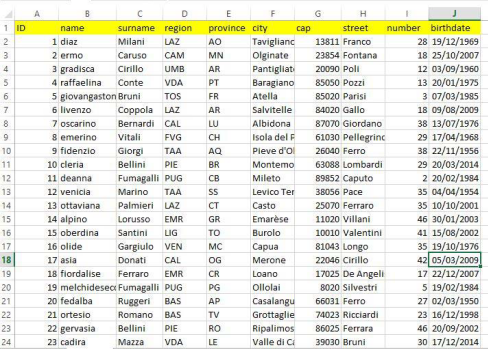
\includegraphics[scale=1]{figures/excel_populated.png}
\caption{Microsoft Excel - Tabella popolata} 
\end{figure}
\end{center}

\begin{itemize}

\item In B $\rightarrow F(x) =random\_name()$;
\item In C $\rightarrow F(x) =random\_surname()$;
\item In D $\rightarrow F(x) =random\_region()$;
\item In E $\rightarrow F(x) =random\_province()$;
\item In F $\rightarrow F(x) =random\_city()$;
\item In G $\rightarrow F(x) =cap(x)$;
\item In H $\rightarrow F(x) =random\_surname()$;
\item In I $\rightarrow F(x) =CASUALE.TRA(1;50)$;
\item In J $\rightarrow F(x) =random\_date\_between("01/01/1950";"01/01/2016")$. 

\end{itemize}

\end{itemize}


\begin{flushright}Lorenzo Caputo\\Mattia Marzano\\27/10/2016\end{flushright}


\section{MySQL}

\begin{itemize}

\item Tipi di tabelle (motori MyISAM e InnoDB);
\item Tipi di dati (numerici, alfanumerici, temporali):

\begin{itemize}
\item Con particolare attenzione alla gestione delle date;
\end{itemize}

\item Funzioni di aggregazione:

\begin{itemize}

\item MIN;
\item MAX;
\item AVG;
\item SUM;
\item \dots.

\end{itemize}

\item Indici.

\end{itemize}

In un DBMS in generale e in MySQL in particolare, i dati sono organizzati in:

\begin{itemize}

\item Database;
\item Tabelle.

\end{itemize}

\subsection{Tipi di tabelle}

I tipi di tabelle (o \textit{storage engine}) sono dei moduli software che si occupano della memorizzazione e del recupero delle informazioni.
 
\begin{itemize}

\item{\textbf{MyISAM}} (motore di default dalla versione 3.23 fino alla 5.1);
\item{\textbf{InnoDB}} (motore di default a partire dalla versione 5.0).

\end{itemize}

\subsubsection{MyISAM}

\begin{itemize}

\item Tabelle storiche di MySQL;
\item Garantiscono un’ottima affidabilità e velocità;
\item Vantaggio: la possibilità di poter utilizzare indici FULLTEXT per ricerche con ranking stile Google;
\item Mancano però di alcune caratteristiche molto importanti nelle basi di dati:

\begin{itemize}
\item Supporto alle chiavi esterne per garantire l’integrità referenziale;
\item Supporto alle transazioni;
\end{itemize}

\item Non sono adatte per realizzare sistemi di commercio elettronico o altre applicazioni enterprise;
\item Il metodo di salvataggio dei dati è basato sulla costruzione e lavorazione di 3 file binari per ogni tabella:

\begin{itemize}
\item nome\_tabella.frm: struttura della tabella (dimensioni e tipo di ogni colonna, indici, ...);
\item nome\_tabella.MYD: file che contiene tutti i dati della tabella;
\item nome\_tabella.MYI: file che contiene i dati relativi agli indici del database;
\end{itemize}

\item Per trasferire/copiare una o più tabelle da una macchina all’altra o da un database a un altro è sufficiente spostare questi 3 file $\rightarrow$ backup semplice;
\item Si affida al sistema operativo per il caching di letture e scritture sulle tabelle.

\end{itemize}

Le tabelle possono avere un formato:

\begin{itemize}

\item{\textbf{Statico}}: (quando la tabella non contiene colonne a lunghezza variabile es. varchar; offre maggiore sicurezza e velocità ma richiede più spazio sul disco);
\item{\textbf{Dinamico}}: (quando la tabella contiene colonne a lunghezza variabile; può però portare a una frammentazione della tabella) $\rightarrow$ è bene effettuare periodicamente un’ottimizzazione con il comando \textit{OPTIMIZE TABLE};
\item{\textbf{Compresso}}:  (utile per generare tabella a sola lettura che minimizzano l’occupazione di spazio; compressione con l’utility \textit{myisampack} e decompressione con l’utility \textit{myisamchk})

\end{itemize}

\subsubsection{InnoDB}

\begin{itemize}

\item Tabelle molto più complete delle MyISAM ma più lente a causa delle funzionalità aggiuntive di cui dispongono;
\item Vantaggi:

\begin{itemize}

\item Supporto per le chiavi esterne (\textit{foreign key}):
\begin{itemize}
\item Le tabelle sono in grado di gestire l’integrità referenziale tra le chiavi esterne del database;
\end{itemize}
\item Supporto per la transazionalità (fondamentale per le applicazioni di commercio elettronico in cui, finché non arriva conferma da parte della banca o di chi valida la carta di credito, le query non devono essere “eseguite realmente”):

\begin{itemize}

\item Supportano commit e rollback;
\item Sono in grado di conservare i dati dopo un eventuale crash;
\item Supportano il lock delle colonne $\rightarrow$ aumento della produttività e dell’efficienza nel caso di utilizzo simultaneo dei database da parte di più utenti;

\end{itemize}
\end{itemize}

\item Per trasferire una o più tabelle da un server all’altro non è sufficiente spostare i file $\rightarrow$ procedura di backup più complicata (si usa l’utility \textit{mysqldump});
\item Gestione propria della cache $\rightarrow$ modifiche dei dati più rapide (i dati modificati non vengono inviati al sistema).

\end{itemize}

\begin{center}
\begin{figure}[H]
\centering
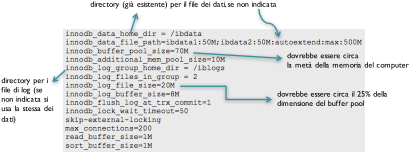
\includegraphics[scale=1]{figures/innoDB_settings.png}
\caption{InnoDB - Opzioni di configurazione} 
\end{figure}
\end{center}

Se nulla viene specificato di default MySQL crea nella directory dei dati:

\begin{itemize}

\item Un file dati di 10MB;
\item Due file di log da 5MB.

\end{itemize}

\subsubsection{InnoDB - Le Transazioni}

\begin{itemize}

\item Una transazione è una sequenza di operazioni sul DB cui si vogliono associare particolari caratteristiche di correttezza, robustezza, isolamento (es. bonifico bancario, acquisto biglietto, prenotazione aerea, ...);
\item Ogni connessione a MySQL inizia in autocommit mode e cioè tutte le istruzioni di aggiornamento vengono rese effettive immediatamente;
\item Disattivando l’autocommit con \textit{SET AUTOCOMMIT = 0}:

\begin{itemize}

\item Le modifiche diventeranno operative solo all’esecuzione dell’istruzione\newline \textit{COMMIT} (conferma l’operazione);
\item Eseguendo una \textit{ROLLBACK} invece (aborto operazione), verranno annullate tutte le modifiche fatte fino alla \textit{COMMIT} precedente;
\end{itemize}

\item Invece di disattivare l’autocommit, si possono utilizzare le transazioni iniziandole con \textit{START TRANSACTION} o \textit{BEGIN} e terminandole con \textit{COMMIT} o \textit{ROLLBACK}.

\end{itemize}

\subsubsection{InnoDB - le chiavi esterne}

\begin{itemize}

\item È possibile definire le foreign key, cioè collegare i valori delle colonne che contengono chiavi di altre tabelle alle tabelle stesse;
\item In questo modo è possibile verificare automaticamente quando i valori della tabella madre vengono modificati o eliminati in modo da:

\begin{itemize}

\item impedire queste modifiche;
\item o modificare di conseguenza anche i valori sulla tabella figlia
\end{itemize}

\end{itemize}

\begin{center}
\begin{figure}[H]
\centering
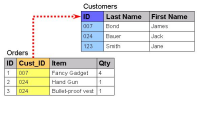
\includegraphics[scale=1]{figures/innoDB_fk.png}
\caption{InnoDB - Foreign Keys} 
\end{figure}
\end{center}

\begin{center}
\begin{figure}[H]
\centering
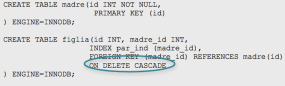
\includegraphics[scale=1]{figures/innoDB_fk_code.png}
\caption{InnoDB - Foreign Keys - Codice} 
\end{figure}
\end{center}

\begin{itemize}

\item Definizione di due tabelle (madre e figlia);
\item La figlia ha una chiave esterna sulla tabella madre;
\item Quando viene cancellata una riga dalla tabella madre, se il valore di id è presente in un campo madre\_id della tabella figlia, la riga corrispondente verrà eliminata.

\end{itemize}



ON DELETE / ON UPDATE:

\begin{itemize}
\item{\textbf{CASCADE}}: la cancellazione o modifica di un record nella tabella madre genererà la cancellazione o la modifica dei record collegati nella tabella figlia;
\item{\textbf{SET NULL}}: in caso di eliminazione o modifica di un record nella tabella madre i record collegati della tabella figlia verranno modificati impostando il campo NULL (opzione attivabile solo se il campo interessato della tabella figlia non è impostato a NOT NULL);
\item{\textbf{SET DEFAULT}}: in caso di eliminazione o modifica di un record nella tabella madre i record collegati della tabella figlia verranno impostati al valore di default;
\item{\textbf{RESTRICT}}: non permette cancellazioni sulla tabella madre se ci sono valori presenti nella tabella figlia;
\item{\textbf{NO ACTION}}: non permette cancellazioni sulla tabella madre se ci sono valori presenti nella tabella figlia.

\end{itemize}

Le opzioni NO ACTION e RESTRICT sono tra loro molto simili: in entrambi i casi, se la verifica del vincolo fallisce, l'operazione porta ad un errore.

La principale differenza tra le due è che con l'opzione NO ACTION, la verifica del vincolo di integrità è fatta \textit{dopo} aver tentato di modificare la tabella esterna, mentre con l'opzione RESTRICT la verifica è fatta \textbf{prima} di tentare l'esecuzione del DELETE.


\subsection{AUTO-INCREMENT}

\begin{itemize}

\item MyISAM gestisce una colonna di tipo auto-increment per ogni tabella:

\begin{itemize}

\item incrementa automaticamente il suo valore per ogni riga scritta;
\item i valori eliminati non vengono riutilizzati nemmeno se sono gli ultimi della sequenza;

\end{itemize}

\item InnoDB gestisce il valore auto-increment in modo particolare:

\begin{itemize}

\item calcola il valore la prima volta che si rende necessario dopo l’avvio del server selezionando il valore massimo esistente sulla tabella e incrementandolo di 1;
\item il valore viene conservato in memoria ma non scritto sul disco per cui al riavvio successivo sarà ricalcolato $\rightarrow$ se fossero cancellati ad esempio gli ultimi valori della tabella e non venissero effettuati nuovi inserimenti, al successivo riavvio il server utilizzerà quei valori.

\end{itemize}

\end{itemize}

Quale motore utilizzare? DIPENDE! 

\begin{itemize}

\item{InnoDB}: ideale per applicazioni dove il data integrity è importante e dove ci sono molteplici inserimenti e update;
\item{MyISAM} è veloce e ideale per applicazioni dove vengono effettuate molteplici select e poco dipendenti dal data integrity.

\end{itemize}

Qual'è il motore di default? 

\begin{itemize}

\item Comando SQL:

\begin{lstlisting}[language=SQL]
SHOW ENGINES
\end{lstlisting}

\item File di configurazione \textit{my.ini}:

\begin{lstlisting}[language=Ini]
default-storage-engine = MyISAM # o InnoDB
\end{lstlisting}

Che può essere usato anche per impostare il default storage engine
(oppure default-table-type)

\item Alla creazione della tabella:

\begin{itemize}
\item
\begin{lstlisting}[language=SQL]
CREATE TABLE tabella (a INT) ENGINE = INNODB;
\end{lstlisting}
\end{itemize}

\item Modifica del motore:

\begin{itemize}
\item
\begin{lstlisting}[language=SQL]
ALTER TABLE tabella ENGINE = INNODB;
\end{lstlisting}
\end{itemize}
\end{itemize}

\subsection{Tipi di dato in SQL}

\begin{itemize}

\item Tipo numerico:

\begin{center}
\begin{figure}[H]
\centering
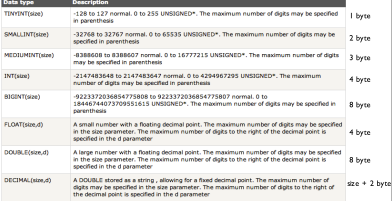
\includegraphics[scale=1]{figures/mySQL_numeric.png}
\caption{MySQL - Tipo di dato Numerico} 
\end{figure}
\end{center}

\item Tipo alfanumerico:

\begin{center}
\begin{figure}[H]
\centering
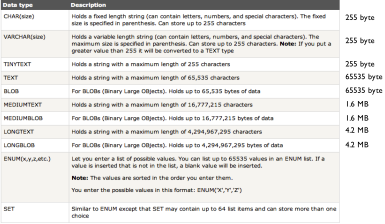
\includegraphics[scale=1]{figures/mySQL_alphanumeric.png}
\caption{MySQL - Tipo di dato Alfanumerico} 
\end{figure}
\end{center}

\item Tipo temporale:

\begin{center}
\begin{figure}[H]
\centering
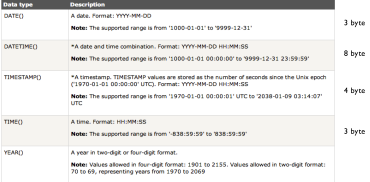
\includegraphics[scale=1]{figures/mySQL_time.png}
\caption{MySQL - Tipo di dato Temporale} 
\end{figure}
\end{center}

\begin{itemize}

\item Esiste pochissima coerenza nelle funzioni di data e ora tra i diversi produttori di DBMS;
\item In gran parte questo dipende dal fatto che molti produttori hanno sviluppato i tipi di dati per data e ora prima dello sviluppo degli standard.

\end{itemize}

\end{itemize}

Funzioni data/ora:

\begin{itemize}

\item{SQL Server}:

\begin{center}
\begin{figure}[H]
\centering
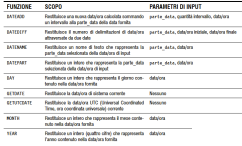
\includegraphics[scale=1]{figures/SQLserver_time.png}
\caption{SQL Server - Funzioni data/ora} 
\end{figure}
\end{center}

\item{Oracle}:

\begin{center}
\begin{figure}[H]
\centering
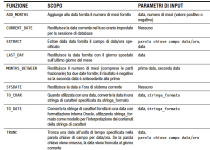
\includegraphics[scale=1]{figures/oracle_time.png}
\caption{Oracle DB - Funzioni data/ora} 
\end{figure}
\end{center}

\item{MySQL} dispone di oltre 30 funzioni di data e ora. Le più utilizzate:

\begin{center}
\begin{figure}[H]
\centering
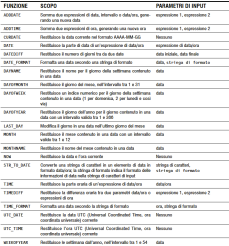
\includegraphics[scale=1]{figures/mySQL_data_ora.png}
\caption{MySQL - Funzioni data/ora} 
\end{figure}
\end{center}

\end{itemize}

\begin{itemize}

\item Le seguenti funzioni mostrano a video la data e l’ora attuale:

\begin{lstlisting}[language=SQL]
SELECT CURDATE()
SELECT CURTIME()
SELECT NOW()
\end{lstlisting}

che ritornano rispettivamente:

\begin{itemize}

\item 2013-10-02 (aaaa/mm/gg);
\item 13:02:57 (hh:mm:ss);
\item 2013-10-02 13:02:57 (aaaa/mm/gg hh:mm:ss).

\end{itemize}

\end{itemize}

Formattazione delle date:

\begin{center}
\begin{figure}[H]
\centering
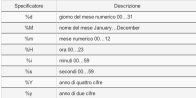
\includegraphics[scale=1]{figures/mySQL_dateformat.png}
\caption{MySQL - Formato date} 
\end{figure}
\end{center}

\begin{center}
\begin{figure}[H]
\centering
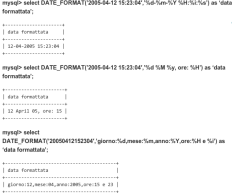
\includegraphics[scale=1]{figures/mySQL_dateformat2.png}
\caption{MySQL - Formato date} 
\end{figure}
\end{center}

Per la formattazione del tempo si può usare la funzione \textbf{TIME\_FORMAT()}, del tutto analoga a DATE\_FORMAT, ma che utilizza solo gli specificatori di formato che manipolano ore, minuti e secondi. 

\begin{itemize}

\item Dalla versione 4.1.1 di MySQL è disponibile la funzione \textbf{STR\_TO\_DATE()}, inversa di DATE\_FORMAT;
\item Essa riceve come argomenti la stringa contenente la data e la corrispondente stringa di formattazione e restituisce un valore DATETIME, DATE o TIME a seconda delle circostanze.

\end{itemize}

\begin{center}
\begin{figure}[H]
\centering
\includegraphics[scale=1]{figures/mySQL_strtodate.png}
\caption{MySQL - Funzione STR\_TO\_DATE()} 
\end{figure}
\end{center}

Timestamp:

\begin{itemize}

\item Campo utile per determinare automaticamente l’istante in cui un certo record è stato inserito o modificato;
\item\textbf{Nota}: se la tabella contiene più campi TIMESTAMP solo il primo sarà automaticamente aggiornato (dalla versione 4.1.2 di MySQL si può specificare quale colonna aggiornare).
\item Per ottenere tale automatismo sarà sufficiente non specificare nelle istruzioni di INSERT o UPDATE il valore per la colonna in oggetto oppure impostarla a NULL;
\item Il formato di visualizzazione del TIMESTAMP varia a seconda del valore specificato per “dimensione”;
\item Es. considerando la data del 20 maggio 2005 19:11:02.

\end{itemize}

\begin{center}
\begin{figure}[H]
\centering
\includegraphics[scale=1]{figures/mySQL_timestamp.png}
\caption{MySQL - TIMESTAMP()} 
\end{figure}
\end{center}

Funzioni per la somma e la sottrazione del tempo:

\begin{center}
\begin{figure}[H]
\centering
\includegraphics[scale=1]{figures/mySQL_addsubdate.png}
\caption{MySQL - Somma e Sottrazione temporale} 
\end{figure}
\end{center}

\begin{itemize}

\item Sommare 10 giorni alla data corrente:

\begin{lstlisting}[language=SQL]
SELECT DATE_ADD(CURDATE(),INTERVAL 10 DAYS);
\end{lstlisting}

\item Sottrarre 2 mesi da una data specifica:

\begin{lstlisting}[language=SQL]
SELECT DATE_SUB('2005-01-23',INTERVAL 2 MONTHS);
\end{lstlisting}
\item Aggiungere 7 mesi al mese di gennaio 2005:

\begin{lstlisting}[language=SQL]
SELECT PERIOD_ADD(200501,7);
\end{lstlisting}
\item Sottrarre 3 mesi al mese di gennaio 2005:
\begin{lstlisting}[language=SQL]
SELECT PERIOD_ADD(200501,-3);
\end{lstlisting}
\item Trovare la differenza (espressa in mesi) tra il gennaio 2005 ed ottobre 2002:
\begin{lstlisting}[language=SQL]
SELECT PERIOD_SUB(200501,200210);
\end{lstlisting}
\end{itemize}


\subsection{Funzioni di aggregazione}

\begin{itemize}

\item Le funzioni di aggregazione non lavorano su un solo dato ma su insiemi di dati $\rightarrow$ restituiscono un unico valore come “sintesi” di n valori;
\item Le funzioni principali:
\begin{itemize}

\item COUNT restituisce un intero che indica il numero di record trovati;
\item AVG restituisce la media;
\item MIN e MAX restituiscono il minore e il maggiore rispettivamente;
\item SUM restituisce la somma tra più record dello stesso campo.

\end{itemize}

\begin{center}
\begin{figure}[H]
\centering
\includegraphics[scale=1]{figures/mySQL_aggregation.png}
\caption{MySQL - Fuzioni di aggregazione} 
\end{figure}
\end{center}
\item Nell'utilizzo di una funzione di aggregazione è importante (consigliato, anche se non obbligatorio) specificare un alias per il risultato, con l'utilizzo della clausola \textbf{AS}.

\item Le funzioni di aggregazione vengono usate spesso in combinazione con la clausola \textbf{GROUP BY} $\rightarrow$ funzioni svolte non su tutte le righe estratte dalla WHERE, ma singolarmente su ogni gruppo di righe formato dalla GROUP BY;
\item Lo standard SQL vuole che in una SELECT che contiene funzioni di aggregazione tutte le colonne su cui tali funzioni non lavorano siano comprese nella GROUP BY;
\item Es. questa query non sarebbe valida: manca la GROUP BY sul campo nome:

\begin{center}
\begin{figure}[H]
\centering
\includegraphics[scale=1]{figures/mySQL_invalidquery.png}
\caption{MySQL - Query invalida per via della mancanza del campo nome in GROUP BY} 
\end{figure}
\end{center}

\item La query ha tuttavia un senso logico, perché il valore di nome, dipendendo dalla join, sarà sempre lo stesso in ogni gruppo di righe con lo stesso ‘idCliente’: di conseguenza è superfluo inserirlo nella GROUP BY;
\item MySQL quindi ci consente di usare questa sintassi: bisogna però fare attenzione a non mettere la GROUP BY su un campo che non ha un valore unico, in quanto ne otterremmo un risultato non prevedibile.

\end{itemize}

\begin{itemize}

\item{\textit{COUNT}}:

\begin{itemize}

\item Viene utilizzata per recuperare il numero di righe di una colonna;
\item Può essere utilizzata su qualunque tipo di dato.

\begin{center}
\begin{figure}[H]
\centering
\includegraphics[scale=1]{figures/mySQL_count.png}
\caption{MySQL - Funzione COUNT} 
\end{figure}
\end{center}

\textbf{Variante: COUNT(DISTINCT)};
\item Restituisce il numero delle diverse combinazioni che non contengono il valore NULL;
\item Es. in una colonna abbiamo 10 righe: 5 contenenti la parola "calcio", 3 contenenti "tennis" e le ultime 2 con "golf”. Effettuando un COUNT(DISTINCT) avremo il numero di combinazioni diverse, ovvero 3 (calcio, tennis, golf).

\begin{lstlisting}[language=SQL] 
SELECT COUNT(DISTINCT nomeCampo) FROM nomeTabella; 
\end{lstlisting}
\end{itemize}


\item{\textit{MAX/MIN}}:

\begin{itemize}

\item{\textbf{MAX}}: restituisce il valore più alto contenuto all'interno di una colonna;
\item Per i campi numerici, restituisce il numero più alto, per quelli testuali (nei nuovi MySQL questa operazione è permessa) seleziona il campo che secondo l'ordine alfabetico è più avanti:

\begin{lstlisting}[language=SQL]
SELECT MAX(nomeCampo) FROM nomeTabella;
\end{lstlisting}

\item{\textbf{MIN}}: fa esattamente l'opposto della precedente: prende il valore più basso:

\begin{lstlisting}[language=SQL]
SELECT MIN(nomeCampo) FROM nomeTabella;
\end{lstlisting}
\end{itemize}

\begin{center}
\begin{figure}[H]
\centering
\includegraphics[scale=1]{figures/mySQL_maxmin.png}
\caption{MySQL - MIN/MAX} 
\end{figure}
\end{center}


\item{\textit{AVG/SUM}}:

\begin{itemize}

\item{\textbf{AVG}}: restituisce una media dei valori presenti in un campo (va applicata ai soli campi numerici):

\begin{center}
\begin{figure}[H]
\centering
\includegraphics[scale=1]{figures/mySQL_avg.png}
\caption{MySQL - Funzione AVG} 
\end{figure}
\end{center}

\item{\textbf{SUM}}: somma i valori contenuti nel campo (va applicata ai soli campi numerici);

\begin{center}
\begin{figure}[H]
\centering
\includegraphics[scale=1]{figures/mySQL_sum.png}
\caption{MySQL - Funzione SUM} 
\end{figure}
\end{center}

\end{itemize}


\item{\textit{GROUP BY}}:

\begin{center}
\begin{figure}[H]
\centering
\includegraphics[scale=1]{figures/mySQL_groupby.png}
\caption{MySQL - Clausola GROUP BY} 
\end{figure}
\end{center}

\begin{center}
\begin{figure}[H]
\centering
\includegraphics[scale=1]{figures/mySQL_groupby2.png}
\caption{MySQL - Clausola GROUP BY 2} 
\end{figure}
\end{center}


\item{\textit{HAVING}}:

\begin{itemize}

\item Usando la clausola GROUP BY, generalmente non si è interessati a tutti i risultati della selezione, ma solo ad alcuni gruppi che possiedono determinati requisiti:

\begin{center}
\begin{figure}[H]
\centering
\includegraphics[scale=1]{figures/mySQL_having.png}
\caption{MySQL - Clausola WHERE} 
\end{figure}
\end{center}

\item WHERE identifica un set iniziale di record che poi vengono selezionati dalla tabella:

\begin{center}
\begin{figure}[H]
\centering
\includegraphics[scale=1]{figures/mySQL_having2.png}
\caption{MySQL - Clausola WHERE + GROUP BY} 
\end{figure}
\end{center}

\item Aggiungendo alla query la clausola GROUP BY e qualche funzione di aggregazione, i record vengono raggruppati e per ogni gruppo vengono eseguiti i calcoli richiesti;

\item Aggiungendo una clausola HAVING, viene ristretto il numero di record mostrati:

\begin{center}
\begin{figure}[H]
\centering
\includegraphics[scale=1]{figures/mySQL_having3.png}
\caption{MySQL - Clausola HAVING} 
\end{figure}
\end{center}

\item WHERE: riduce il numero di record da processare fin dall’inizio e quindi rende la query più efficiente;
\item Scegliere i valori da mostrare usando HAVING senza prima aver limitato i record da processare con WHERE, può rendere la query più pesante, perché verrebbero eseguiti raggruppamenti e calcoli effettuati dalle funzioni di aggregazione su record che non interessano;

\end{itemize}

\end{itemize}


\subsection{phpMyAdmin – indici}

\begin{itemize}

\item In MySQL è possibile creare diversi tipi di indice:

\begin{center}
\begin{figure}[H]
\centering
\includegraphics[scale=1]{figures/mySQL_index.png}
\caption{MySQL - Tipi di indici} 
\end{figure}
\end{center}

\item{\textbf{Primary Key}}: indice associato alla chiave primaria, non può contenere valori NULL né valori duplicati. Usato spesso in associazione con la direttiva auto\_increment in caso di valori numerici unici;
\item{\textbf{Index}} utilizzato per velocizzare l'accesso ai dati. A differenza della chiave primaria l’indice non è unico e può essere creato per accelerare l'elaborazione delle query. Ci possono essere valori duplicati e valori NULL;
\item{\textbf{Unique}} come index, solo che tutti i valori del campo indicizzato univoco devono comparire solo una volta (non ci possono essere valori duplicati), sono consentiti valori NULL;
\item{\textbf{Fulltext}} indice specializzato per la ricerca di parole nei testi. È supportato per i campi di tipo VARCHAR e TEXT.

\end{itemize}


\subsection{Popolare database}

\begin{itemize}

\item Supponiamo di avere un’entità Person e di volerla popolare con tanti dati random ma \textbf{validi} in base al tipo di attributo considerato:

\begin{center}
\begin{figure}[H]
\centering
\includegraphics[scale=1]{figures/person_entity_pop.png}
\caption{Entità Person} 
\end{figure}
\end{center}

\item Sul web esistono diverse sorgenti dati utili ai fini del popolamento di database per poter eseguire querye fare test;
\item Supponiamo di voler utilizzare Excel “come appoggio”

\end{itemize}

Considerando la nostra entità ci occorre:

\begin{itemize}

\item Elenco di nomi \url{https://gist.github.com/pdesterlich/2562329};
\item Elenco di cognomi \url{https://gist.github.com/pdesterlich/2562407};
\item Elenco delle regioni italiane (piccolo elenco: copia e incolla dal web; ma anche con sql \url{https://gist.github.com/TheHiddenHaku/7103443});
\item Elenco delle province italiane \newline\url{https://gist.github.com/iamlucamilan/0727b08c2ab9a4e83cc3};
\item Elenco province e regioni \newline\url{http://www.mandile.it/wp-content/uploads/provinciaregione-sigla.csv};
\item Elenco città italiane con CAP \url{http://lab.comuni-italiani.it/download/comuni.html};
\item Per gli altri attributi (es. civico) usiamo funzioni di Excel $=CASUALE.TRA(1; 50)$

\end{itemize}

Per la generazione di dati random è necessario scrivere qualche funzione VBA (\textbf{Visual Basic Editor}):

\begin{itemize}

\item{\underline{Windows}}: Alt + F11;
\item{\underline{MAC Os}}: Fn + Alt + F11 oppure menu Strumenti $\rightarrow$ Macro $\rightarrow$ Visual Basic Editor.

\end{itemize}

\begin{lstlisting}[language={[Visual]Basic}]
Function random_name()
	a = Rnd()
	b = range("a50").Value
	x = 50 + Int(a * b)
	r = range("B" & CStr(x))
	random_name = r
End Function
\end{lstlisting}

La funzione \textbf{Rnd()} restituisce un numero reale fra 0 e 1 (estremi esclusi) In generale, come trasformare il numero casuale in un numero intero compreso fra min e max? \textbf{Int(Rnd()*(max-min+1))+min}.

Per generare date di nascita random: 

\begin{lstlisting}[language={[Visual]Basic}]
Function random_date_between(x, y) As Date
	a = Rnd()
	b = DateDiff("d", x, y)
	r = CDate(x) + CDate(Int(a * b))
	random_date_between = r
End Function
\end{lstlisting}


\begin{center}
\begin{figure}[H]
\centering
\includegraphics[scale=1]{figures/excel_populated2.png}
\caption{Microsoft Excel - Popolamento completato} 
\end{figure}
\end{center}

Una volta ottenuta la sorgente dati, si può salvare il file in formato csv per poi importarlo sul DB.


\begin{flushright}Lucia Vaira\\27/10/2016\end{flushright}


\section{SQL Recap}

SQL non è un vero linguaggio di programmazione perché ogni cosa può essere rappresentata come una singola espressione. Anche operazioni molto complesse possono essere ricondotte essenzialmente a un’unica espressione. Questo linguaggio si fonda quindi su un paradigma dichiarativo,  come avviene in linguaggi come HTML, in cui abbiamo vari tag che specificano ciò che deve essere visualizzato sullo schermo. In SQL dobbiamo dire ciò di cui abbiamo bisogno, non come fare per ottenerlo. Eventuali ottimizzazioni delle query e le decisioni su come eseguirle sono prese in carico dal DBMS. Abbiamo solo insiemi e operatori che ci permettono di combinare tali insiemi. \textbf{Regola Fondamentale: Non scrivete algoritmi basati su SQL}. La gestione dei dati si fa in SQL.  Non usate Java per il data layer. Java, piuttosto che C++ o PHP, va bene per il presentation layer, e in parte per la business logic, ma i dati deve gestirli il DBMS. Tranne casi rarissimi, non si scrivono algoritmi di manipolazione dati per la gestione dei database.   

SQL sta per Structured Query Language. Ultimo standard è  SQL99. Se vi sembra obsoleto, sappiate che dentro ci sono cose così avanzate che ancora devono essere implementate tutte. La base però sta in ciò che abbiamo detto per l’algebra relazionale. Per comprendere meglio cosa è SQL,  dobbiamo avere chiaro in mente il ciclo di vita dei database e il ciclo di vita dei dati. Un database è una collezione di dati e vincoli. Quando progettiamo un database lo traduciamo in tabelle e vincoli e poi lo spostiamo su una macchina fisica.  Le operazioni che si possono fare sono:  

\textbf{Schema creation}: il primo comando che impariamo è CREATE SCHEMA. Nello schema possiamo creare tabelle, con dei vincoli, delle viste (tabelle virtuali ottenute da tabelle reali attraverso operatori, come quando facciamo una join). Possiamo creare funzioni, modificarle ecc… Infine abbiamo \textit{stored procedures} (create in un linguaggio presente nel DBMS). Sono programmi in grado di estrarre informazioni dalle tabelle, scritti in un linguaggio specifico. Tali funzioni vivono nel DBMS. Possiamo anche utilizzare linguaggi esterni tramite appositi plugin. È importante dire che oltre ai database che creiamo noi per memorizzare informazioni, esiste anche un meta-database, o \textbf{catalogo}, presente nel DBMS, che si può pensare come la collezione di tutti gli schemi che abbiamo creato, con i relativi oggetti, tabelle, funzioni, viste, ecc. Mysql è basato su un catalogo di sistema, che è un database, contenente informazioni sugli altri database. Ci sarà il tipo di entità  'entità ', un altro 'vincoli di chiave esterna', ecc… Quando vogliamo informazioni sul database,  interroghiamo il system catalog.  

CREATE SCHEMA crea una cartella vuota in cui mettiamo tutte le nostre tabelle. Ogni schema corrisponde a un database separato. Non andiamo a mischiare informazioni non appartenenti allo specifico database. Normalmente le tabelle usano la notazione puntata. Ad esempio se vogliamo la tabella ‘persona’ dallo schema ‘amici’, scriviamo SELECT from amici.persona.  

I DBMS non solo hanno tabelle, ma sono in grado di gestire utenti e gruppi,  ciascuno col suo set di autorizzazioni. Se ad esempio scriviamo:

\begin{lstlisting}[language=SQL]
CREATE SCHEMA COMPANY AUTHORIZATION 'Jsmith'
\end{lstlisting}

allora Jsmith sarà il proprietario dello schema creato e avrà privilegi esclusivi di accesso e modifica. Se non si specifica l’autorizzazione, tipicamente l’owner del database è autorizzato a far tutto.   
Quando lo schema è pronto, possiamo creare e modificare le tabelle. CREATE TABLE COMPANY.EMPLOYEE crea la tabella EMPLOYEE nel database COMPANY.  Quando le tabelle sono create, allora operiamo con un set differente di comandi. Inizia il ciclo di vita dei dati. Abbiamo a disposizione differenti tipi di dati:

\begin{itemize}

\item{Numerici}: SMALLINT corrisponde a 1 o 2 byte, int 2 o 4 byte, LONGINT fino a 8 byte. Quando facciamo funzioni di aggregazione possiamo ottenere overflow se non dimensioniamo bene i tipi di dato. Si specifica anche la cifra di precisione. Vi sono poi i numeri in virgola mobile,  tipo FLOAT o REAL o DOUBLE. Nel passaggio di dati da una macchina all'altra bisogna stare attenti alla compatibilità delle due macchine;
\item{Stringhe}: I gigabyte costano niente per cui è abbastanza facile avere memoria. Un singolo byte può fare la differenza quando è moltiplicato per milioni di volte. VARCHAR (1000) vuol dire che se mettiamo un nome di 10 lettere, non consumiamo 1000, perché VARCHAR si adatta alle dimensioni. Ma è anche time-consuming. Se il database deve essere veloce usiamo CHARACTER. Con CLOB ogni cella può memorizzare miliardi di caratteri. È utile per grandi documenti tipo pdf;
\item{Bit string}: usate essenzialmente per dati provenienti da apparecchiature.
\item{Boolean}: TRUE o FALSE;
\item{DATE}: la data ha dieci posizioni distinte. Timestamp contiene la data e ora completa e consente anche di specificare la time zone.  

\end{itemize}

Esiste anche un meccanismo di estensione CREATE DOMAIN, che è solo un modo diverso di assegnare valori predefiniti a certi tipi di dato,  come si fa con typedef in C. 

\subsection{VINCOLI}


\begin{itemize}

\item{\textbf{Default value}}: valore che assume il dato se non viene specificato;

\item Un vincolo interessante è il \textbf{CHECK}: quando inseriamo un dato viene sempre verificato che sia rispettato quel check. Ad esempio, tutte le volte che si inserisce un nuovo dipendente, verifica che abbia più di 18 anni, altrimenti non lo assumi.  Tale controllo può essere esteso tramite i trigger, che agiscono sull’intera tabella, ad esempio si può dire ‘non inserire questo dipendente se l'età media supera un certo valore’;

\item{\textbf{Integrità referenziale}}:

Prima di tutto, posso dire che un certo attributo è unico; il concetto di unicità  è associato alla chiave primaria. Si può anche introdurre una chiave secondaria che sia unica. Per quanto riguarda le chiavi esterne, si possono specificare vari tipi di azioni: ON UPDATE CASCADE, SET DEFAULT, SET NULL. Se cancello una merce, cancella tutte le vendite. Questo è il \textbf{cascade}. Potrei anche dire on delete set null, oppure set default, ovvero tutte le volte che cancello un cliente, assegna le vendite a un cliente generico. Si tratta di operazioni fatte in automatico quando si cancella o modifica un dato con vincoli di integrità referenziale.  

\end{itemize}
 
I vincoli possono essere messi alla fine di ogni tabella. Oppure posso dargli un nome in modo che posso richiamarlo in un ALTER CONSTRAINT per modificarlo in seguito. È buona norma dare un nome per evitare di riscrivere tutto. 

\subsection{Meccanismo base Query}

Il meccanismo di base delle query è basato sul costrutto: 

\begin{lstlisting}[language=SQL]
SELECT <attribute list>
FROM <table list>
WHERE <condition> 
\end{lstlisting}

Ad esempio,

\begin{lstlisting}[language=SQL]
SELECT Fname, Lname, Address
FROM EMPLOYEE, DEPARTMENT
WHERE Dname = 'Research' AND Dnumber = Dno; 
\end{lstlisting}

Restituisce nome e indirizzo di tutti gli impiegati che lavorano nel dipartimento “Ricerca”. Si dice che Dname = ‘Research’ è una selection condition, mentre Dnumber = Dno è una join condition. Per evitare ambiguità con gli attributi, si può preporre un attributo con il nome della relazione, avvalendosi della notazione puntata. Per abbreviare, si può rinominare la relazione con un \textbf{alias}.
  
Infine, alle tabelle si possono applicare le normali funzioni insiemistiche come UNION o INTERSECT, con la possibilità di specificare se si vogliono elementi tutti distinti, o si permettono i duplicati.   


\subsection{ESERCIZIO}

Si vuole progettare una base di dati per la raccolta e la gestione di informazioni relative al contesto di una specifica stagione di Formula 1. A tale scopo sono stati ricavati i seguenti requisiti:

\begin{itemize}

\item Calendario Competizione;
\item Piloti;
\item Veicoli;
\item Classifica Piloti;
\item Classifica Marche;
\item Circuiti $\rightarrow$ Posti disponibili $\rightarrow$ Clienti;
\item Meteo;
\item Team  

\end{itemize}

Essendo il primo requisito equivoco sotto certi aspetti (accorpamento dei propri attributi in altri requisiti), si è passati alla trattazione del secondo, identificandolo come un’entità e ricavandone i relativi attributi. 

\begin{center}
\begin{figure}[H]
\centering
\includegraphics[scale=1]{figures/pilot_entity.png}
\caption{Entità PILOTA} 
\end{figure}
\end{center}

In seguito si è associata l’entità \textit{PILOTA} all’entità \textit{VEICOLO} (derivante dal requisito 3) tramite la relazione \textit{GUIDA}, contenente informazioni su data, ora e setup del veicolo, che sarà soggetto a variazioni durante lo svolgimento delle varie corse.   

\begin{center}
\begin{figure}[H]
\centering
\includegraphics[scale=0.8]{figures/pilota_guida_veicolo.png}
\caption{Relazione Pilota-Guida-Veicolo} 
\end{figure}
\end{center}

Dalla discussione dei requisiti successivi è emerso che:

\begin{itemize}

\item I requisiti Team, Corsa e Circuito sono stati identificati come entità;
\item Il requisito meteo è stato considerato attributo dell’entità \textit{CORSA};
\item Allo stesso modo il requisito Posti disponibili è stato trattato come attributo composto (Categoria + Numero) dell’entità \textit{CIRCUITO};
\item I requisiti sulla Classifica sono stati ritenuti calcolabili a partire dalle informazioni già contenute nel database;
\item Tra \textit{PILOTA} e \textit{CORSA} una doppia relazione (\textit{PARTECIPA} e \textit{SI QUALIFICA}), derivante dall’implementazione del pattern Preventivo-Consuntivo.   

\end{itemize}

\begin{center}
\begin{figure}[H]
\centering
\includegraphics[scale=0.8]{figures/formula1_incER.png}
\caption{Formula 1 - Incremental ER} 
\end{figure}
\end{center}

Ulteriori osservazioni hanno portato alla creazione di un’entità \textit{EVENTO} che tiene conto di accadimenti talvolta sporadici che possono coinvolgere piloti e veicoli in una corsa.   

\begin{center}
\begin{figure}[H]
\centering
\includegraphics[scale=0.8]{figures/formula1_incER2.png}
\caption{Formula 1 - Ultime modifiche} 
\end{figure}
\end{center}

Infine il requisito Cliente è stato identificato come entità e associato a \textit{CORSA} tramite il pattern Preventivo-Consuntivo. In conclusione si noti che la relazione tra CORSA e CIRCUITO è unaria in quanto ogni singola corsa si svolge su un singolo circuito, pervenendo alla seguente soluzione finale: 

\newpage
\begin{center}
\begin{figure}[H]
\centering
\includegraphics[scale=0.7]{figures/formula1_ER.png}
\caption{Formula 1 - ER finale} 
\end{figure}
\end{center}


\begin{flushright}Gioele Sforza\\Simone Dongiovanni\\02/11/2016\end{flushright}


\section{SQL per manipolare i dati}

In SQL esistono 3 comandi che possono essere usati per modificare i dati contenuti all’interno di una tabella: INSERT, DELETE, e UPDATE.

\begin{itemize}

\item{\textbf{Query di tipo INSERT}}

Nella sua forma più semplice, INSERT è usato per aggiungere una singola tupla (riga) in una relazione (tabella). È necessario specificare il nome della relazione e una lista di valori per la tupla. I valori devono essere specificati nello stesso ordine con cui sono stati specificati i relativi attributi nella query CREATE TABLE.

\begin{center}
\begin{figure}[H]
\centering
\includegraphics[scale=1]{figures/insert.png}
\caption{SQL INSERT} 
\end{figure}
\end{center}

Una seconda formulazione per INSERT consente di specificare esplicitamente gli attributi che corrispondono ai valori che si vogliono inserire:

\begin{center}
\begin{figure}[H]
\centering
\includegraphics[scale=1]{figures/insert2.png}
\caption{SQL INSERT con specifica esplicita degli attributi da inserire} 
\end{figure}
\end{center}

Gli attributi che non sono specificati in questa variante vengono settati al loro valore di default o a NULL. È importante che vengano sempre incluse le chiavi primarie e i campi che non possono assumere valore nullo. \textbf{ATTENZIONE}! Se si vuole modificare il valore contenuto all’interno di una riga, non si deve usare la INSERT specificando gli argomenti, ma bisogna usare una query di tipo UPDATE. Infatti, le INSERT creano sempre una nuova riga ogni volta che vengono eseguite.  

\item{\textbf{Query di tipo DELETE}}

Il comando DELETE rimuove tuple da una relazione. Specificando la condizione WHERE (che funziona come nelle query SELECT) è possibile selezionare quali tuple eliminare. Se invece non viene specificata, la DELETE procederà alla cancellazione di tutte le tuple contenute all’interno della relazione. 

\begin{center}
\begin{figure}[H]
\centering
\includegraphics[scale=1]{figures/delete.png}
\caption{SQL DELETE} 
\end{figure}
\end{center}

Spiegazione delle 4 queries:

\begin{itemize}

\item{U4A}: Elimina dalla relazione EMPLOYEE le tuple aventi l’attributo Lname impostato a ‘Brown’;
\item{U4B}: Elimina dalla relazione EMPLOYEE le tuple aventi l’attributo Ssn impostato a ‘123456789’;
\item{U4C}: Elimina dalla relazione EMPLOYEE le tuple aventi l’attributo Dno impostato a 5;
\item{U4D}: Elimina dalla relazione EMPLOYEE tutte le tuple.

\end{itemize}

Nonostante questo comando consenta di effettuare delle cancellazioni all’interno del database è importante notare che la legge italiana impone che i dati storici non debbano mai essere cancellati. Tali dati possono risultare importanti, ad esempio, per successive analisi statistiche di varia natura. In effetti, dato il basso costo che lo storage ha oggi, questo non rappresenta un problema. In ambito bancario, ad esempio, una persona potrebbe chiedere di essere cancellata: in tal caso, l’ente in questione è obbligato a farlo, conservando solo i dati rilevanti (come nome, cognome e il fatto che questa persona ha chiesto di essere cancellata). Ciò permette, in futuro, di non includere nuovamente questa persona all’interno di campagne promozionali. Gestire queste ed altre necessità è compito del responsabile dei dati (che è una figura necessaria quando le dimensioni del business sono importanti). Inoltre, è opportuno notare che quando si effettua una query DELETE, il DBMS adotta delle strategie che permettono di migliorare le performance. Infatti, le tuple eliminate dalla relazione non sono fisicamente rimosse dal filesystem, ma vengono solo rimosse dall’indice e lasciate sul disco. Questo produce un overhead della tabella che cresce man mano che si eliminano tuple dalla relazione. Solo successivamente è possibile ottimizzare la tabella usando alcuni comandi di amministrazione: nell’esecuzione di questi comandi, la tabella verrà distrutta e immediatamente ripopolata (eliminando dunque l’overhead su disco). È importante infine osservare che, generalmente, viene effettuato un backup dell’intero database ogni giorno (solitamente nelle ore notturne, quando non ci sono molti accessi al DB). Lo schema più usato prevede di effettuare un backup completo la domenica (poco traffico) e dei backup incrementali durante la settimana (molto traffico). Ciò significa che per ripristinare ad esempio il backup del mercoledì, sarà necessario applicare in sequenza i backup di domenica, lunedì, martedì, mercoledì. \textbf{File di log / journal }: tengono traccia di tutti gli I/O di un software. Nei database sono usati, tra l’altro, per ricostruire transazioni interrotte.  


\item{\textbf{Query di tipo UPDATE}}

Il comando UPDATE consente di modificare il valore degli attributi di una o più tuple selezionate. Come nel comando DELETE, anche qui è possibile inserire la clausola WHERE che permette di selezionare quali tuple modificare. \textbf{Nota bene}: Come nel caso della DELETE, non specificare la clausola WHERE equivale a modificare \textbf{tutte} le tuple di una tabella.   

\begin{center}
\begin{figure}[H]
\centering
\includegraphics[scale=1]{figures/update.png}
\caption{SQL UPDATE} 
\end{figure}
\end{center}

Spiegazione delle due query:

\begin{itemize}

\item{U5}: Modifica le tuple della relazione PROJECT aventi Pnumber pari a 10 impostando l’attributo Plocation a ‘Bellaire’ e l’attributo Dnum a 5;
\item{U6}: Modifica le tuple della relazione EMPLOYEE aventi Dno pari a 5 aumentando del 10\% l’attributo Salary.

\end{itemize}

\end{itemize}


\subsection{Transazioni e concorrenza (accenno)}

Due feature fondamentali dei database sono le \textbf{transazioni} e la \textbf{concorrenza}. Le accenniamo brevemente e le riprenderemo in seguito. Partiamo ad un breve esempio. Supponiamo che 10 utenti debbano effettuare un acquisto online di un dato prodotto e che siano disponibili solo 5 esemplari di quel prodotto. Supponiamo che solo 5 utenti su 10 abbiano la reale intenzione di acquistare il prodotto e che gli altri 5 decidano di rinunciare all’acquisto nella 
fase finale della procedura. Un classico problema posto da questo esempio che ricorre quando si modellano database per l’acquisto online è il seguente: come gestire il blocco del prodotto?  Se si opta per bloccare il prodotto una volta iniziata la procedura d’acquisto potrebbe accadere che i 5 utenti realmente interessati non possano acquistarlo a causa dei 5 utenti non interessati che rinunceranno al prodotto solo al termine della loro procedura. Questo arrecherebbe danno al venditore poiché 5 persone realmente intenzionate all’acquisto non trovano disponibilità per il prodotto, mentre altre 5 vi rinunciano all’ultimo momento, e la merce resterebbe invenduta.  Se si opta per bloccare il prodotto nell’ultima fase della procedura d’acquisto, la merce potrebbe essere stata acquistata da un altro utente pochi istanti prima di terminare l’acquisto e in tal caso non sarebbe possibile completare l’acquisto. Questo porterebbe l’utente a non essere soddisfatto del sito e quindi anche in questo caso ci sarebbe un danno per il venditore. In situazioni come questa la scelta migliore è quella di usare tecniche statistiche, con le quali si blocca ogni minuto il numero medio di prodotti acquistati al minuto. Se ad esempio un’attività vende un certo prodotto 5 volte al minuto, il software deciderà di bloccare ogni minuto una quantità pari a 5 per quel prodotto. Chiaramente, questo tipo di approccio è possibile solo nel caso in cui il business è sufficientemente grande da poter usare la statistica. Caratteristiche importanti che un database deve possedere sono riassunte nell’acronimo \textbf{ACID} (Atomicità, Consistenza, Isolamento e Durabilità). Per arrivare ad ottenere un database con queste caratteristiche si sfruttano tecniche matematiche. I database relazionali hanno il vantaggio di godere della proprietà ACID, e hanno quindi la caratteristica di non essere penetrabili. Tale pregio lo si paga in termini di scalabilità e velocità: usando architetture parallele e tracciando lo speedup in funzione dei processori, ad un certo punto la velocità di aumento dello speedup diventa sublineare. I database NoSQL (Not only SQL) non godono generalmente della proprietà ACID e sono invece più performanti su larga scala, ma accettano come ipotesi di perdere qualche informazione. Pertanto questi database perdono in coerenza. La bravura del progettista deve essere quella di conoscere tutte le soluzioni possibili e di adattarle in base alle necessità poste dal problema. In una applicazione bancaria, ad esempio, potrebbe essere un grosso errore quello di adottare una soluzione NoSQL.  


\subsection{Algebra a tre livelli}

Nell’ambito del linguaggio SQL è stato necessario ridefinire l’algebra booleana, che generalmente consta di 2 valori (vero e falso), rendendola a tre livelli (vero, falso, null). Sono stati attribuiti 12 possibili significati differenti a NULL, tre dei quali sono:

\begin{itemize}

\item{\textit{Valore sconosciuto}} (ad esempio quando non si conosce la data di nascita di una persona);
\item{\textit{Valore non applicabile}} (ad esempio un attributo LivelloLaurea è NULL per chi non è laureato);
\item{\textit{Valore non disponibile/trattenuto}} (ad esempio se una persona non vuole fornire il proprio indirizzo).

\end{itemize}

A causa della presenza del valore NULL, le operazioni booleane sono state estese in modo naturale come riassunto in figura:   

\begin{center}
\begin{figure}[H]
\centering
\includegraphics[scale=1]{figures/three_level_algebra.png}
\caption{Algebra a tre livelli} 
\end{figure}
\end{center}

Se in una query ci fosse la necessità di fare confronti contenenti NULL, non è possibile utilizzare le operazioni di confronto classiche come $\{=,\ <>,\ >,\ <,\ \geq,\ \leq\}$, ma si possono usare gli operatori \textbf{IS / IS NOT}, poiché l’uguaglianza tra NULL non esiste. Ad esempio, la query seguente seleziona i nomi degli impiegati senza supervisori: 

\begin{center}
\begin{figure}[H]
\centering
\includegraphics[scale=1]{figures/ISNULL.png}
\caption{Esempio di utilizzo della clausola IS in SQL} 
\end{figure}
\end{center}

\subsection{Query più complesse}

\begin{itemize}

\item{\textbf{Query annidate}}

Le \textbf{query annidate} sono delle query di tipo select-from-where all’interno di una \textbf{query esterna}. Le query annidate possono comparire in qualunque clausola si renda necessario inserirle: possono essere contenute nel blocco FROM, o in quello WHERE, o anche in quello SELECT. Nella seguente query introduciamo l’operatore di confronto \textbf{IN}, che confronta un valore v con un insieme e restituisce TRUE se v è contenuto nell’insieme. 

\begin{center}
\begin{figure}[H]
\centering
\includegraphics[scale=1]{figures/IN.png}
\caption{Query annidata con clausola IN} 
\end{figure}
\end{center}

La query Q4A seleziona i numeri di progetto (distinti) il cui manager o gli impiegati che ci lavorano hanno cognome Smith. Le due query annidate selezionano rispettivamente i numeri di progetto il cui manager ha cognome Smith e i numeri di progetto su cui lavorano impiegati aventi il cognome Smith. Successivamente, la query esterna mette insieme i risultati delle due query interne e restituisce solo i valori distinti (DISTINCT). Se una query annidata restituisce un singolo attributo e un singolo valore (cioè una tabella con una sola riga e una sola colonna), il risultato della query è uno \textbf{scalare}. In tal caso, è possibile usare l’operatore = per il confronto. In generale, il risultato di una query annidata è una \textbf{tabella} (una relazione con in generale più di una riga e più di una colonna). SQL permette di usare dei confronti tra \textbf{tuple} di valori, mettendole tra parentesi. I confronti tra tuple funzionano come i confronti tra vettori. Due tuple si considerano uguali se e solo se tutti gli elementi corrispondenti delle due tuple sono uguali (ad esempio $[1,2,3] = [1,2,3]$). Due tuple si considerano diverse se e solo se c’è almeno un elemento corrispondente tra le due tuple che è diverso (ad esempio $[1,2,3] <> [1,1,3]$). 

\begin{center}
\begin{figure}[H]
\centering
\includegraphics[scale=1]{figures/IN2.png}
\caption{Query annidata} 
\end{figure}
\end{center}

La query riportata sopra seleziona gli Essn degli impiegati che lavorano allo stesso progetto e per lo stesso numero di ore dell’impiegato con Essn 123456789. È opportuno notare che quando si vogliono fare i confronti tra tuple è necessario che la tuple da confrontare abbiano lo stesso numero di elementi (ovvero che il numero di elementi tra parentesi a sinistra dell’operatore IN coincida col numero di attributi indicati nella SELECT della query annidata). 
Ci sono altri operatori che si possono usare per confrontare un valore v con un insieme (che è il caso delle query annidate). Query operatori sono ANY, SOME, ALL (SOME è sinonimo di ANY) e si applicano insieme ad un operatore di confronto come quelli visti finora $\{=,\ \leq,\ <,\ >,\ \geq\}$. Ad esempio, = ANY (o = SOME) verifica che l’elemento v sia uguale \textbf{ad almeno un elemento} dell’insieme (e quindi è equivalente a IN). Invece, $> ANY$ verifica che l’elemento v sia maggiore di almeno un elemento dell’insieme. Invece, $> ALL$ verifica che l’elemento v sia maggiore \textbf{di tutti gli elementi} dell’insieme. La seguente query restituisce il nome degli impiegati con salario maggiore di tutti gli impiegati del dipartimento 5: 

\begin{center}
\begin{figure}[H]
\centering
\includegraphics[scale=1]{figures/INALL.png}
\caption{Query annidata con clausola ALL} 
\end{figure}
\end{center}

\item{\textbf{Query annidate correlate}}


È possibile che una query annidata contenga un riferimento ad un attributo gestito dalla query esterna. In questo caso si dice che le due query sono \textbf{correlate}:

\begin{itemize}

\item Le query annidate standard vengono valutate una volta. Il risultato è usato poi dalla query esterna;
\item Le query annidate correlate vengono valutate una volta per ogni tupla (o combinazione di tuple) nella query esterna. Ad esempio, se voglio trovare le persone che guadagnano più dei loro parenti, non posso calcolare l’insieme dei parenti una volta per tutte, ma devo rifarlo per ogni persona.  

\end{itemize}

Questa query restituisce i nomi degli impiegati che hanno dei dipendenti con il loro stesso nome e sesso: 

\begin{center}
\begin{figure}[H]
\centering
\includegraphics[scale=1]{figures/complexIN.png}
\caption{Query annidata correlata} 
\end{figure}
\end{center}

Spiegazione: Per ogni tupla di EMPLOYEE, viene valutata la query interna, che trova il Ssn dei dipendenti con il loro stesso nome e sesso. Successivamente, per ognuno di questi Ssn viene restituito il nome e il cognome. Il ragionamento viene ripetuto su ogni tupla di EMPLOYEE. È importante quando ci sono query annidate correlate che non ci sia ambiguità negli attributi, cioè non ci possono essere attributi aventi lo stesso nome nella query interna e in quella esterna. Per risolvere queste situazioni, si rende necessario l’uso degli alias come già visto in precedenza per identificare univocamente ogni oggetto presente nella query. Per quanto riguarda le prestazioni, è immediato comprendere che nel caso di query annidate correlate le performance si degradano molto più velocemente che nelle query annidate standard. Infatti, nelle query annidate standard il tempo di esecuzione è lineare nella dimensione della tabella, mentre nelle query annidate correlate il tempo di esecuzione è quadratico nella dimensione della tabella. Fortunatamente, molte delle query annidate correlate sono riscrivibili come una query non annidata con dei JOIN. Il DBMS ha un ottimizzatore incorporato che provvede ad effettuare questa operazione ogni volta che è possibile (riportando la complessità da quadratica a lineare).  


\item{\textbf{Funzioni EXISTS e UNIQUE}}

Le funzioni \textbf{EXISTS} e \textbf{UNIQUE} sono funzioni booleane (restituiscono VERO o FALSO) da usare nelle clausole WHERE. La funzione EXISTS restituisce TRUE quando un insieme è non vuoto (cioè contiene tuple; per verificare invece che un insieme non contenga alcuna tupla è sufficiente anteporre un NOT). La funzione UNIQUE restituisce TRUE quando all’interno di un insieme non ci sono tuple ripetute (per verificare invece che un insieme contenga almeno una tupla ripetuta è sufficiente anteporre un NOT). 

\begin{center}
\begin{figure}[H]
\centering
\includegraphics[scale=1]{figures/not_exists.png}
\caption{Query con clausola EXISTS} 
\end{figure}
\end{center}

La precedente query (che contiene una query annidata correlata) seleziona gli impiegati che non hanno dipendenti. Spiegazione: per ogni riga di EMPLOYEE, viene eseguita la query interna che seleziona i dipendenti dell’impiegato corrente. Se il risultato è vuoto, l’impiegato corrente viene aggiunto al risultato. 


\item{\textbf{Query con JOIN}}

In SQL è possibile effettuare il join tra due o più tabelle nella clausola FROM, specificando eventualmente la condizione di join e un alias per le tabelle. In SQL ci sono i seguenti tipi di join (che di default sono INNER JOIN):

\begin{itemize}

\item{A \textbf{JOIN} B ON A.att1 = B.att2}: effettua l’EQUIJOIN tra le tabelle A e B, con condizione di join A.att1 = B.att2. Se si vuole effettuare un THETA JOIN, basta usare un operatore di confronto diverso da =;
\item{A \textbf{NATURAL JOIN} B}: effettua il NATURAL JOIN tra le tabelle A e B con condizione di join implicita, ovvero un EQUIJOIN per ogni coppia di attributi delle due tabelle aventi lo stesso nome.

\end{itemize}

È poi possibile effettuare degli OUTER JOIN specificando il tipo di join esterno da applicare (LEFT, RIGHT, FULL) e la keyword OUTER (opzionale). Questi join possono anche essere di tipo NATURAL:

\begin{itemize}

\item{A \textbf{(NATURAL) LEFT (OUTER) JOIN B (ON A.att1 = B.att2)}}: effettua il join esterno sinistro tra A e B, eventualmente specificando la condizione di join o la keyword NATURAL;
\item{A \textbf{(NATURAL) RIGHT (OUTER) JOIN B (ON A.att1 = B.att2)}}: effettua il join esterno destro tra A e B, eventualmente specificando la condizione di join o la keyword NATURAL;
\item{A \textbf{(NATURAL) FULL (OUTER) JOIN B (ON A.att1 = B.att2)}}: effettua il join esterno completo tra A e B, eventualmente specificando la condizione di join o la keyword NATURAL.  

\end{itemize}


\item{\textbf{Funzioni di aggregazione}}

Le funzioni aggregazione riassumono le informazioni di molte tuple \textbf{in una singola tupla}. È possibile raggruppare le tuple prima di applicare le funzioni di aggregazione usando le keyword apposite. Esempi di funzioni di aggregazione: COUNT (conta il numero di tuple), SUM (somma i valori di tuple diverse), MAX (estrae il massimo da più tuple), MIN (estrae il minimo da più tuple), AVG (calcola la media di valori di tuple diverse), etc. Queste funzioni si possono usare nelle clausole SELECT e HAVING (più avanti). Si può usare la clausola WHERE per prefiltrare le tuple prima di applicare le funzioni (filtraggio a priori). 

\begin{itemize}

\item
\begin{center}
\begin{figure}[H]
\centering
\includegraphics[scale=1]{figures/sum_maxmin_avg.png}
\caption{Query 19: trova la somma, il massimo, il minimo e la media degli stipendi dei dipendenti} 
\end{figure}
\end{center}

\item
\begin{center}
\begin{figure}[H]
\centering
\includegraphics[scale=1]{figures/sum_maxmin_avg2.png}
\caption{Query 20: query 1 ristretta al dipartimento “Research”:} 
\end{figure}
\end{center}

\item
\begin{center}
\begin{figure}[H]
\centering
\includegraphics[scale=1]{figures/COUNT.png}
\caption{Query 21 e 22: restituisce il numero di impiegati (Q21) e il numero di impiegati nel dipartimento Research (Q22)} 
\end{figure}
\end{center}

\end{itemize}


\item{\textbf{\textit{Raggruppamento e filtraggio nelle funzioni di aggregazione}}}

Come già accennato, è possibile suddividere le tuple in sottogruppi prima di applicare le funzioni di aggregazione. Se ad esempio un certo raggruppamento produce 3 gruppi, dopo l’applicazione di una funzione di aggregazione si otterranno 3 tuple. La keyword che permette di fare i raggruppamenti è \textbf{GROUP BY}, seguita dall’attributo secondo il quale effettuare il raggruppamento. Nella seguente query vengono calcolati il numero di impiegati e il salario medio di ogni dipartimento. 


\begin{center}
\begin{figure}[H]
\centering
\includegraphics[scale=1]{figures/count_avg_groupby.png}
\caption{Raggruppamento su funzioni di aggregazione mediante GROUP BY} 
\end{figure}
\end{center}

Per filtrare i risultati ottenuti \textbf{dopo} l’applicazione di una funzione di aggregazione, bisogna usare la keyword \textbf{HAVING} dopo la clausola GROUP BY (se presente). La clausola HAVING permette di specificare delle condizioni sugli attributi aggregati per selezionare alcune tuple. È come il WHERE, ma contiene al suo interno condizioni sugli attributi ottenuti tramite funzioni di aggregazione, e inoltre viene applicato dopo che sono stati calcolati i valori delle funzioni di aggregazione (filtraggio a posteriori). Nella seguente query, per ogni progetto su cui lavorano più di 2 impiegati vengono selezionati il nome del progetto e il numero di impiegati. 

\begin{center}
\begin{figure}[H]
\centering
\includegraphics[scale=1]{figures/having_count.png}
\caption{Filtraggio post funzioni di aggregazione mediante HAVING} 
\end{figure}
\end{center}

Riassumendo: mentre la WHERE consente di selezionare le \textit{tuple} su cui vengono applicate le funzioni di aggregazione, la HAVING permette di scegliere \textit{interi gruppi}.


\item{\textbf{Struttura generale di una query SELECT}}

\begin{center}
\begin{figure}[H]
\centering
\includegraphics[scale=1]{figures/SELECT.png}
\caption{Struttura generale SELECT} 
\end{figure}
\end{center}


\end{itemize}


\subsection{Vincoli in SQL}

In SQL esistono diversi tipi di vincoli che è possibile specificare (programmazione event-driven nei database). Abbiamo già analizzato la clausola CHECK all’interno di una CREATE TABLE. Ora analizziamo le asserzioni e i trigger, che sono degli strumenti che permettono di imporre dei vincoli sul contenuto di un database. 


\subsection{Asserzioni}

Le asserzioni sono dei vincoli generici dichiarabili con lo statement CREATE ASSERTION. Ogni asserzione ha un nome ed è specificata in modo simile a come si specifica la clausola WHERE di una query di tipo SELECT. La seguente query impone che lo stipendio di un impiegato non può essere più alto di quello del manager del dipartimento per cui lavora.

\begin{center}
\begin{figure}[H]
\centering
\includegraphics[scale=1]{figures/assertion.png}
\caption{Statement CREATE ASSERTION e CHECK} 
\end{figure}
\end{center}

Quando verrà inserita una nuova riga nel database, verrà effettuato questo controllo, e verrà restituito un errore in caso di violazione.


\subsection{Trigger}

I trigger sono una generalizzazione dei check e delle asserzioni. Sono dei vincoli semantici di qualunque natura su qualunque oggetto del database. Un trigger è completamente definito da 3 elementi:

\begin{itemize}

\item Evento;
\item Condizione;
\item Azione  

\end{itemize}

Quando, in seguito all’evento, la condizione risulta verificata, viene eseguita l’azione specificata. 


\subsection{Viste (Views)}

Le \textbf{Views} sono delle tabelle virtuali che è possibile creare all’interno del proprio database. Quando effettuiamo una SELECT, in effetti il DBMS ci restituisce una tabella virtuale, risultato di una serie di operazioni effettuate sulle tabelle realmente memorizzate nel database. Le Views (chiamate anche \textbf{prepared statements}) permettono di dare un nome ad una query SELECT che si intende effettuare spesso. A seguito della definizione di una view, ci sarà nel database una nuova tabella virtuale con il nome specificato il cui contenuto è dato dal risultato della query associata. Questa tabella virtuale può essere a sua volta usata nelle altre query che si possono eseguire sul database. \textbf{Vantaggi}: una volta che la view viene dichiarata, la query viene immediatamente compilata dal DBMS, in modo tale che la sua esecuzione risulti più veloce quando questa sarà richiamata. Infatti, le query che si eseguono normalmente sul database devono essere tutte preventivamente compilate.  
Per creare una view, è sufficiente eseguire il comando \textbf{CREATE VIEW AS} [QUERY]. La seguente query crea una view chiamata WORKS\_ON1, ottenuta mediante una query SELECT che preleva la lista degli impiegati, con i progetti a cui essi lavorano e il numero di ore.

\begin{center}
\begin{figure}[H]
\centering
\includegraphics[scale=1]{figures/create_view.png}
\caption{Creazione di una VIEW} 
\end{figure}
\end{center}


\subsection{Esercizio}

Consideriamo il database più semplice che esista: una entità e una relazione:

\begin{center}
\begin{figure}[H]
\centering
\includegraphics[scale=1]{figures/persona_genera_persona.png}
\caption{Persona Genera Persona} 
\end{figure}
\end{center}

L’algoritmo di mapping genera le seguenti tabelle:

\begin{center}
\begin{figure}[H]
\centering
\includegraphics[scale=1]{figures/pgp_logical.png}
\caption{Persona Genera Persona - Logical} 
\end{figure}
\end{center}

\begin{itemize}

\item Dato il nome del genitore, trovare i nomi dei figli:

\begin{lstlisting}[language=SQL]
SELECT F.Nome
FROM   Persona G JOIN Genera G1 ON G.CF = G1.CF_GEN JOIN Persona F        ON F.CF = G1.CF_DISC
WHERE  G.Nome = "Nome"
\end{lstlisting}

\item Data una persona, trovare i cugini:

\begin{lstlisting}[language=SQL]
SELECT C.Nome
FROM   Persona F, Genera G1, Persona P, Genera G2, Persona N, Genera G3,        Persona Z, Genera G4, Persona C
WHERE  F.CF = G1.CF_DISC AND G1.CF_GEN = P.CF AND P.CF = G2.CF_DISC AND        G2.CF_GEN = N.CF AND N.CF = G3.CF_GEN AND G3.CF_DISC = Z.CF AND        Z.CF = G4.CF_GEN AND G4.CF_DISC = C.CF        AND Z.CF <> P.CF AND F.Nome = "Nome"
\end{lstlisting}

La clausola aggiuntiva Z.CF $<>$ P.CF permette di ottenere i figli dei figli del nonno o nonna, escluso il padre o madre (ovvero i figli degli zii, cioè i cugini). È possibile riscrivere la query precedenti come una query esterna con una query annidata (non correlata):

\begin{lstlisting}[language=SQL]
SELECT C.Nome
FROM   Persona Z        JOIN Genera G4 ON Z.CF = G4.CF_GEN        JOIN Persona C ON G4.CF_DISC = C.CF
WHERE  Z.CF IN
			(SELECT G3.CF 
			FROM   Persona F, Genera C1, Persona P, Genera G2, Persona N,         Genera G3  
			WHERE  F.CF = G1.CF_DISC AND G1.CF_GEN = P.CF AND         P.CF = G2.CF_DISC AND G2.CF_GEN = N.CF AND         N.CF = G3.CF_GEN AND Z.CF <> P.CF AND F.Nome = "Nome")
\end{lstlisting}

\end{itemize}


\begin{flushright}Andrea Camisa\\Emanuele Trono\\03/11/2016\end{flushright} 


\section{Continuazione Popolamento DB}

[\dots continuazione dell’esercizio della lezione precedente] 

\begin{center}
\begin{figure}[H]
\centering
\includegraphics[scale=1]{figures/excel_pasteval.png}
\caption{Microsoft Excel - Incolla speciale: Valori} 
\end{figure}
\end{center}

Creiamo un file excel e incolliamo (incolla speciale: incolla valori) i valori copiati dal vecchio file excel e salviamo in formato \textit{.csv} (valori separati da virgola).

Ci sono due metodi per importarlo: o si usa la tabella esistente o si importano i dati dal database, creando una tabella avente come intestazioni la prima riga del file \textit{.csv}.

Quindi andiamo sul nostro database \textit{clienteacquistaprodotto}, “importa” e selezioniamo il file \textit{.csv}:

\begin{center}
\begin{figure}[H]
\centering
\includegraphics[scale=1]{figures/clienteacquistaprodotto_import.png}
\caption{phpmyAdmin - Importazione DB clienteacquistaprodotto} 
\end{figure}
\end{center}

Successivamente selezioniamo il formato \textit{.csv} e osserviamo, con un editor di testo, il modo in cui sono terminati i campi: se con “,” o “;” modificando  di conseguenza. 

\begin{center}
\begin{figure}[H]
\centering
\includegraphics[scale=1]{figures/verifica_csv.png}
\caption{Verifica CSV} 
\end{figure}
\end{center}  

\begin{center}
\begin{figure}[H]
\centering
\includegraphics[scale=1]{figures/import_csv.png}
\caption{Importazione CSV} 
\end{figure}
\end{center} 

In questo modo abbiamo creato una tabella “TABLE 5”:

\begin{center}
\begin{figure}[H]
\centering
\includegraphics[scale=1]{figures/import_completed.png}
\caption{Importazione completata con successo} 
\end{figure}
\end{center} 

Per cambiare il nome possiamo andare su “Operazioni“, e in “Rinomina tabella” scrivere, ad esempio, “\textit{Person}”. 

\begin{center}
\begin{figure}[H]
\centering
\includegraphics[scale=1]{figures/rename_table.png}
\caption{Rinominazione tabella} 
\end{figure}
\end{center} 


\subsection{CRUD (Create, Read, Update, Delete)}

\subsubsection{ARCHITETTURA}

\begin{center}
\begin{figure}[H]
\centering
\includegraphics[scale=1]{figures/architecture.png}
\caption{Architettura DB - Web Server - Web Browser} 
\end{figure}
\end{center} 

Il web browser invia la richiesta di una pagina (un file PHP) al server, che è diviso in Web Server e DBMS, quest’ultimo la crea dinamicamente e la restituisce al client che ne aveva fatto richiesta. Se la pagina è già presente nella cache la prende direttamente dal server, altrimenti comunica con il server MySQL per recuperare i dati e restituirla. 


\subsubsection{CONNESSIONE AL DB}

Comunemente, per effettuare la connessione al DB, viene utilizzata una classe o una libreria, PDO (PHP DATA OBJECTS), un’interfaccia che mette a disposizione i metodi utilizzabili indipendentemente dal DBMS di riferimento. Fornisce un Data-Access Abstraction Layer, cioè un livello di astrazione per l’accesso ai dati.  
Se PDO non è abilitato: aprire il file di configurazione php.ini e decommentare:

\begin{itemize}
\item $\rightarrow$ exstension=php\_pdo.dll
\end{itemize}

Per tutti gli altri tipi di DBMS si va a decommentare le righe relative: 

\begin{itemize}
\item extension=php\_pdo\_sqlite.dll
\item extension=php\_pdo\_firebird.dll
\item extension=php\_mssql.dll
\item extension=php\_pdo\_mysql.dll
\item extension=php\_pdo\_oci.dll
\item extension=php\_pdo\_ibm.dll
\item extension=php\_pdo\_informix.dll
\item extension=php\_pdo\_oci8.dll
\item extension=php\_pdo\_odbc.dll
\item extension=php\_pdo\_pysql.dll 
\end{itemize}


\subsubsection{CLASSE PHP PER LA CONNESSIONE AL DB}


\begin{itemize}

\item{}

\begin{lstlisting}[language=PHP]
class Database {
	private static $dbName = 'ClienteAcquistaProdotto';  
	private static $dbHost = 'localhost';
	private static $dbUsername = 'crud'; 
	private static $dbUserPassword = 'crud'; 
	...
}
\end{lstlisting}

Gli attributi della classe saranno: il nome, l’host, l’username e password.

\item{}

\begin{lstlisting}[language=PHP]
public function __construct() {
	die('Init function is not allowed');
} 
\end{lstlisting}

Questo è il costruttore della classe, che nel nostro caso non lo utilizzeremo. Però visto che è una classe statica, lo dobbiamo inizializzare. Per fare in modo che l’utente non vada ad utilizzare questo nome per un’altra classe ci mettiamo un \textit{die}.

\item{}

\begin{lstlisting}[language=PHP] 
public static function connect() {       
	if ( null == self::$cont ) {               
		try {                   
			self::$cont =  new PDO( "mysql:host=".self::$dbHost.";"."dbname=".self::$dbName,                    self::$dbUsername, self::$dbUserPassword);           
		} 
		catch(PDOException $e) {                    
			die($e->getMessage());           
		}       
	}        
	return self::$cont; 
}
\end{lstlisting}

La \textit{funzione di connessione} è la funzione principale: usa il pattern Singleton per dire che ci deve essere soltanto la connessione PDO per tutta l’intera connessione. Il blocco \textit{try catch} controlla se l’oggetto di tipo PDO è istanziato (va avanti), altrimenti \textit{die} (restituisce un messaggio di errore). 

\item{}

\begin{lstlisting}[language=PHP]
public static function disconnect() {      
	self::$cont = null;
} 
\end{lstlisting}

La funzione \textit{disconnect} chiude semplicemente la connessione. Bisogna farlo ogni qualvolta si effettua una query.  

\end{itemize}


\subsubsection{GRID PER LE OPERAZIONI CRUD}

Per creare la nostra applicazione web possiamo usare uno dei tanti strumenti liberi già a disposizione, che ci consentono la creazione di siti e applicazioni, come \textit{\textbf{Bootstrap}}. Questo contiene modelli di progettazione basati su HTML e CSS, sia per la tipografia, che per le varie componenti dell'interfaccia, come moduli, pulsanti e navigazione, così come alcune estensioni opzionali di JavaScript.  
Una caratteristica molto importante di \textit{\textbf{Bootstrap}} è il fatto che sia \textit{responsivo} con tutti i tipi di dispositivi, inoltre include le \textit{grid table}, che sono molto utilizzate.  
Per il nostro progetto:   

\begin{itemize}

\item creiamo il progetto PHP utilizzando uno tra Eclipse, NetBeans, PhpStorm ecc. e lo chiamiamo \textbf{MYCRUD};
\item scarichiamo \textit{\textbf{Bootstrap}} \textbf{ver 3.3.7} dal sito ufficiale:\newline\url{http://getbootstrap.com/gettingstarted/#download};
\item creiamo 4 pagine PHP, ognuna per un’operazione CRUD che lasceremo per il momento vuote: \{\textbf{create.php, read.php, update.php, delete.php}\};
\item creiamo un file \textbf{database.php} per la connessione al database;
\item creiamo il file \textbf{index.php} che contiene la griglia \textit{Bootstrap};
\item copiamo le cartelle \textbf{css}, \textbf{fonts} e \textbf{js} presenti nel \textit{Bootstrap} scaricato, nel nostro progetto.

\end{itemize} 

\begin{center}
\begin{figure}[H]
\centering
\includegraphics[scale=1]{figures/MyCRUD.png}
\caption{Configurazione file/cartelle di Bootstrap per il nostro progetto} 
\end{figure}
\end{center} 

\underline{È importante che il progetto si trovi nella cartella htdocs di xampp}

Scriviamo \textbf{index.php}:

\begin{center}
\begin{figure}[H]
\centering
\includegraphics[scale=1]{figures/indexphp.png}
\caption{Configurazione file/cartelle di Bootstrap per il nostro progetto} 
\end{figure}
\end{center} 

Contiene un titolo e la \textit{grid} di \textit{Bootstrap} che per adesso è vuota. Ricordiamo di inserire il tag per l’aggiunta dei fogli di stile (\textbf{css}) e il link per il \textbf{js}.

\begin{center}
\begin{figure}[H]
\centering
\includegraphics[scale=1]{figures/tagcssjs.png}
\caption{TAG per CSS ed il JS} 
\end{figure}
\end{center}

Il \textbf{body} avrà un \textbf{container} al cui interno è presente il codice php che effettua la connessione al db, la query per leggere le informazioni dalla tabella \textit{Person} e la chiusura della connessione. Il risultato sarà, per il momento, una tabella vuota perché ancora non è popolata.   

\begin{center}
\begin{figure}[H]
\centering
\includegraphics[scale=1]{figures/MyPHP_CRUD.png}
\caption{MyPHP CRUD} 
\end{figure}
\end{center}

Aggiungiamo il bottone \textbf{Create} in \textbf{index.php}, con il quale potremmo iniziare a popolare la tabella \textit{Person}.

\begin{center}
\begin{figure}[H]
\centering
\includegraphics[scale=1]{figures/divcreate.png}
\caption{Aggiunta bottone Create} 
\end{figure}
\end{center}

\begin{center}
\begin{figure}[H]
\centering
\includegraphics[scale=1]{figures/MyPHP_CRUD_CREATE.png}
\caption{MyPHP CRUD - Pulsante CREATE} 
\end{figure}
\end{center}

E tutti gli altri bottoni, \textbf{Read}, \textbf{Update} e \textbf{Delete} che effettueranno le altre operazioni CRUD. 

\begin{center}
\begin{figure}[H]
\centering
\includegraphics[scale=1]{figures/other_buttons.png}
\caption{Aggiunta altri bottoni (C)RUD} 
\end{figure}
\end{center}

I bottoni inseriti \textit{Create}, \textit{Read}, \textit{Update}, \textit{Delete}, fanno riferimento alle quattro pagine php, rispettivamente \textbf{create.php}, \textbf{read.php}, \textbf{update.php} e \textbf{delete.php}. Pertanto per effettuare le operazioni CRUD dobbiamo definire in ciascuno di essi le chiamate da effettuare sul database e quindi le rispettive queries che interrogheranno il database. 


\begin{itemize}

\item{\textbf{create.php}}:

\begin{center}
\begin{figure}[H]
\centering
\includegraphics[scale=0.8]{figures/createphp.png}
\caption{create.php} 
\end{figure}
\end{center}

\begin{center}
\begin{figure}[H]
\centering
\includegraphics[scale=0.8]{figures/createphp2.png}
\caption{create.php - Continuazione} 
\end{figure}
\end{center}

\item{\textbf{update.php}}:


\begin{center}
\begin{figure}[H]
\centering
\includegraphics[scale=0.8]{figures/updatephp.png}
\caption{update.php} 
\end{figure}
\end{center}

\begin{center}
\begin{figure}[H]
\centering
\includegraphics[scale=0.8]{figures/updatephp2.png}
\caption{update.php - Continuazione} 
\end{figure}
\end{center}

\item{\textbf{read.php}}:

\begin{center}
\begin{figure}[H]
\centering
\includegraphics[scale=0.8]{figures/readphp.png}
\caption{read.php} 
\end{figure}
\end{center}


\begin{center}
\begin{figure}[H]
\centering
\includegraphics[scale=0.8]{figures/readphp2.png}
\caption{read.php - Continuazione} 
\end{figure}
\end{center}

\item{\textbf{delete.php}}:

\begin{center}
\begin{figure}[H]
\centering
\includegraphics[scale=0.8]{figures/deletephp.png}
\caption{delete.php} 
\end{figure}
\end{center}

\end{itemize}

Ora per creare un nuovo utente e accedere con le sue credenziali, in PhPMyAdmin: 

\begin{itemize}

\item \textbf{clienteacquistaprodotto} $\rightarrow$ \textbf{Privilegi} $\rightarrow$ \textbf{aggiungi account utente}; 
\item inserire nome utente, il localhost e la password;
\item selezionare “Garantisci tutti i privilegi per il database "clienteacquistaprodotto"”;
\item selezionare “privilegi globali”;

\end{itemize}

\begin{center}
\begin{figure}[H]
\centering
\includegraphics[scale=0.8]{figures/adduseraccount.png}
\caption{phpmyAdmin - Aggiunta nuovo Account} 
\end{figure}
\end{center}

Per vedere gli utenti associati al database, in PhpMyAdmin:

\begin{itemize}
\item server:127.0.0.1 $\rightarrow$ account utenti.
\end{itemize}

\begin{center}
\begin{figure}[H]
\centering
\includegraphics[scale=0.8]{figures/useraccountoverview.png}
\caption{phpmyAdmin - Riepilogo Utenti} 
\end{figure}
\end{center}

In “\textbf{modifica privilegi}” o (“\textbf{Edit privileges}”) si possono assegnare o togliere alcuni privilegi ad un utente o aggiungere anche altri database su cui l’utente ha quei privilegi, cambiare la password e avere informazioni sul login. 

\begin{center}
\begin{figure}[H]
\centering
\includegraphics[scale=0.8]{figures/editprivileges.png}
\caption{phpmyAdmin - Modifica privilegi Utente} 
\end{figure}
\end{center}

Nel file \textbf{database.php} modificare la \textbf{UserPassword} e lo \textbf{Username} con quelli dell’utente appena creato, per connetterci a database con quelle credenziali e avere i privilegi associati a tale utente.

Se le operazioni CRUD non funzionano bisogna rendere l’attributo \textbf{id} (della tabella \textit{Person}) autoincrementante, in quanto con l’importazione statica da excel si è posto l’\textbf{id} solo come chiave primaria, ma non incrementante. In PhpMyAdmin:  

\begin{itemize}

\item \textbf{Database $\rightarrow$ cliccare su “struttura” sulla riga relativa alla tabella \textit{Person} $\rightarrow$ cliccare su “change” relativo all’id $\rightarrow$ spuntare “A\_I”}

\end{itemize}

\begin{center}
\begin{figure}[H]
\centering
\includegraphics[scale=0.8]{figures/AI.png}
\caption{phpmyAdmin - Rendere autoincrementante un indice} 
\end{figure}
\end{center}

A questo punto le operazioni CRUD sul database funzionano correttamente:

\begin{itemize}

\item Per creare un utente e popolare la tabella \textit{\textbf{Person}}:

\begin{center}
\begin{figure}[H]
\centering
\includegraphics[scale=1]{figures/createnewperson.png}
\caption{PHP CRUD - Creare nuova Persona} 
\end{figure}
\end{center}

\item Per modificare un utente 

\begin{center}
\begin{figure}[H]
\centering
\includegraphics[scale=1]{figures/updateperson.png}
\caption{PHP CRUD - Modificare una Persona} 
\end{figure}
\end{center}

\item Per leggere le informazioni relative di un utente: 

\begin{center}
\begin{figure}[H]
\centering
\includegraphics[scale=1]{figures/readperson.png}
\caption{PHP CRUD - Leggere informazioni su una Persona} 
\end{figure}
\end{center}

\item Per cancellare un utente:

\begin{center}
\begin{figure}[H]
\centering
\includegraphics[scale=1]{figures/deleteperson.png}
\caption{PHP CRUD - Cancellare una Persona} 
\end{figure}
\end{center}


\end{itemize}

\begin{flushright}Andrea Cuna\\Giuseppe Levantaci\\03/11/2016\end{flushright}


\section{CRUD cycle}

\begin{center}
\begin{figure}[H]
\centering
\includegraphics[scale=1]{figures/architecture.png}
\caption{Architettura tipica} 
\end{figure}
\end{center}

\begin{itemize}

\item Tipicamente i dati sono memorizzati in un DB MySQL;
\item PHP è il linguaggio server-side che manipola le tabelle MySQL per consentire all’utente nel front-end di eseguire azioni (CRUD) sui dati.

\end{itemize}

\begin{center}
\begin{figure}[H]
\centering
\includegraphics[scale=1]{figures/person_entity2.png}
\caption{Entità Persona} 
\end{figure}
\end{center}

\begin{lstlisting}[language=SQL]
CREATE TABLE `Person` (
`ID` INT NOT NULL AUTO_INCREMENT PRIMARY KEY ,
`Name` VARCHAR(45) NOT NULL ,
`Surname` VARCHAR(45) NOT NULL ,
`City` VARCHAR(45) NOT NULL,
`Birthdate`DATE,
) ENGINE = INNODB;
\end{lstlisting}

Classe PHP per la connessione al DB:

\begin{lstlisting}[language=PHP]
<?php class Database {
	private static $dbName= 'ClienteAcquistaProdotto';
	private static $dbHost= 'localhost';
	private static $dbUsername = 'root';
	private static $dbUserPassword = 'root';
	private static $cont= null;
	
	public function __construct() {
		die('Initfunction isnot allowed');
	}
	
	public static function connect() {
		if( null == self::$cont){
			try { self::$cont= newPDO("mysql:host=".self::$dbHost.";"."dbname=".self::$dbName,  self::$dbUsername, self::$dbUserPassword);
			}
			catch(PDOException $e) {
				die($e->getMessage());
			}
		}
		return self::$cont; 
	}
	
	public static function disconnect() {
		self::$cont= null;
	} 
} 
?>
\end{lstlisting}


\subsection{PDO (PhpData Objects)}

\begin{itemize}

\item PDO è un’estensione (introdotta nell'implementazione della versione 5 di PHP) che definisce un’interfaccia unica, leggera e consistente per accedere alle basi di dati e che offre allo sviluppatore una classe in grado di fornire metodi utilizzabili indipendentemente dal DBMS di riferimento;
\item PDO fornisce un data-access abstraction layer, cioè un livello di astrazione per l'accesso ai dati; si tratta infatti di una classe, definita forse impropriamente anche come "libreria", che mette a disposizione un insieme di sotto-classi derivate che agiscono in modo trasparente rispetto all'utente
\item Se PDO non è abilitato: aprire il file di configurazione php.ini e decommentare:

\begin{center}
\begin{figure}[H]
\centering
\includegraphics[scale=1]{figures/extensionphppdo.png}
\caption{Estensione PDO per PHP} 
\end{figure}
\end{center}

\item Decommentare poi le righe relative alle DLL di supporto per i DBMS che si desidera utilizzare:

\begin{center}
\begin{figure}[H]
\centering
\includegraphics[scale=1]{figures/extensionsphppdo.png}
\caption{Estensioni PDO per PHP} 
\end{figure}
\end{center}

\end{itemize}

\begin{itemize}

\item{}

\begin{lstlisting}[language=PHP]
public function __construct() {
	die('Initfunction is not allowed');
}
\end{lstlisting}

Costruttore della classe Database Essendo una classe statica, l’inizializzazione della classe non è consentita. Per impedire l’abuso della classe, inseriamo un die() per ricordarlo all’utente;

\item{}

\begin{lstlisting}[language=PHP]
public static function connect() {
	if( null == self::$cont) {
		try {
			self::$cont= newPDO("mysql:host=".self::$dbHost.";"."dbname=".self::$dbName,  self::$dbUsername, self::$dbUserPassword);
		} 
		catch(PDOException $e) {
			die($e->getMessage());
		} 
	} 
	return self::$cont; 
} 
\end{lstlisting}

Funzione principale della classe. Usa il pattern Singleton per assicurarsi che esista una sola connessione PDO per l’intera applicazione;

\item{}

\begin{lstlisting}[language=PHP]
public static function disconnect() {
	self::$cont= null; 
}
\end{lstlisting}

\end{itemize}


\subsection{Grid per le operazioni CRUD}


\begin{center}
\begin{figure}[H]
\centering
\includegraphics[scale=1]{figures/bootstrap.png}
\caption{Bootstrap from Twitter} 
\end{figure}
\end{center}

\begin{itemize}

\item \textbf{Bootstrap}: una raccolta di strumenti liberi per la creazione di siti e applicazioni per il Web;
\item Contiene modelli di progettazione basati su HTML e CSS, sia per la tipografia, che per le varie componenti dell'interfaccia, come moduli, pulsanti e navigazione, così come alcune estensioni opzionali di JavaScript;
\item È compatibile con le ultime versioni di tutti i principali browser;
\item Dalla versione 2.0 supporta anche il responsive web design: il layout delle pagine web si regola dinamicamente, tenendo conto delle caratteristiche del dispositivo utilizzato,sia esso desktop, tablet o smartphone;
\item A partire dalla versione 3.0, Bootstrap ha adottato il responsive design come impostazione predefinita, sottolineando il suo essere nata come libreria multi dispositivo e multipiattaforma.

\end{itemize}


\subsubsection{Bootstrap}

Scarichiamo Bootstrap dalsito ufficiale: \newline\url{http://getbootstrap.com/getting-started/#download}

\begin{center}
\begin{figure}[H]
\centering
\includegraphics[scale=1]{figures/bootstrap_howto.png}
\caption{Bootstrap - Link ufficiale di download} 
\end{figure}
\end{center}

Nuovo progetto PHP:

\begin{center}
\begin{figure}[H]
\centering
\includegraphics[scale=1]{figures/newPHP.png}
\caption{Nuovo progetto PHP} 
\end{figure}
\end{center}

Oltre ai file di Bootstrap necessitiamo di:

\begin{itemize}

\item 4 file php per le operazioni CRUD (\textbf{create.php}, \textbf{read.php}, \textbf{update.php}, \textbf{delete.php});
\item 1 classe \textbf{database.php} per la connessione al database (classe Database vista prima);
\item 1 file \textbf{index.php} che contiene la griglia Bootstrap.

\end{itemize}

Listiamo l'index.php:

\begin{lstlisting}[language=PHP]
<!DOCTYPE html>
<htmllang="en">
	<head>
        <meta charset="utf-8">
        <link href="css/bootstrap.min.css" rel="stylesheet">
        <scriptsrc="js/bootstrap.min.js"></script>
    </head> 
    <body>
        <div class="container">
            <div class="row">
                <h3>My PHPCRUD</h3>
            </div>
            <div class="row">
                <tableclass="table table-stripedtable-bordered">
                    <thead
                        <tr>
                            <th>Name</th>
                            <th>Surname</th> 
                            <th>City</th>
                            <th>Birthdate</th>
                            <th>Action</th>
                        </tr>
                    </thead> 
                    <tbody>
                        <?php
                            include'database .php';
                            $pdo= Database::connect();
                            $sql= 'SELECT * FROM PersonORDER BYIDDESC';
                            foreach($pdo->query($sql) as $row) {
                                echo '<tr>';
                                echo '<td>'.$row['Name'] .'</td>';
                                echo '<td>'. $row['Surname'] . '</td>';
                                echo '<td>'. $row['City'] . '</td>';
                                echo '<td>'. $row['Birthdate'] . '</td>';
                                echo '</tr>';
                            } 
                            Database::disconnect();
                        ?> 
                    </tbody>
                </table> 
            </div> 
        </div> 
    </body> 
</html> 
\end{lstlisting}

\begin{center}
\begin{figure}[H]
\centering
\includegraphics[scale=1]{figures/indexphp2.png}
\caption{index.php} 
\end{figure}
\end{center}

Aggiungiamo alla index il bottone Create...

\begin{lstlisting}[language=PHP]
...
<div class="row">
    <p>
        <ahref="create.php" class="btn btn-success">Create</a>
    </p> 
...
\end{lstlisting}

\begin{center}
\begin{figure}[H]
\centering
\includegraphics[scale=1]{figures/indexphp3.png}
\caption{index.php con bottone aggiunto} 
\end{figure}
\end{center}

\begin{lstlisting}[language=PHP]
...
foreach($pdo->query($sql) as $row) {
	...
	echo'<tdwidth=250>';
    echo'<a class="btn" href="read.php?id='.$row['ID'].'">Read</a>';
    echo'&nbsp;';
    echo'<a class="btnbtn-success" href="update.php?id='.$row['ID'].'">Update</a>';
    echo'&nbsp;';
    echo'<a class="btnbtn-danger" href="delete .php?id='.$row['ID'].'">Delete</a>';
    echo'</td>';
    echo '</tr>';
}
...
\end{lstlisting}

\begin{itemize}

\item{\textit{create.php}}:

\begin{center}
\begin{figure}[H]
\centering
\includegraphics[scale=1]{figures/createphp.png}
\caption{create.php} 
\end{figure}
\end{center}

\begin{center}
\begin{figure}[H]
\centering
\includegraphics[scale=0.8]{figures/createphp2.png}
\caption{create.php} 
\end{figure}
\end{center}

\item{\textit{read.php}}:

\begin{center}
\begin{figure}[H]
\centering
\includegraphics[scale=1]{figures/readphp.png}
\caption{read.php} 
\end{figure}
\end{center}

\begin{center}
\begin{figure}[H]
\centering
\includegraphics[scale=0.8]{figures/readphp2.png}
\caption{read.php} 
\end{figure}
\end{center}

\item{\textit{update.php}}:

\begin{center}
\begin{figure}[H]
\centering
\includegraphics[scale=1]{figures/updatephp.png}
\caption{update.php} 
\end{figure}
\end{center}

\begin{center}
\begin{figure}[H]
\centering
\includegraphics[scale=0.8]{figures/updatephp2.png}
\caption{update.php} 
\end{figure}
\end{center}

\item{\textit{delete.php}}:

\begin{center}
\begin{figure}[H]
\centering
\includegraphics[scale=1]{figures/deletephp.png}
\caption{delete.php} 
\end{figure}
\end{center}

\end{itemize}

Navighiamo ora nell'applicazione:

\begin{center}
\begin{figure}[H]
\centering
\includegraphics[scale=1]{figures/nav1.png}
\caption{MyCRUD - Create new Person} 
\end{figure}
\end{center}

\begin{center}
\begin{figure}[H]
\centering
\includegraphics[scale=1]{figures/nav2.png}
\caption{MyCRUD - Create new Person 2} 
\end{figure}
\end{center}

\begin{center}
\begin{figure}[H]
\centering
\includegraphics[scale=1]{figures/nav3.png}
\caption{MyPHP CRUD - Read, Update and Delete a Person} 
\end{figure}
\end{center}


\begin{flushright}Lucia Vaira\\03/11/2016\end{flushright}


\section{Enhanced Mapping}

Quando ci si addentra più a fondo nei dettagli del modello concettuale, sfruttando il paradigma EER anziché il classico ER, si ha bisogno di conoscere una versione estesa del noto Algoritmo di Mapping che permette il passaggio dal Modello Concettuale al Modello Logico. Esistono diverse tipologie di DB, quelli da cui siamo partiti sono i database relazionali ma ne esistono di diversi tipi. I \textbf{​database Key-Value}​ sono una naturale generalizzazione dei costrutti Key-Value implementati da vari linguaggi di programmazione, come ad esempio il PHP, che utilizza lo stesso paradigma per implementare i suoi array associativi. Questi meccanismi di storage sono caratterizzati dall'indicizzazione degli elementi tramite una chiave; e viceversa, dato un oggetto campione, si può risalire alle chiavi corrispondenti. Questa particolare tecnica di indicizzazione è ancora in realtà molto vicina al concetto di JOIN tradizionale. Per i ​\textbf{database Document-based}​ ogni oggetto non è rappresentato come una semplice tupla, ma è visto come un documento, proprio nel senso informatico del termine (documento XML o JSON ad esempio). Questi database hanno caratteristiche comuni con i database Object-Oriented, un'altra categoria di DB basata sulle astrazioni del paradigma OOP, soltanto che per questa classe di database ogni colonna è in realtà un oggetto più complicato, ed a differenza dei DB-OO non ci sono metodi. Troviamo anche i \textbf{database colonnari}​, anche detti schemaless DB, per i quali i dati sono organizzati per colonne anziché per righe o tuple come nei relazionali. Eventuali proprietà o attributi possono essere aggiunti dinamicamente. Infine, abbiamo i \textbf{​database a grafi}​, ove i principali elementi costitutivi sono nodi ed archi, e ragionevolmente le relazioni possono essere intese come archi che collegano nodi. Questi ultimi database sono utili per modellare i dati di molti problemi scientifici, oppure alcune interazioni all'interno delle reti nei Social Network. Esistono quindi differenti tipi di database, e per ognuno abbiamo differenti strumenti per rappresentare il modello concettuale (UML, ER, etc.). \`E pertanto naturale considerare una versione estesa e completa dell'algoritmo di mapping.  

\subsection{ALGORITMO DI MAPPING}
  
Fondamentalmente, come abbiamo già visto, il mapping è una sequenza di regole che consentono di passare dal modello concettuale al modello logico. I tipi di entità diventano sempre tabelle, per i tipi di relazione invece bisogna considerare altri fattori (tipicamente la loro molteplicità). La versione completa dell’algoritmo di mapping si compone di nove differenti passi, che prendono in esame anche situazioni più specifiche e particolari, come ad esempio relazioni deboli, di possesso, attributi multipli etc.  

\begin{itemize}

\item{\textbf{Regola 1}}: Tutti gli Entity Type diventano delle tabelle. Per ogni entità costruiamo quindi una tabella. Questo è generalmente vero se abbiamo solo degli attributi semplici all'interno del tipo di entità;  

\item{\textbf{Regola 2}}: Trasformare i tipi di entità deboli (Weak Entity Type) in tabelle. Dobbiamo creare una nuova tabella, la cui chiave primaria sarà costituita dalla coppia Primary Key dell'Owner e Partial Key della entità debole. Eventualmente dovremmo metterci anche degli attributi aggiuntivi riguardanti la relazione; 
 
\item{\textbf{Regola 3, \textit{Relazione binaria: \{1:1\}}}}: Ci sono tre possibili soluzioni:

\begin{itemize}

\item{(External Key Approach)}: Includere la relazione dal lato destro o dal lato sinistro;
\item{(Merged Relationship Approach)}: Accoppiare le due tabelle formando un'unica tabella;
\item{(Cross Reference o Relationship Relation Approach)}: Anche se la relazione è 1:1, potremo comunque voler decidere di avere una tabella separata per la relazione, bisogna ovviamente tenere conto delle entità in gioco, e soprattutto tenere sempre a mente che bisogna minimizzare il numero di NULL. Potrebbe essere conveniente, ad esempio, unificare le due tabelle in un’unica tabella quando abbiamo una PARTECIPAZIONE TOTALE sia a destra che a sinistra.

\end{itemize}

In generale il fatto che si possa semplificare, non è detto che alla fine implichi che lo si debba fare: bisogna sempre rispettare dei principi base, come la minimizzazione del numero di NULL appena richiamata;  

\item{\textbf{Regola 4, \textit{Relazione binaria: \{1:N\}}}}: In questo caso, si avranno in generale 2 tabelle e si include nella tabella sul lato N dell’associazione la chiave primaria della entity type che contribuisce con molteplicità 1 all’associazione. Ma ancora una volta, possiamo in maniera lecita decidere di mantenere separate le due tabelle ed aggiungerne un'altra per la relazione. Non dobbiamo dimenticare che, qualora optassimo per la prima scelta infatti, comunque gli attributi della relazione verrebbero inclusi nel lato N dell’associazione, e qualora ci possano essere essere molti NULL, forse potrebbe esser meglio considerare il secondo approccio;

\item{\textbf{Regola 5, \textit{Relazione binaria: \{M:N\}}}}: Avremo 3 tabelle, 2 relative alle entità che partecipano alla relazione e la terza relativa alla relazione stessa. Nella tabella relativa alla relazione, saranno presenti gli attributi semplici della relazione;  

\item{\textbf{Regola 6, \textit{Composed and MultiValued Attributes}}}: Nel caso di attributi composti, dobbiamo dividerli in attributi semplici. Nel caso di attributo MultiValued, dobbiamo trasformare questo attributo in una tabella separata e modellarlo come un Weak Entity Type, pertanto la chiave primaria della nuova tabella sarà la coppia della chiave primaria della entity type owner e della chiave parziale. Chiaramente la relazione che si verrà a creare sarà 1:N; 

\item{\textbf{Regola 7, \textit{Relazioni N-arie}}}: Qui dobbiamo prestare particolare attenzione: potremmo avere una "semplice" relazione ternaria, ma anche delle relazioni che coinvolgono, per l'appunto N entità. In tal caso questa relazione diviene sempre una nuova tabella che include TUTTE le chiavi primarie delle entità coinvolte nella relazione. Queste PK assieme formano la chiave primaria della tabella. 
 
Naturalmente se la relazione ha degli attributi semplici sono inclusi sempre nella nuova tabella. Un'alternativa alle relazioni N-arie è la \underline{reificazione}, come già sappiamo. In tal caso la relazione diviene un tipo di entità e quindi mappata in tabella, che è collegata alle N entità in gioco, rispettivamente con N relazioni 1:N.   
A questo punto possiamo capire quale è uno dei problemi del mapping dal mondo relazionale al mondo Object Oriented. Sostanzialmente, quando creiamo delle relazioni, abbiamo bisogno degli identificativi delle entità in gioco. Porre questi identificativi, prendendo in esame, ad esempio, una relazione 1:N in una classe che rappresenta un tipo di entità, costituirebbe una violazione del principio di INCAPSULAMENTO, che a questo punto capiamo non essere contemplato dal modello ER. Non solo, ma alle volte in una relazione M:N per la quale abbiamo bisogno anche di attributi aggiuntivi, bisognerebbe creare un'altra classe separata soltanto per modellare la relazione, violando nuovamente l'incapsulamento. D'altro canto, è lo stesso paradigma OOP che ha presentato dei limiti nel corso del tempo, tanto è vero che si è tentati di colmare le sue lacune introducendo nuovi concetti come il Contract Oriented Programming, Subject Oriented Programming, oppure paradigmi più complessi che trattano i Soft Objects o Clubject come oggetti fondamentali, potendo essere trattati come classi ed entità allo stesso tempo; 

\item{\textbf{Regola 8, \textit{Oggetti}}}:

\begin{itemize} 
\item{\textbf{\textit{Regola 8A, \textit{Superclassi e sottoclassi (specializzazioni)}}}}: Abbiamo diverse possibilità. La prima è mantenere la superclasse e le sottoclassi in tabelle separate. Si deve avere l'accortezza di avere la stessa chiave primaria della superclasse nelle sottoclassi;  

\item{\textbf{\textit{Regola 8B}}}: Possiamo spostare tutti gli attributi della superclasse nelle sottoclassi. In questo modo avremo soltanto le tabelle relative alle classi specializzate, ovvero alle sottoclassi. La PK della superclasse viene preservata ma si introduce ridondanza e potrebbe insorgere il problema della presenza di NULL nelle sottoclassi;

\underline{\textbf{OSSERVAZIONE​}}: è importante osservare che gli attributi che costituiscono una PK concettuale non sono MAI generati automaticamente.  

Ci sono quindi differenti opzioni. Qual è la scelta giusta? In questo caso, le differenti opzioni da vagliare sono anche più complesse. Bisogna sempre salvaguardare il rispetto dei principi di base, uno dei quali consiste nella minimizzazione del numero di NULL;  

\item{\textbf{Regola 8C}}: Si possono eventualmente eliminare sottoclassi e spostare i relativi attributi nella superclasse. In questo caso si aggiunge un nuovo attributo TIPO nella superclasse (esempio: tipo $\rightarrow$ ingegnere o tecnico);  

\item{\textbf{Regola 8D}}: Come la regola 8C ma si inseriscono più attributi TIPO; (esempio: tipo\_mestiere $\rightarrow$ ingegnere, tipo\_specializzazione $\rightarrow$ civile)

\end{itemize}
  
Con l'opzione 8A dobbiamo mantenere le tabelle della superclasse e delle sottoclassi. Le query richiederanno obbligatoriamente l'utilizzo delle JOIN, e quindi risulteranno più dispendiose. Mentre negli altri casi, sebbene disponiamo subito del tipo di specializzazione, abbiamo un eventuale problema di sparsità di attributi, dovuto alla presenza di possibili NULL. Sta a noi scegliere il giusto compromesso. \`E importante osservare che nell'opzione 8B si dovranno eventualmente duplicare le relazioni che prima erano collegate con la superclasse.

\textbf{Ereditarietà Multipla​}: concetto assolutamente legittimo che si verifica quando dobbiamo ereditare da più superclassi. Ci possono addirittura essere delle situazioni ove abbiamo due percorsi distinti per arrivare allo stesso genitore, in tal caso si erediterà due o più volte dallo stesso genitore. Questi casi non sono gestiti a livello relazionale e a livello OOP. La gestione di questi casi è dipendente dal contesto e va eventualmente gestita nel livello applicativo;  

\item{\textbf{Regola 9, \textit{Mapping delle CATEGORIE (o UNIONI)}}}: Abbiamo già detto che non possiamo implementare le generalizzazioni, ma possiamo utilizzare un loro surrogato. Questo è il concetto di UNION. Ad esempio possiamo avere il concetto di proprietario di un determinato prodotto. Tale proprietario può essere una Banca, un'Impresa od una singola Persona. Notiamo che queste entità non hanno attributi comuni però possiamo ugualmente assimilarli ad un concetto comune di proprietario utilizzando una \underline{Surrogate Key}​. Avremo una chiave Owner\_Id che sarà presente come ulteriore colonna per ogni tipo di entità coinvolto nella unione, e sarà utilizzata come chiave esterna per referenziare queste entità in una apposita relazione. 

\end{itemize}


\section{Overview}

Overview sul programma svolto finora:

\begin{center}
\begin{figure}[H]
\centering
\includegraphics[scale=1]{figures/overview.png}
\caption{Overview generale} 
\end{figure}
\end{center}

Parlando in ottica generale, noi siamo partiti dal concetto di Database. I nostri studi che abbiamo fatto e faremo si basano su quattro possibili macro-aspetti:

\begin{itemize}

\item{\textbf{Tipo di database​}}: come abbiamo detto ci sono differenti tipi di database, ad esempio i relazionali ed i NoSQL. \`E da citare il CAP-THEOREM, che riguarda, nell’ambito dei DB NoSQL il trade-off che sussiste tra COERENZA e SCALABILIT\`A. Non si possono avere entrambi gli aspetti contemporaneamente, e diversi tipi di database preferiscono favorire l'una o l'altra proprietà. I database non relazionali ad esempio, possono accettare una perdita di coerenza, ma al contempo consentono un'elevata scalabilità. Tra i DB NoSQL si possono citare ad esempio MongoDB e Spark;
\item{\textbf{Transazioni e Concorrenza}}: in particolare è importante ricordare il set di proprietà ACID;
\item{\textbf{Architettura Enterprise}}: nelle applicazioni in cui è necessario dover gestire una rete di computer interconnessi, si parla di System of Systems;
\item{\textbf{Sistemi multidimensionali, oppure Data Warehouses​}}: che riguardano come suggerisce il nome stesso, dei veri e propri database di database.  

\end{itemize}

\subsection{Modellazione di dati}

\begin{center}
\begin{figure}[H]
\centering
\includegraphics[scale=1]{figures/cliente_acquista_prodotto2.png}
\caption{Cliente Acquista Prodotto} 
\end{figure}
\end{center}

Il più semplice database Cliente-Acquista-Prodotto, nella sua semplicità, riveste una elevatissima importanza. Guardando lo schema del genere ci si può accorgere di che particolare modello di sistema, di business, di presentazione abbiamo bisogno. Per quanto riguarda il modello di sistema è importante considerare il carico di lavoro che il nostro sistema dovrà sopportare, dimensionalmente espresso in [query/s]. Sulla base del carico di lavoro e dell'ordine di grandezza della quantità di dati in gioco bisogna tener in conto di aspetti come la ridondanza dei dati o di sistemi di backup incrementali o differenziali.  

Un altro aspetto molto importante da tenere in conto è la struttura che viene ancor prima della modellazione dei nostri DB. Esiste un sistema sovrastante che si compone essenzialmente di tre blocchi principali: {VE = Value Exchange, G = Goals, R = Requirements}. I Requisiti nell'ingegneria del SW sono una rappresentazione dei desideri dei clienti in determinato momento ma questi possono cambiare nel tempo. I GOAL sono invece gli obiettivi da raggiungere, le motivazioni, gli obiettivi ultimi che stanno dietro all'espressione di un desiderio da parte di un cliente. I GOAL sono robusti, ovvero invarianti rispetto al contesto. Finché un’azienda rimane un'azienda di vendite, il GOAL primario sarà sempre quello di vendere!  

\textbf{I \underline{GOAL} esprimono un problema, laddove i \underline{REQUISITI} esprimono una specifica soluzione ad una specifica istanza del problema}!
  
Si può identificare uno spazio di problemi definiti dai GOAL. Per ogni problema esistono molteplici soluzioni, ognuna delle quali è basata sull'utilizzo di una specifica tecnologia. Progettare in fin dei conti, significa capire quali sono i goal e qual è il problema. Per capire bene l'interazione che avviene tra Goal e Requisiti bisogna seguire due regole fondamentali, tenendo sempre presente la libertà strategica del committente, ovviamente.  Queste regole o modus operandi sono: 

\begin{itemize}

\item{\textbf{Raffinamento}}:

Abbiamo un certo numero di stakeholders, ognuno dei quali ha un determinato goal da soddisfare, alcuni dei quali eventualmente condivisi tra più stakeholders differenti. Per raffinamento i goal vengono via via espressi in sottogoal, fino ad arrivare ad una rappresentazione granulare dei goal dalla quale l’estrazione dei requisiti è molto semplice. I requisiti rappresentano una possibile risoluzione ad uno o più goal. Si parte quindi da un concetto astratto e si arriva ad un concetto concreto.   
A tal proposito è utile la costruzione di due diagrammi:

\begin{itemize}

\item{\textbf{Diagramma Goal-Stakeholders}}: ove abbiamo la rappresentazione di tutti gli stakeholders e di tutti i goal ad essi relativi e per ogni stakeholder tracciamo degli 
archi orientati verso i goal che intendono soddisfare/raggiungere. Esiste una sottile analogia con i diagrammi UseCases UML:

\begin{center}
\begin{figure}[H]
\centering
\includegraphics[scale=1]{figures/goal_stakeholders.png}
\caption{Diagramma Goal-Stakeholders} 
\end{figure}
\end{center}

\item  Il raffinamento può essere eseguito utilizzando una struttura tabellare per la quale come attributi troviamo: stakeholder, goal (numerati, in modo tale da poter indicizzarli di nuovo con lo stesso identificativo in caso di overlapping) e subgoal che da essi si dipartono. Allo stesso modo si dovrà poi creare una tabella dimensionalmente uguale ma che tratta invece semanticamente i requisiti come soluzione ad ogni goal espresso. Quando copriamo tutti i GOAL dobbiamo poter cominciare l'implementazione. I requisiti rappresentano quindi le foglie di questa struttura ad albero generica prima descritta:

\begin{center}
\begin{figure}[H]
\centering
\includegraphics[scale=1]{figures/goal_stakeholders_table.png}
\caption{Tabella Goal-Stakeholders} 
\end{figure}
\end{center}

\end{itemize}


\item{\textbf{Diagramma dello scambio di valore (E3Value)}}:

Abbiamo citato prima il VE = Value Exchange. \`E sostanzialmente un modello di business. Significa letteralmente scambio di valore, e rappresenta per l'appunto le entità ed i flussi di valore che intercorrono tra esse. Un diagramma rappresentante uno scambio di valore può considerarsi completo quando tutti i cicli di scambio di valore vengono chiusi. Vedasi il modello di Google ad esempio. Apparentemente è un "innocuo" motore di ricerca, ma un'analisi dettagliata di business porta alla luce come in realtà esso rappresenti un ecosistema molto esteso ed intricato, dal punto di vista dello scambio di valore. Gli utenti prendono da Google delle informazioni effettuando delle ricerche, e Google prende a sua volta i dati di queste richieste, ottenendo dei PROFILI degli utenti. I siti web pagano Google per avere un rank più alto. Aderendo al programma AdSense inoltre, i siti Web ricevono del denaro per ogni visualizzazione dei banner pubblicitari ospitati sui siti aderenti. Questa pubblicità è opportunamente targettizzata, ed in ultima analisi va a beneficio di alcune Business Partner di Google, che pagano quest'ultimo per esporre la loro pubblicità. Esiste inoltre un'altra serie di Business Partner che pagano Google per ottenere i profili che esso ha raccolto nelle ricerche degli utenti e li utilizzano per effettuare delle ricerche di mercato.   

Di seguito è riportato il diagramma E3V per il caso di studio di Google.  

\begin{center}
\begin{figure}[H]
\centering
\includegraphics[scale=1]{figures/e3value.png}
\caption{Diagramma E3VALUE} 
\end{figure}
\end{center}

\end{itemize}


\begin{flushright}Gabriele Accarino\\Marco Chiarelli\\09/11/2016\end{flushright}


\section{Mapping RECAP}

Ricapitoliamo l’ALGORITMO DI MAPPING:  

\begin{itemize}

\item Ogni entità regolare si trasforma in una tabella, che include tutti gli attributi dell’entità;
\item Gli attributi composti vengono scomposti in attributi semplici;
\item Gli attributi multi-valore diventano una tabella, in cui c’è un attributo corrispondente all’attributo multi-valore e la chiave primaria dell’entità (come chiave esterna):

\begin{center}
\begin{figure}[H]
\centering
\includegraphics[scale=1]{figures/carplate.png}
\caption{\underline{ESEMPIO}} 
\end{figure}
\end{center}

\item Ogni entità debole diventa una tabella in cui è inclusa la chiave primaria dell’owner come chiave esterna:

\begin{center}
\begin{figure}[H]
\centering
\includegraphics[scale=1]{figures/treno_possiede_vagone.png}
\caption{\underline{ESEMPIO}: TRENO possiede VAGONE} 
\end{figure}
\end{center}

\item Con una relazione m:n si hanno 3 tabelle: una per ciascuna entità e una per la relazione, che contiene le chiavi primarie delle entità come chiavi esterne;
\item Con una relazione 1:n si hanno 2 tabelle, una per ciascuna entità. La tabella dell’entità sul lato n contiene anche gli attributi della relazione e la chiave primaria dell’altra entità come chiave esterna;
\item Con una relazione ricorsiva si hanno due alternative: 

\begin{itemize}

\item Nel caso di relazione 1:n si ha un’unica tabella con una chiave esterna che punta alla chiave primaria:

\begin{center}
\begin{figure}[H]
\centering
\includegraphics[scale=1]{figures/impiegato_supervisiona_impiegato.png}
\caption{\underline{ESEMPIO}: IMPIEGATO supervisiona IMPIEGATO} 
\end{figure}
\end{center}

\item Nel caso di relazione m:n si ha una tabella per l’entità e una per la relazione, in cui le due chiavi esterne puntano alla chiave primaria dell’entità:

\begin{center}
\begin{figure}[H]
\centering
\includegraphics[scale=1]{figures/regione_confinacon_regione.png}
\caption{\underline{ESEMPIO}: REGIONE confina con REGIONE} 
\end{figure}
\end{center}

\end{itemize}

\item Con una relazione 1:1, si hanno 3 possibilità:

\begin{itemize}

\item{\textbf{Approccio basato su chiavi esterne}}: si include la relazione nell’entità in cui è presente la partecipazione totale (per ridurre il numero di NULL)  

\begin{center}
\begin{figure}[H]
\centering
\includegraphics[scale=0.8]{figures/impiegato_dirige_dipartimento.png}
\caption{\underline{ESEMPIO}: IMPIEGATO dirige DIPARTIMENTO} 
\end{figure}
\end{center}

\item{\textbf{Approccio basato su relazione fusione}}: quando si ha partecipazione totale da entrambi i lati si può scegliere di:

\begin{itemize}

\item Unire le entità in un’unica tabella, contenente gli attributi di entrambe le entità e della relazione:

\begin{center}
\begin{figure}[H]
\centering
\includegraphics[scale=0.8]{figures/presidente_presiede_stato.png}
\caption{\underline{ESEMPIO}: PRESIDENTE presiede STATO} 
\end{figure}
\end{center}

\item Comportarsi come con una relazione m:n (3 tabelle distinte);

\end{itemize}

\item{\textbf{Approccio basato su relazione associazione}}: ci si comporta come per una relazione m:n (3 tabelle distinte).

\end{itemize}

\item  Con una relazione ternaria si hanno 4 tabelle, una per ogni entità e una per la relazione.   

\end{itemize}

\subsection{Svolgimento traccia d'esame}

\begin{center}
\begin{figure}[H]
\centering
\includegraphics[scale=0.8]{figures/10112016.png}
\caption{Esercitazione Database - 10 Novembre 2016} 
\end{figure}
\end{center}

Cominciamo con l’analisi della traccia:

\begin{center}
\begin{figure}[H]
\centering
\includegraphics[scale=0.8]{figures/101120161.png}
\end{figure}
\end{center}

Abbiamo un’officina che vuole gestire:

\begin{itemize}

\item CLIENTELA;
\item AUTOMOBILI;
\item INTERVENTI 

\end{itemize}

Possiamo iniziare ad individuare le prime entità che vogliamo modellare:

\begin{center}
\begin{figure}[H]
\centering
\includegraphics[scale=0.8]{figures/101120162.png}
\end{figure}
\end{center}

Per gestire l’anagrafica dei clienti, distinti in privati e aziende, usiamo una specializzazione dell’entità \textbf{CLIENTE}. La specializzazione è disgiunta perché un cliente è un privato oppure un’azienda, non può essere entrambi. Notiamo che ci sono attributi comuni tra privati e aziende, come \textit{indirizzo} e \textit{contatti}, che sono entrambi attributi composti. 

\begin{center}
\begin{figure}[H]
\centering
\includegraphics[scale=1]{figures/cliente_spec.png}
\caption{Specializzazione entità CLIENTE}
\end{figure}
\end{center}

Creiamo l’entità \textbf{AUTO}. Verrebbe spontaneo usare la targa come chiave primaria, ma si tratta di una stringa, quindi è più comodo a livello di prestazioni usare un id auto incrementale, più facile da gestire. L’attributo \textit{colore} è un attributo multiplo.

\begin{center}
\begin{figure}[H]
\centering
\includegraphics[scale=1]{figures/auto_entity.png}
\caption{Entità AUTO}
\end{figure}
\end{center}

L’attributo \textit{cortesia} modella il concetto che ci sono automobili del concessionario che possono essere usate dai clienti come auto di cortesia.

Creiamo l’entità \textbf{CONCESSIONARIO}:

\begin{center}
\begin{figure}[H]
\centering
\includegraphics[scale=1]{figures/concessionario.png}
\caption{Entità CONCESSIONARIO}
\end{figure}
\end{center}

Creiamo l’entità \textbf{DIPENDENTE}:

\begin{center}
\begin{figure}[H]
\centering
\includegraphics[scale=1]{figures/concessionario.png}
\caption{Entità DIPENDENTE}
\end{figure}
\end{center}

Per modellare la merce in magazzino creiamo l’entità \textbf{PRODOTTO}:

\begin{center}
\begin{figure}[H]
\centering
\includegraphics[scale=1]{figures/prodotto.png}
\caption{Entità PRODOTTO}
\end{figure}
\end{center}

Un prodotto è fornito da un \textbf{FORNITORE}, che è meglio modellare come entità a sé:

\begin{center}
\begin{figure}[H]
\centering
\includegraphics[scale=1]{figures/fornitore.png}
\caption{Entità FORNITORE}
\end{figure}
\end{center}

\begin{center}
\begin{figure}[H]
\centering
\includegraphics[scale=1]{figures/101120163.png}
\end{figure}
\end{center}

Creiamo l’entità \textbf{TIPO INTERVENTO}, che specializziamo:

\begin{center}
\begin{figure}[H]
\centering
\includegraphics[scale=1]{figures/tipo_intervento.png}
\caption{Entità TIPO INTERVENTO}
\end{figure}
\end{center}

Occupiamoci ora di modellare le relazioni.  

Un cliente \textbf{POSSIEDE} un’auto oppure \textbf{RICHIEDE} un’auto come vettura di cortesia:

\begin{center}
\begin{figure}[H]
\centering
\includegraphics[scale=1]{figures/cliente_auto.png}
\caption{Relazione cliente POSSIEDE/RICHIEDE auto}
\end{figure}
\end{center}

L’auto può anche appartenere al concessionario:

\begin{center}
\begin{figure}[H]
\centering
\includegraphics[scale=1]{figures/auto_appartiene_concessionario.png}
\caption{Auto APPARTIENE a concessionario}
\end{figure}
\end{center}

Per tenere traccia del fatto che un cliente richiede un intervento per un’auto creiamo la relazione: 

\begin{center}
\begin{figure}[H]
\centering
\includegraphics[scale=1]{figures/tipointervento_richiestox_auto.png}
\caption{Tipo Intervento RICHIESTO PER auto}
\end{figure}
\end{center}

L’auto subisce un intervento (che può essere un insieme di diversi tipi di interventi). Distinguiamo tipo intervento dall’intervento specifico creando l’entità \textbf{INTERVENTO}:

\begin{center}
\begin{figure}[H]
\centering
\includegraphics[scale=1]{figures/intervento.png}
\caption{Entità INTERVENTO}
\end{figure}
\end{center}

\begin{center}
\begin{figure}[H]
\centering
\includegraphics[scale=1]{figures/auto_subisce_intervento.png}
\caption{Relazione Auto SUBISCE Intervento}
\end{figure}
\end{center}

Un intervento è costituito da diversi tipi di interventi, ciascuno eseguito da un dipendente (relazione ternaria):

\begin{center}
\begin{figure}[H]
\centering
\includegraphics[scale=1]{figures/intervento_eseguitoda.png}
\caption{Relazione ternaria ESEGUITO DA}
\end{figure}
\end{center}

Per un intervento sono usati dei prodotti, acquistati da un fornitore:

\begin{center}
\begin{figure}[H]
\centering
\includegraphics[scale=1]{figures/prodotto_acquistatoda_fornitore.png}
\caption{Relazione Prodotto ACQUISTATO DA Fornitore}
\end{figure}
\end{center}

Per tenere traccia del fatto che un cliente richiede una notifica per la manutenzione ordinaria su un’auto creiamo la relazione:

\begin{center}
\begin{figure}[H]
\centering
\includegraphics[scale=1]{figures/auto_richiedenotificax_manutenzioneordinaria.png}
\caption{Relazione Auto RICHIEDE NOTIFICA per Manutenzione Ordinaria}
\end{figure}
\end{center}

\newpage

Il diagramma EER finale è:
 
\begin{center}
\begin{figure}[H]
\centering
\includegraphics[scale=0.8]{figures/10112016_finale.png}
\caption{Schema ER finale per l'Esercitazione 28/11/2016}
\end{figure}
\end{center}



\begin{flushright}Floriana Accoto\\Marco Mameli\\10/11/2016\end{flushright}


\section{Qualità di un DB}

Lo scopo della lezione è quello di comprendere quando un DB è di qualità. Per fare ciò è necessario comprendere il concetto di \newline\underline{dipendenze funzionali, normalizzazione e denormalizzazione}.

La valutazione di un software/database può essere:

\begin{itemize}

\item Soggettiva (Ad esempio il software/DB è comodo da usare per l’utente che lo ha implementato o per un generico utente. In questo caso non si possono fare misure sulla qualità);
\item Oggettiva (Se il database deve essere di qualità, bisogna normalizzarlo, pertanto si ricorre al concetto di dipendenza funzionale, la quale è una misura di qualità oggettiva di progettazione, di cui si parlerà più in dettaglio in seguito). 

\end{itemize}

Le 3 regole fondamentali, viste fino ad ora, per una buona progettazione di un database sono:

\begin{itemize}

\item Minimizzare la presenza di attributi a cui viene assegnato il valore NULL;
\item Minimizzare la ridondanza di informazione;
\item Evitare, a meno di casi eccezionali, la cancellazione dei dati. 

\end{itemize}

Esiste un modo per eliminare del tutto la ridondanza all’interno di un database. 

Ad esempio partendo dall’entità Persona, si potrebbe pensare di realizzare una nuova relazione \underline{Persona possiede Nome}, per evitare che uno stesso nome si ripeta più volte all’interno del database. Lo stesso discorso si può fare con l’entità nome, a sua volta composta da lettere che si ripetono, quindi si crea una nuova relazione del tipo \underline{Nome è composta da Lettera}. Si può iterare questo procedimento fino ad avere un database composto da un’entità di bit, che assumerà come valori solo 0 e 1, e una lunga serie di relazioni, dato che tutta la conoscenza che abbiamo si può esprimere sotto forma di permutazioni di bit. 

E’ questo il modo di ridurre del tutto la ridondanza all’interno di un database, ma non è una strategia perseguibile in quanto la mente umana non ragiona in bit e per di più 
si dovrebbe fare una serie di join molto lunga. Pertanto è preferibile lavorare con i tipi di dati, l’SQL e non con i bit (anche se poi in realtà il funzionamento della macchina, che all’occhio umano è nascosto, è proprio di quel tipo descritto sopra).  

Ad esempio, oggi si parla spesso di database universali, cioè, detto in maniera informale, di database che non hanno bisogno di fare delle join per recuperare i dati, ma di semplici Select. Ciò è dovuto al fatto che si ha a che fare con un’unica tabella che al suo interno presenta molta ridondanza di informazioni. 
E’ proprio quello che accade con i BIG DATA, che sono dei schemaless DB, cioè le tabelle di questo tipo di DB vengono riempite con qualsiasi tipo di informazione memorizzabile. 

Il concetto di BIG DATA è caratterizzato dalla regola delle 3 V:

\begin{itemize}

\item Velocity (Si vogliono trattare delle informazioni in tempo reale e non a posteriori. Esempio: il problema dello streaming);
\item Variety (Non può esistere un modello informativo univoco in tutto il web, ognuno ha le sue regole. Si ha a che fare con una quantità di informazioni diverse tra loro);
\item Volume (Si vuole avere a disposizione quante più informazioni possibili o lavorare con delle informazioni così vaste a tal punto dal poter considerare di avere tutta l’informazione possibile). 

\end{itemize}

Uno dei problemi legati ai BIG DATA è proprio legato al fatto che si hanno delle tabelle universali. Potenzialmente potrei avere righe e colonne infinite, dato che la ridondanza è molto elevata. 
Google utilizza dei DB di questo genere per offrire il proprio servizio.  
Nel seguente schema è rappresentata, in maniera indicativa, la relazione tra il numero di join da effettuare in base alla ridondanza di dati all’interno del DB e anche il numero di join da effettuare in base alla quantità di informazioni che si hanno. 

\begin{center}
\begin{figure}[H]
\centering
\includegraphics[scale=1]{figures/ridondanza.png}
\caption{Diagramma Trade/Off $\cardinality{Join}$/Size}
\end{figure}
\end{center}

In corrispondenza di bassa ridondanza, il numero di join da effettuare aumenta e viceversa (retta blu). Allo stesso modo, all’aumentare della dimensione dei dati rappresentati in bit, aumentano il numero di join e viceversa (retta arancione). Quello che bisogna fare è trovare un giusto compromesso. Facendo così il prodotto tra le due rette, cioè tra la quantità di dati da gestire e la quantità di calcolo da effettuare, si ottiene una parabola che rappresenta la maneggevolezza del DB, il cui minimo rappresenta un DB di qualità. Naturalmente, in base alle esigenze del committente, non sempre si possono fare delle scelte che portano ad una soluzione di qualità (DB giusto). 
La velocità di calcolo dipende dalla quantità di memoria che voglio impiegare. La quantità di memoria (lo spazio) e la quantità di calcolo (il tempo) sono informazioni duali, se una diminuisce tende ad aumentare l’altra. Per trovare la soluzione ottima devo avere una quantità ragionevole sia di memoria che di calcolo.   

Per progettare un DB di qualità è necessario seguire delle linee guida. Gli step fondamentali da seguire sono 4: 

\begin{itemize}

\item Un DB deve essere facile da spiegare. La semantica utilizzata deve essere chiara e semplice.  
Chiariamo il concetto di entità/relazione $\rightarrow$ sono rappresentati da un insieme di attributi che hanno un ciclo di vita comune. 

Es. Gli attributi NOME, COGNOME, INDIRIZZO… associati ad un’entità studente hanno un ciclo di vita comune, cioè sono noti tutti allo stesso tempo in fase di inserimento. Mentre ESAME non è da considerare come attributo di uno studente poiché non si può sapere a priori se uno studente sosterrà un dato esame e quale sarà la sua votazione.  
Quello delle UPDATE ANOMALIES è un altro problema di cui tener conto. Devo fare in modo che nel mio DB non appaiano o scompaiano informazioni in maniera indesiderata. Quindi è sbagliato considerare come attributi alcuni valori che attraverso degli update potrebbero sparire dal DB.  
Es. Creare una tabella impiegato\_dipartimento potrebbe portare a delle UPDATE ANOMALIES. Le anomalie si verificano in fase di: 

\begin{itemize}

\item INSERT (si vuole aggiungere un impiegato, ma si è costretti a lasciare vuote le informazioni sul dipartimento);   
\item DELETE (per poter cancellare un dipartimento, si deve eseguire una cancellazione in verticale in modo che non si tocchino gli impiegati);   
\item UPDATE (anche se si possono eseguire update parziali, si avranno anomalie nel momento in cui il dipartimento resta senza impiegati sparendo dal database). 

\end{itemize}

\item Bisogna disegnare lo schema relazionale senza anomalie, che a volte devono esserci necessariamente a causa delle richieste del committente. 
In tal caso sarà necessario gestire queste anomalie a livello di codice (Business Rule). Es. Si deve gestire a livello software il fatto che alcune persone non hanno un codice fiscale che permette loro di essere identificate univocamente;

\item  Limitare/eliminare i valori di tipo NULL. Anche in questo caso, ci potrebbe essere la possibilità di non poterli eliminare, allora si dovrà giustificare dettagliatamente la loro presenza nel DB;

\item Disegnare schemi relazionali senza tuple spurie, cioè con delle join che non soddisfano nessun vincolo di chiave esterna. 
 Es. Se si fa una NATURAL JOIN tra due tabelle che hanno due colonne con lo stesso nome, queste verranno messe in join e il risultato conterrà dei valori errati.  
 
\end{itemize}


\subsection{DIPENDENZE FUNZIONALI}

\begin{center}
\begin{figure}[H]
\centering
\includegraphics[scale=1]{figures/department_funcdep.png}
\caption{Entità DIPARTIMENTO}
\end{figure}
\end{center}

La dipendenza funzionale non è altro che una relazione tra un gruppo di attributi e altri attributi. In riferimento alla figura sopra si ha che il \underline{Dnumber} è in relazione con Dname, Dmgr\_ssn, Dlocation. Un po’ come la PK, la quale essendo identificatore unico di una tupla, permette di risalire facilmente agli altri attributi ad essa associata. 
Es. SSN (PK) implica la conoscenza di nome, cognome, data di nascita...
E’ anche vero però che se si conoscono nome, cognome, data di nascita... si può risalire all’SSN.  

Sul concetto di dipendenze funzionali si basano i vari tipi di forme normali di un DB. 

\begin{itemize}


\item{\textbf{PRIMA FORMA NORMALE}}:

Un DB relazionale è in prima forma normale se non ha attributi multipli e attributi composti (gli attributi devono essere degli scalari e non dei vettori);

\item{\textbf{SECONDA FORMA NORMALE}}:

Un DB relazionale è in seconda forma normale se tutte le dipendenze funzionali sono totali. 
Le dipendenze funzionali possono essere anche parziali, cioè un gruppo di attributi può dipendere da un attributo e un altro gruppo può dipendere da un altro attributo diverso dal precedente. 
In tal caso è necessario “spezzare” tutte le dipendenze funzionali parziali in modo da ottenere solo dipendenze funzionali totali.   

\begin{center}
\begin{figure}[H]
\centering
\includegraphics[scale=0.8]{figures/2ndnormal.png}
\caption{Seconda FORMA NORMALE}
\end{figure}
\end{center}

\item{\textbf{TERZA FORMA NORMALE}}:

Un DB relazionale è in terza forma normale se non ci sono dipendenze funzionali transitive. 
Si parla di dipendenze funzionali transitive se dall’attributo A dipende un gruppo di attributi B e da uno degli attributi B dipende un gruppo di attributi C. 
Anche in questo caso di risolve “spezzando” la dipendenza funzionale transitiva in più dipendenze funzionali:

\begin{center}
\begin{figure}[H]
\centering
\includegraphics[scale=0.8]{figures/3rdnormal.png}
\caption{Terza FORMA NORMALE}
\end{figure}
\end{center}

\item{\textbf{TERZA FORMA NORMALE DI BOYCE-CODD}}:

Un DB relazionale è in terza forma normale di BOYCE E CODD se non ci sono dipendenze funzionali ricorsive del tipo $A\rightarrow B$ e $B\rightarrow A$. 
In questo caso di genera un loop che è difficile da spezzare, perché significherebbe perdere informazione. 
Si risolve, senza perdere informazioni, quando si implementa il codice, facendo dei controlli a livello di Business.  

\begin{center}
\begin{figure}[H]
\centering
\includegraphics[scale=0.8]{figures/3rdbc.png}
\caption{Terza FORMA NORMALE di BOYCE-CODD}
\end{figure}
\end{center}

\end{itemize}

Mediante relazione matematica si scrive che: 

\[
	3a\ FORMA\ NORMALE\ \rightarrow 2a\ FORMA\ NORMALE \rightarrow 1a\ FORMA\ NORMALE
\]


\begin{flushright}Cristian Annicchiarico\\Mattia Marzano\\10/11/2016\end{flushright}


\section{Transazioni e Concorrenza}

\subsection{Transazioni}

\subsubsection{Introduzione al Processing Transazionale} 

Uno dei criteri per classificare un Database è in base al numero di utenti che vi accedono in maniera concorrente. Si distingue tra:

\begin{itemize}

\item{Single-User System}: un solo utente utilizza il sistema (non attuale);
\item{Multi-User System}: più processi in esecuzione in parallelo, concorrentemente;
\item{Concorrenza}: le risorse condivise sono le tabelle. Questa situazione si divide a sua volta in:

\begin{itemize}

\item{Interleaved Processing}: il processore riserva diversi time-slots per ogni task attraverso un lavoro di scheduling (multitasking);
\item{Parallel Processing}: più processori lavorano in parallelo con un utilizzo oculato della cache.

\end{itemize}

\end{itemize}

Le operazioni CRUD sono atomiche ma, in determinate situazioni come ad esempio il trasferimento di somme di denaro, sono necessarie più operazioni indivisibili. 

A questo punto si introduce il concetto di \textit{Transazione}: unità logica di database processing che include una o più operazioni di accesso (read-retrieval, write-insert or update, delete).  Un fondamentale aspetto delle transazioni consiste nell’avere un unico risultato, Success or Failure, e di conseguenza vengono viste come un unico oggetto.  

I quattro oggetti fondamentali di un DBMS sono:

\begin{itemize}

\item Tabelle;
\item Viste;
\item Stored Routine:

\begin{itemize}

\item Stored Procedure;
\item Stored Function.

\end{itemize}

\end{itemize}
  
Le Stored Procedure sono un modo semplice, elegante e robusto da un punto di vista matematico per affrontare le transazioni. Proprio queste rappresentano il punto di forza dei Database relazionali. 


\subsubsection{Two Sample Transactions}

Osserviamo ora due transazioni di esempio:

\begin{center}
\begin{figure}[H]
\centering
\includegraphics[scale=1]{figures/two_trans.png}
\caption{Due transazioni di esempio}
\end{figure}
\end{center}

In questo caso il problema consiste nella mancanza di garanzia riguardo l’ordine delle operazioni. L’obiettivo è garantire il principio di conservazione che, nel caso di bonifico bancario o di un generico pagamento implica che non debbano esserci perdite di denaro.

Quando queste due transazioni sono eseguite si possono incontrare diversi tipi di problemi:

\begin{itemize}

\item Lost Update Problem:

\begin{center}
\begin{figure}[H]
\centering
\includegraphics[scale=1]{figures/lup.png}
\caption{Lost Update Problem}
\end{figure}
\end{center}

In questo caso il valore finale di X è incorretto in quanto è stato perso il write di T1 per un errato lavoro di scheduling da parte del processore;

\item Temporary Update (or Dirty Read) Problem:

\begin{center}
\begin{figure}[H]
\centering
\includegraphics[scale=1]{figures/tup.png}
\caption{Temporary Update Problem}
\end{figure}
\end{center}

In generale, questa situazione può verificarsi se T1 fallisce: ad esempio mentre il processore esegue le istruzioni di T2 il conto di Y può non esistere più e la read successiva può restare bloccata; quindi la transazione T1 va annullata, ma nel frattempo T2 ha lavorato basandosi su dati sbagliati. In questo caso non è possibile tornare allo stato iniziale in quanto T2 non conosce lo stato iniziale di T1.

\item Incorrect Summary Problem:

\begin{center}
\begin{figure}[H]
\centering
\includegraphics[scale=1]{figures/isp.png}
\caption{Incorrect Summary Problem}
\end{figure}
\end{center}

Se una transazione sta calcolando una funzione somma aggregata su dei dati mentre un'altra li sta aggiornando, la funzione aggregata può calcolare alcuni valori prima del loro aggiornamento e dopo che altri hanno subito l'update.

\end{itemize}


\subsubsection{State Transition Diagram}

Lo State Transition Diagram illustra gli stati per l’esecuzione di una generica transazione:

\begin{center}
\begin{figure}[H]
\centering
\includegraphics[scale=1]{figures/std.png}
\caption{State Transition Diagram}
\end{figure}
\end{center}

In questa situazione, viene preferita la semplicità del pensiero sequenziale all’efficienza del calcolo parallelo, immaginando che questo non esista.

Si ponga particolare attenzione allo stato Partially committed, dove, attraverso un processo automatizzato verificato internamente, viene verificato che non ci siano situazioni errate nel database. Se le operazioni sono corrette viene infine effettuato il Commit (SAVE).

Nel caso in cui ci si trovasse nello stato Failed, invece, viene effettuato un Rollback in modo tale da non cambiare lo stato del database evitando i salvataggi (UNDO).

Questo approccio presenta due problemi principali: impegna molto il processore a causa del non utilizzo del parallelismo (tale onerosità è dovuta alla crescita più che lineare in termini computazionali) e non permette al Database relazionale di essere scalabile. Tuttavia comporte un notevole vantaggio: tale approccio risulta robusto e semplice grazie all'approccio matematico sottostante e l'utilizzo del codice sequenziale.


\subsubsection{Proprietà Transazione}

\begin{itemize}

\item{Atomicità}: la transazione deve essere indivisibile;
\item{Consistenza}: il database passa da uno stato valido ad un altro stato valido;
\item{Isolamento}: ogni transazione agisce come se sia isolata dalle altre;
\item{Durabilità (o permanenza)}.

\end{itemize}

Le transazioni che rispettano tali principi sono dette ACID (dalle in proprietà).  

\begin{center}
\begin{figure}[H]
\centering
\includegraphics[scale=1]{figures/trans_types.png}
\caption{Tipi di Transazione}
\end{figure}
\end{center}

Riguardo alla tabella precedente, si noti come i livelli di acidità crescano verso il basso mentre le performance migliorino verso l’alto. Anche se più veloci, i primi tre Isolation Level non devono mai essere usati in scrittura per write precise.

\begin{center}
\begin{figure}[H]
\centering
\includegraphics[scale=1]{figures/trans_example.png}
\caption{Transazione di esempio}
\end{figure}
\end{center}


\subsection{Concurrency Control Techniques}

\subsubsection{Two Phases Locking Techniques}

Nei Database viene usato un lock particolare avente due modalità:

\begin{itemize}

\item Shared (read);
\item Exclusive (write). 

\end{itemize}

Più persone possono accedere in lettura ad una risorsa senza generare conflitti (shared lock): il lock è come se non esistesse. La fase più delicata è quella di scrittura, durante la quale chi sta eseguendo il write deve notificare la propria azione a chi accede in lettura a tale dato.  

Segue la Conflict Matrix relativa alla situazione appena descritta:

\begin{center}
\begin{figure}[H]
\centering
\includegraphics[scale=1]{figures/conflict_matrix.png}
\caption{Conflict Matrix}
\end{figure}
\end{center}

Il protocollo di locking a due fasi funziona in questo modo: inizialmente blocca tutto, successivamente utilizza le risorse e infine sblocca tutto. In tal caso il parallelismo dei processori viene sfruttato, e la coda gestita automaticamente grazie ai lock:

\begin{itemize}

\item Lock $\rightarrow$ Growing (accresciamo il lock set);
\item Unlocking $\rightarrow$ Shrinking.

\end{itemize}

In tal caso il vantaggio principale risulta essere la velocità di esecuzione, in quanto vengono impiegate meno risorse; lo svantaggio invece l’elevata complessità.   

\begin{center}
\begin{figure}[H]
\centering
\includegraphics[scale=1]{figures/lock_modes.png}
\caption{Vari tipi di lock}
\end{figure}
\end{center}


\subsubsection{Deadlock Detection e Resolution}

Un Deadlock rappresenta un loop dal quale non si esce: la transazione A aspetta B e viceversa. Un deadlock dinamico, o starvation, mette un timeout alla transazione: dopo tale intervallo di tempo di inattività, la transazione viene bloccata e riparte automaticamente. Il problema consiste nella possibilità che la transazione sia 
semplicemente troppo lunga, quindi rispetto al deadlock standard la macchina lavora all’infinito.

\subsubsection{Locking ottimistico e pessimistico}

Il locking ottimistico lavora sui dati ipotizzando che non ci siano altri oggetti che utilizzano le sue risorse. Successivamente vengono effettuate delle verifiche che, se valide, permettono di effettuare la write. In caso contrario si verifica se chi accede ai dati contesi lo fa in scrittura o in lettura, eventualmente effettuando un rollback.
In sintesi il funzionamento è il seguente:
 
\begin{itemize}
 
\item Read Phase;
\item Validation Phase;
\item Write Phase.  

\end{itemize}


\section{Indicizzazione e Indici}

Un albero rappresenta una partizione su un dataset in cui i nodi vengono suddivisi finché non si arriva alle “foglie”, ovvero gli elementi di minore granularità. Nel caso dei Database gli alberi rappresentano tutti i livelli di aggregazione su tutti i possibili livelli.

Le tabelle occupano un certo spazio in memoria in termini di byte: per ottimizzare le prestazioni vengono utilizzate tecniche di pooling, in cui si associano dei blocchi di id per ogni macchina che lavora sul database. In realtà gli id sono dei numeri pseudo casuali piuttosto che sequenziali, in quanto più onerosi; tale approccio è giustificato dal fatto che, nei database reali, la probabilità di trovare due id uguali è molto bassa. In tal caso la situazione viene gestita nella maniera opportuna rieseguendo le operazioni: ciò che è importante è che nonostante tale eventualità questa situazione risulta essere la più efficiente.

Si definisce quindi un indice per ogni criterio, indicizzando la tabella in modo che possa essere ordinata secondo tutti i criteri possibili. Automaticamente, tramite una linked list trasparente a chi gestisce i database, ad ogni nuovo inserimento viene ordinata una tabella aggiuntiva. Viene quindi fatta una join (complessità $O(n)$).

Posizionando il dato al posto giusto ad ogni inserimento, creando opportunamente nuovi id e shiftando i valori successivi, la complessità scende da $O(nlogn)$ a $O(n)$.
grazie alla struttura dati di tipo indice. Viene quindi spostata la ricerca da runtime a inserttime.

Con le indicizzazioni vengono create delle strutture invisibili a noi, automaticamente; ciò che viene deciso consiste in quali colonne debbano essere indicizzate. Si noti che la chiave primaria di una tabella è sempre indicizzata in quanto necessaria per le operazioni di join.

Tutto ciò comporta un grande vantaggio: ogni ricerca di una colonna indicizzata costa poca memoria in più sul disco, comportando un notevole guadagno di tempo. Si tratta, ovviamente, di un trade-off più che conveniente nella maggior parte delle applicazioni. 



\begin{flushright}Lorenzo Caputo\\Ippazio Alessio\\16/11/2016\end{flushright}

